% Options for packages loaded elsewhere
\PassOptionsToPackage{unicode}{hyperref}
\PassOptionsToPackage{hyphens}{url}
%
\documentclass[
  ignorenonframetext,
]{beamer}
\usepackage{pgfpages}
\setbeamertemplate{caption}[numbered]
\setbeamertemplate{caption label separator}{: }
\setbeamercolor{caption name}{fg=normal text.fg}
\beamertemplatenavigationsymbolsempty
% Prevent slide breaks in the middle of a paragraph
\widowpenalties 1 10000
\raggedbottom
\setbeamertemplate{part page}{
  \centering
  \begin{beamercolorbox}[sep=16pt,center]{part title}
    \usebeamerfont{part title}\insertpart\par
  \end{beamercolorbox}
}
\setbeamertemplate{section page}{
  \centering
  \begin{beamercolorbox}[sep=12pt,center]{part title}
    \usebeamerfont{section title}\insertsection\par
  \end{beamercolorbox}
}
\setbeamertemplate{subsection page}{
  \centering
  \begin{beamercolorbox}[sep=8pt,center]{part title}
    \usebeamerfont{subsection title}\insertsubsection\par
  \end{beamercolorbox}
}
\AtBeginPart{
  \frame{\partpage}
}
\AtBeginSection{
  \ifbibliography
  \else
    \frame{\sectionpage}
  \fi
}
\AtBeginSubsection{
  \frame{\subsectionpage}
}
\usepackage{amsmath,amssymb}
\usepackage{iftex}
\ifPDFTeX
  \usepackage[T1]{fontenc}
  \usepackage[utf8]{inputenc}
  \usepackage{textcomp} % provide euro and other symbols
\else % if luatex or xetex
  \usepackage{unicode-math} % this also loads fontspec
  \defaultfontfeatures{Scale=MatchLowercase}
  \defaultfontfeatures[\rmfamily]{Ligatures=TeX,Scale=1}
\fi
\usepackage{lmodern}
\usetheme[]{Madrid}
\ifPDFTeX\else
  % xetex/luatex font selection
\fi
% Use upquote if available, for straight quotes in verbatim environments
\IfFileExists{upquote.sty}{\usepackage{upquote}}{}
\IfFileExists{microtype.sty}{% use microtype if available
  \usepackage[]{microtype}
  \UseMicrotypeSet[protrusion]{basicmath} % disable protrusion for tt fonts
}{}
\makeatletter
\@ifundefined{KOMAClassName}{% if non-KOMA class
  \IfFileExists{parskip.sty}{%
    \usepackage{parskip}
  }{% else
    \setlength{\parindent}{0pt}
    \setlength{\parskip}{6pt plus 2pt minus 1pt}}
}{% if KOMA class
  \KOMAoptions{parskip=half}}
\makeatother
\usepackage{xcolor}
\newif\ifbibliography
\usepackage{color}
\usepackage{fancyvrb}
\newcommand{\VerbBar}{|}
\newcommand{\VERB}{\Verb[commandchars=\\\{\}]}
\DefineVerbatimEnvironment{Highlighting}{Verbatim}{commandchars=\\\{\}}
% Add ',fontsize=\small' for more characters per line
\usepackage{framed}
\definecolor{shadecolor}{RGB}{248,248,248}
\newenvironment{Shaded}{\begin{snugshade}}{\end{snugshade}}
\newcommand{\AlertTok}[1]{\textcolor[rgb]{0.94,0.16,0.16}{#1}}
\newcommand{\AnnotationTok}[1]{\textcolor[rgb]{0.56,0.35,0.01}{\textbf{\textit{#1}}}}
\newcommand{\AttributeTok}[1]{\textcolor[rgb]{0.13,0.29,0.53}{#1}}
\newcommand{\BaseNTok}[1]{\textcolor[rgb]{0.00,0.00,0.81}{#1}}
\newcommand{\BuiltInTok}[1]{#1}
\newcommand{\CharTok}[1]{\textcolor[rgb]{0.31,0.60,0.02}{#1}}
\newcommand{\CommentTok}[1]{\textcolor[rgb]{0.56,0.35,0.01}{\textit{#1}}}
\newcommand{\CommentVarTok}[1]{\textcolor[rgb]{0.56,0.35,0.01}{\textbf{\textit{#1}}}}
\newcommand{\ConstantTok}[1]{\textcolor[rgb]{0.56,0.35,0.01}{#1}}
\newcommand{\ControlFlowTok}[1]{\textcolor[rgb]{0.13,0.29,0.53}{\textbf{#1}}}
\newcommand{\DataTypeTok}[1]{\textcolor[rgb]{0.13,0.29,0.53}{#1}}
\newcommand{\DecValTok}[1]{\textcolor[rgb]{0.00,0.00,0.81}{#1}}
\newcommand{\DocumentationTok}[1]{\textcolor[rgb]{0.56,0.35,0.01}{\textbf{\textit{#1}}}}
\newcommand{\ErrorTok}[1]{\textcolor[rgb]{0.64,0.00,0.00}{\textbf{#1}}}
\newcommand{\ExtensionTok}[1]{#1}
\newcommand{\FloatTok}[1]{\textcolor[rgb]{0.00,0.00,0.81}{#1}}
\newcommand{\FunctionTok}[1]{\textcolor[rgb]{0.13,0.29,0.53}{\textbf{#1}}}
\newcommand{\ImportTok}[1]{#1}
\newcommand{\InformationTok}[1]{\textcolor[rgb]{0.56,0.35,0.01}{\textbf{\textit{#1}}}}
\newcommand{\KeywordTok}[1]{\textcolor[rgb]{0.13,0.29,0.53}{\textbf{#1}}}
\newcommand{\NormalTok}[1]{#1}
\newcommand{\OperatorTok}[1]{\textcolor[rgb]{0.81,0.36,0.00}{\textbf{#1}}}
\newcommand{\OtherTok}[1]{\textcolor[rgb]{0.56,0.35,0.01}{#1}}
\newcommand{\PreprocessorTok}[1]{\textcolor[rgb]{0.56,0.35,0.01}{\textit{#1}}}
\newcommand{\RegionMarkerTok}[1]{#1}
\newcommand{\SpecialCharTok}[1]{\textcolor[rgb]{0.81,0.36,0.00}{\textbf{#1}}}
\newcommand{\SpecialStringTok}[1]{\textcolor[rgb]{0.31,0.60,0.02}{#1}}
\newcommand{\StringTok}[1]{\textcolor[rgb]{0.31,0.60,0.02}{#1}}
\newcommand{\VariableTok}[1]{\textcolor[rgb]{0.00,0.00,0.00}{#1}}
\newcommand{\VerbatimStringTok}[1]{\textcolor[rgb]{0.31,0.60,0.02}{#1}}
\newcommand{\WarningTok}[1]{\textcolor[rgb]{0.56,0.35,0.01}{\textbf{\textit{#1}}}}
\usepackage{longtable,booktabs,array}
\usepackage{calc} % for calculating minipage widths
\usepackage{caption}
% Make caption package work with longtable
\makeatletter
\def\fnum@table{\tablename~\thetable}
\makeatother
\setlength{\emergencystretch}{3em} % prevent overfull lines
\providecommand{\tightlist}{%
  \setlength{\itemsep}{0pt}\setlength{\parskip}{0pt}}
\setcounter{secnumdepth}{-\maxdimen} % remove section numbering
\logo{
\includegraphics[height=1cm,width=3cm]{logo.png}}
\usetheme{Madrid}
\usefonttheme{serif}
\setbeamertemplate{navigation symbols}{}

\usepackage{amsmath}

\usepackage{graphicx}
\setkeys{Gin}{width=0.5\linewidth} 


\usepackage{booktabs}
\usepackage{longtable}
\usepackage{array}
\usepackage{multirow}
\usepackage{wrapfig}
\usepackage{float}
\usepackage{colortbl}
\usepackage{pdflscape}
\usepackage{tabu}
\usepackage{threeparttable}
\usepackage{threeparttablex}
\usepackage[normalem]{ulem}
\usepackage{makecell}
\usepackage{xcolor}
\ifLuaTeX
  \usepackage{selnolig}  % disable illegal ligatures
\fi
\usepackage{bookmark}
\IfFileExists{xurl.sty}{\usepackage{xurl}}{} % add URL line breaks if available
\urlstyle{same}
\hypersetup{
  pdftitle={Lecture 3},
  pdfauthor={Endri Raco},
  hidelinks,
  pdfcreator={LaTeX via pandoc}}

\title{Lecture 3}
\subtitle{Advanced Data Visualization with ggplot2}
\author{Endri Raco}
\date{20 February, 2025}

\begin{document}
\frame{\titlepage}

\begin{frame}[allowframebreaks]
  \tableofcontents[hideallsubsections]
\end{frame}
\section{Introduction}\label{introduction}

\begin{frame}{Introduction}
\phantomsection\label{introduction-1}
\begin{itemize}
\item
  This \textbf{ggplot2} course builds on your knowledge from the
  introductory course to produce meaningful explanatory plots.
\item
  \textbf{Statistics} will be calculated on the fly and you'll see how
  \textbf{Coordinates} and \textbf{Facets} aid in communication.
\end{itemize}
\end{frame}

\begin{frame}{Introduction}
\phantomsection\label{introduction-2}
\begin{itemize}
\item
  You'll also explore details of data visualization best practices with
  ggplot2 to help make sure you have a sound understanding of what works
  and why.
\item
  By the end of the course, you'll have all the tools needed to make a
  custom plotting function to explore a large data set, combining
  statistics and excellent visuals.
\end{itemize}
\end{frame}

\begin{frame}{Statistics}
\phantomsection\label{statistics}
\begin{itemize}
\item
  A picture paints a thousand words, which is why R ggplot2 is such a
  powerful tool for graphical data analysis.
\item
  In this section, you'll progress from simply plotting data to applying
  a variety of statistical methods.
\end{itemize}
\end{frame}

\begin{frame}{Statistics}
\phantomsection\label{statistics-1}
\begin{itemize}
\item
  These include a variety of linear models, descriptive and inferential
  statistics (mean, standard deviation and confidence intervals) and
  custom functions.
\item
  \textbf{Stats} with \textbf{geoms} Smoothing To practice on the
  remaining layers (statistics, coordinates and facets), we'll continue
  working on several datasets from the first lecture.
\end{itemize}
\end{frame}

\begin{frame}{Statistics}
\phantomsection\label{statistics-2}
\begin{itemize}
\item
  The \textbf{mtcars} dataset contains information for 32 cars from
  Motor Trends magazine from 1974.
\item
  This dataset is small, intuitive, and contains a variety of continuous
  and categorical (both nominal and ordinal) variables.
\end{itemize}
\end{frame}

\begin{frame}{Statistics}
\phantomsection\label{statistics-3}
\begin{itemize}
\item
  In the previous lecture you learned how to effectively use some basic
  geometries, such as point, bar and line.
\item
  Now you'll explore statistics associated with specific geoms, for
  example, smoothing and lines.
\end{itemize}
\end{frame}

\begin{frame}[fragile]{Statistics}
\phantomsection\label{statistics-4}
Look at the structure of mtcars. Using mtcars

\begin{Shaded}
\begin{Highlighting}[]
\FunctionTok{library}\NormalTok{(tidyverse)}
\CommentTok{\# View the structure of mtcars}
\FunctionTok{str}\NormalTok{(mtcars)}
\end{Highlighting}
\end{Shaded}

\begin{verbatim}
'data.frame':   32 obs. of  11 variables:
 $ mpg : num  21 21 22.8 21.4 18.7 18.1 14.3 24.4 22.8 19.2 ...
 $ cyl : num  6 6 4 6 8 6 8 4 4 6 ...
 $ disp: num  160 160 108 258 360 ...
 $ hp  : num  110 110 93 110 175 105 245 62 95 123 ...
 $ drat: num  3.9 3.9 3.85 3.08 3.15 2.76 3.21 3.69 3.92 3.92 ...
 $ wt  : num  2.62 2.88 2.32 3.21 3.44 ...
 $ qsec: num  16.5 17 18.6 19.4 17 ...
 $ vs  : num  0 0 1 1 0 1 0 1 1 1 ...
 $ am  : num  1 1 1 0 0 0 0 0 0 0 ...
 $ gear: num  4 4 4 3 3 3 3 4 4 4 ...
 $ carb: num  4 4 1 1 2 1 4 2 2 4 ...
\end{verbatim}
\end{frame}

\begin{frame}[fragile]{Statistics}
\phantomsection\label{statistics-5}
Draw a scatter plot of mpg vs.~wt.

\AddToHookNext{env/Highlighting/begin}{\tiny}

\begin{Shaded}
\begin{Highlighting}[]
\CommentTok{\# Using mtcars, draw a scatter plot of mpg vs. wt}
\FunctionTok{ggplot}\NormalTok{(mtcars, }\FunctionTok{aes}\NormalTok{(}\AttributeTok{x =}\NormalTok{ wt, }\AttributeTok{y =}\NormalTok{ mpg)) }\SpecialCharTok{+} \FunctionTok{geom\_point}\NormalTok{()}
\end{Highlighting}
\end{Shaded}

\begin{center}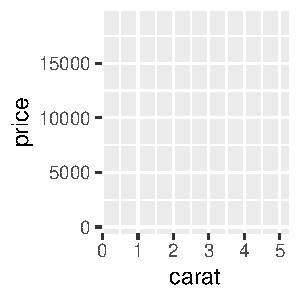
\includegraphics[width=0.5\linewidth]{Figs/unnamed-chunk-2-1} \end{center}
\end{frame}

\begin{frame}[fragile]{Statistics}
\phantomsection\label{statistics-6}
Update the plot to add a smooth trend line. Use the default method,
which uses the LOESS model to fit the curve.

\AddToHookNext{env/Highlighting/begin}{\tiny}

\begin{Shaded}
\begin{Highlighting}[]
\CommentTok{\# Amend the plot to add a smooth layer}
\FunctionTok{ggplot}\NormalTok{(mtcars, }\FunctionTok{aes}\NormalTok{(}\AttributeTok{x =}\NormalTok{ wt, }\AttributeTok{y =}\NormalTok{ mpg)) }\SpecialCharTok{+} \FunctionTok{geom\_point}\NormalTok{() }\SpecialCharTok{+} \FunctionTok{geom\_smooth}\NormalTok{()}
\end{Highlighting}
\end{Shaded}

\begin{center}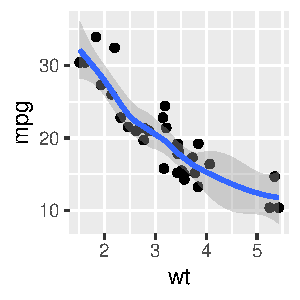
\includegraphics[width=0.5\linewidth]{Figs/unnamed-chunk-3-1} \end{center}
\end{frame}

\begin{frame}[fragile]{Statistics}
\phantomsection\label{statistics-7}
Update the smooth layer.

\AddToHookNext{env/Highlighting/begin}{\tiny}

\begin{Shaded}
\begin{Highlighting}[]
\CommentTok{\# Amend the plot. Use lin. reg. smoothing; turn off std err}
\CommentTok{\# ribbon}
\FunctionTok{ggplot}\NormalTok{(mtcars, }\FunctionTok{aes}\NormalTok{(}\AttributeTok{x =}\NormalTok{ wt, }\AttributeTok{y =}\NormalTok{ mpg)) }\SpecialCharTok{+} \FunctionTok{geom\_point}\NormalTok{() }\SpecialCharTok{+} \FunctionTok{geom\_smooth}\NormalTok{(}\AttributeTok{method =} \StringTok{"lm"}\NormalTok{,}
    \AttributeTok{se =} \ConstantTok{FALSE}\NormalTok{)}
\end{Highlighting}
\end{Shaded}

\begin{center}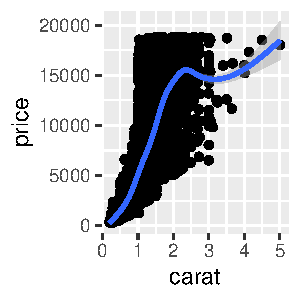
\includegraphics[width=0.5\linewidth]{Figs/unnamed-chunk-4-1} \end{center}

Apply a linear model by setting method to ``lm'', and turn off the
model's \(95\%\) confidence interval (the ribbon) by setting se to
FALSE.
\end{frame}

\begin{frame}[fragile]{Statistics}
\phantomsection\label{statistics-8}
Draw the same plot again, swapping geom\_smooth() for stat\_smooth().

\AddToHookNext{env/Highlighting/begin}{\tiny}

\begin{Shaded}
\begin{Highlighting}[]
\CommentTok{\# Amend the plot. Swap geom\_smooth() for stat\_smooth().}
\FunctionTok{ggplot}\NormalTok{(mtcars, }\FunctionTok{aes}\NormalTok{(}\AttributeTok{x =}\NormalTok{ wt, }\AttributeTok{y =}\NormalTok{ mpg)) }\SpecialCharTok{+} \FunctionTok{geom\_point}\NormalTok{() }\SpecialCharTok{+} \FunctionTok{stat\_smooth}\NormalTok{(}\AttributeTok{method =} \StringTok{"lm"}\NormalTok{,}
    \AttributeTok{se =} \ConstantTok{FALSE}\NormalTok{)}
\end{Highlighting}
\end{Shaded}

\begin{center}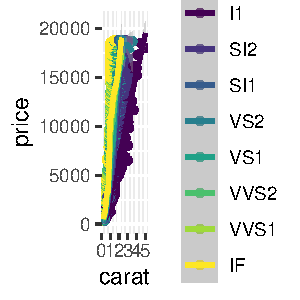
\includegraphics[width=0.5\linewidth]{Figs/unnamed-chunk-5-1} \end{center}
\end{frame}

\begin{frame}{Grouping variables}
\phantomsection\label{grouping-variables}
\begin{itemize}
\item
  We'll continue with the previous exercise by considering the situation
  of looking at sub-groups in our dataset.
\item
  For this we'll encounter the invisible group aesthetic.
\end{itemize}
\end{frame}

\begin{frame}[fragile]{Grouping variables}
\phantomsection\label{grouping-variables-1}
mtcars has been given an extra column, fcyl, that is the cyl column
converted to a proper factor variable.

\AddToHookNext{env/Highlighting/begin}{\tiny}

\begin{Shaded}
\begin{Highlighting}[]
\NormalTok{mtcars }\OtherTok{\textless{}{-}}\NormalTok{ mtcars }\SpecialCharTok{\%\textgreater{}\%}
    \FunctionTok{mutate}\NormalTok{(}\AttributeTok{fcyl =} \FunctionTok{as.factor}\NormalTok{(cyl), }\AttributeTok{fam =} \FunctionTok{as.factor}\NormalTok{(am))}
\end{Highlighting}
\end{Shaded}
\end{frame}

\begin{frame}[fragile]{Grouping variables}
\phantomsection\label{grouping-variables-2}
Using mtcars, plot mpg vs.~wt, colored by fcyl, add a point layer.

\AddToHookNext{env/Highlighting/begin}{\tiny}

\begin{Shaded}
\begin{Highlighting}[]
\FunctionTok{ggplot}\NormalTok{(mtcars, }\FunctionTok{aes}\NormalTok{(}\AttributeTok{x =}\NormalTok{ wt, }\AttributeTok{y =}\NormalTok{ mpg, }\AttributeTok{color =}\NormalTok{ fcyl)) }\SpecialCharTok{+} \FunctionTok{geom\_point}\NormalTok{()}
\end{Highlighting}
\end{Shaded}

\begin{center}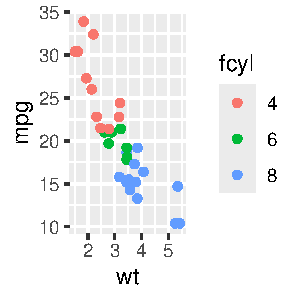
\includegraphics[width=0.5\linewidth]{Figs/unnamed-chunk-7-1} \end{center}
\end{frame}

\begin{frame}[fragile]{Grouping variables}
\phantomsection\label{grouping-variables-3}
Add a smooth stat using a linear model, and don't show the se ribbon.

\AddToHookNext{env/Highlighting/begin}{\tiny}

\begin{Shaded}
\begin{Highlighting}[]
\CommentTok{\# Using mtcars, plot mpg vs. wt, colored by fcyl}
\FunctionTok{ggplot}\NormalTok{(mtcars, }\FunctionTok{aes}\NormalTok{(}\AttributeTok{x =}\NormalTok{ wt, }\AttributeTok{y =}\NormalTok{ mpg, }\AttributeTok{color =}\NormalTok{ fcyl)) }\SpecialCharTok{+} \FunctionTok{geom\_point}\NormalTok{() }\SpecialCharTok{+}
    \FunctionTok{stat\_smooth}\NormalTok{(}\AttributeTok{method =} \StringTok{"lm"}\NormalTok{, }\AttributeTok{se =} \ConstantTok{FALSE}\NormalTok{)}
\end{Highlighting}
\end{Shaded}

\begin{center}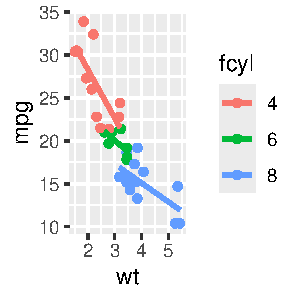
\includegraphics[width=0.5\linewidth]{Figs/unnamed-chunk-8-1} \end{center}
\end{frame}

\begin{frame}[fragile]{Grouping variables}
\phantomsection\label{grouping-variables-4}
Update the plot to add a second smooth stat.

\AddToHookNext{env/Highlighting/begin}{\tiny}

\begin{Shaded}
\begin{Highlighting}[]
\CommentTok{\# Amend the plot to add another smooth layer with dummy}
\CommentTok{\# grouping}
\FunctionTok{ggplot}\NormalTok{(mtcars, }\FunctionTok{aes}\NormalTok{(}\AttributeTok{x =}\NormalTok{ wt, }\AttributeTok{y =}\NormalTok{ mpg, }\AttributeTok{color =}\NormalTok{ fcyl)) }\SpecialCharTok{+} \FunctionTok{geom\_point}\NormalTok{() }\SpecialCharTok{+}
    \FunctionTok{stat\_smooth}\NormalTok{(}\AttributeTok{method =} \StringTok{"lm"}\NormalTok{, }\AttributeTok{se =} \ConstantTok{FALSE}\NormalTok{) }\SpecialCharTok{+} \FunctionTok{stat\_smooth}\NormalTok{(}\FunctionTok{aes}\NormalTok{(}\AttributeTok{group =} \DecValTok{1}\NormalTok{),}
    \AttributeTok{method =} \StringTok{"lm"}\NormalTok{, }\AttributeTok{se =} \ConstantTok{FALSE}\NormalTok{)}
\end{Highlighting}
\end{Shaded}

\begin{center}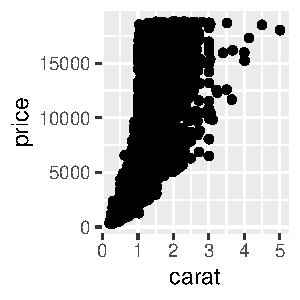
\includegraphics[width=0.5\linewidth]{Figs/unnamed-chunk-9-1} \end{center}

Add a dummy group aesthetic to this layer, setting the value to 1. Use
the same method and se values as the first stat smooth layer.
\end{frame}

\begin{frame}{Grouping variables}
\phantomsection\label{grouping-variables-5}
\begin{itemize}
\item
  In the previous exercise we used se = FALSE in \(stat\_smooth()\) to
  remove the 95\% Confidence Interval.
\item
  Here we'll consider another argument, \textbf{span}, used in LOESS
  smoothing, and we'll take a look at a nice scenario of properly
  mapping different models.
\end{itemize}
\end{frame}

\begin{frame}{Grouping variables}
\phantomsection\label{grouping-variables-6}
\begin{itemize}
\item
  Explore the effect of the span argument on LOESS curves.
\item
  Add three smooth LOESS stats, each without the standard error ribbon.
\end{itemize}
\end{frame}

\begin{frame}{Grouping variables}
\phantomsection\label{grouping-variables-7}
\begin{itemize}
\item
  Color the 1st one ``red''; set its span to 0.9.
\item
  Color the 2nd one ``green''; set its span to 0.6.
\item
  Color the 3rd one ``blue''; set its span to 0.3.
\end{itemize}
\end{frame}

\begin{frame}[fragile]{Grouping variables}
\phantomsection\label{grouping-variables-8}
\AddToHookNext{env/Highlighting/begin}{\tiny}

\begin{Shaded}
\begin{Highlighting}[]
\FunctionTok{ggplot}\NormalTok{(mtcars, }\FunctionTok{aes}\NormalTok{(}\AttributeTok{x =}\NormalTok{ wt, }\AttributeTok{y =}\NormalTok{ mpg)) }\SpecialCharTok{+} \FunctionTok{geom\_point}\NormalTok{() }\SpecialCharTok{+} \FunctionTok{stat\_smooth}\NormalTok{(}\AttributeTok{se =} \ConstantTok{FALSE}\NormalTok{,}
    \AttributeTok{color =} \StringTok{"red"}\NormalTok{, }\AttributeTok{span =} \FloatTok{0.9}\NormalTok{) }\SpecialCharTok{+} \FunctionTok{stat\_smooth}\NormalTok{(}\AttributeTok{se =} \ConstantTok{FALSE}\NormalTok{, }\AttributeTok{color =} \StringTok{"green"}\NormalTok{,}
    \AttributeTok{span =} \FloatTok{0.6}\NormalTok{) }\SpecialCharTok{+} \FunctionTok{stat\_smooth}\NormalTok{(}\AttributeTok{se =} \ConstantTok{FALSE}\NormalTok{, }\AttributeTok{color =} \StringTok{"blue"}\NormalTok{, }\AttributeTok{span =} \FloatTok{0.3}\NormalTok{)}
\end{Highlighting}
\end{Shaded}

\begin{center}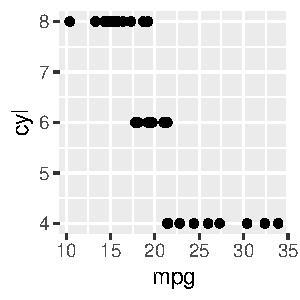
\includegraphics[width=0.5\linewidth]{Figs/unnamed-chunk-10-1} \end{center}
\end{frame}

\begin{frame}[fragile]{Compare LOESS and linear regression smoothing on
small regions of data.}
\phantomsection\label{compare-loess-and-linear-regression-smoothing-on-small-regions-of-data.}
\begin{itemize}
\tightlist
\item
  Add a smooth LOESS stat, without the standard error ribbon.
\end{itemize}

\AddToHookNext{env/Highlighting/begin}{\tiny}

\begin{Shaded}
\begin{Highlighting}[]
\CommentTok{\# Amend the plot to color by fcyl}
\FunctionTok{ggplot}\NormalTok{(mtcars, }\FunctionTok{aes}\NormalTok{(}\AttributeTok{x =}\NormalTok{ wt, }\AttributeTok{y =}\NormalTok{ mpg, }\AttributeTok{color =}\NormalTok{ fcyl)) }\SpecialCharTok{+} \FunctionTok{geom\_point}\NormalTok{() }\SpecialCharTok{+}
    \CommentTok{\# Add a smooth LOESS stat, no ribbon}
\FunctionTok{stat\_smooth}\NormalTok{(}\AttributeTok{se =} \ConstantTok{FALSE}\NormalTok{)}
\end{Highlighting}
\end{Shaded}

\begin{center}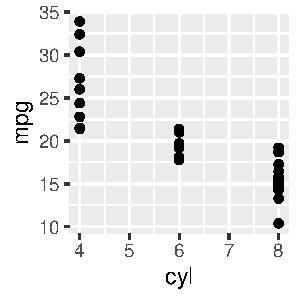
\includegraphics[width=0.5\linewidth]{Figs/unnamed-chunk-11-1} \end{center}
\end{frame}

\begin{frame}[fragile]{Compare LOESS and linear regression smoothing on
small regions of data.}
\phantomsection\label{compare-loess-and-linear-regression-smoothing-on-small-regions-of-data.-1}
Add a smooth linear regression stat, again without the standard error
ribbon.

\AddToHookNext{env/Highlighting/begin}{\tiny}

\begin{Shaded}
\begin{Highlighting}[]
\CommentTok{\# Amend the plot to color by fcyl}
\FunctionTok{ggplot}\NormalTok{(mtcars, }\FunctionTok{aes}\NormalTok{(}\AttributeTok{x =}\NormalTok{ wt, }\AttributeTok{y =}\NormalTok{ mpg, }\AttributeTok{color =}\NormalTok{ fcyl)) }\SpecialCharTok{+} \FunctionTok{geom\_point}\NormalTok{() }\SpecialCharTok{+}
    \FunctionTok{stat\_smooth}\NormalTok{(}\AttributeTok{se =} \ConstantTok{FALSE}\NormalTok{) }\SpecialCharTok{+} \FunctionTok{stat\_smooth}\NormalTok{(}\AttributeTok{method =} \StringTok{"lm"}\NormalTok{, }\AttributeTok{se =} \ConstantTok{FALSE}\NormalTok{)  }\CommentTok{\# Add a smooth lin. reg. stat, no ribbon}
\end{Highlighting}
\end{Shaded}

\begin{center}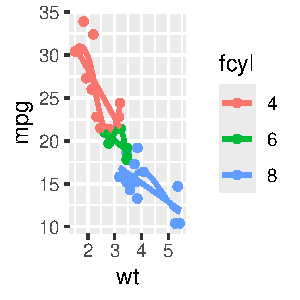
\includegraphics[width=0.5\linewidth]{Figs/unnamed-chunk-12-1} \end{center}

LOESS isn't great on very short sections of data; compare the pieces of
linear regression to LOESS over the whole thing.
\end{frame}

\begin{frame}[fragile]{Compare LOESS and linear regression smoothing on
small regions of data.}
\phantomsection\label{compare-loess-and-linear-regression-smoothing-on-small-regions-of-data.-2}
\begin{itemize}
\tightlist
\item
  Amend the smooth LOESS stat to map color to a dummy variable, ``All''.
\end{itemize}

\AddToHookNext{env/Highlighting/begin}{\tiny}

\begin{Shaded}
\begin{Highlighting}[]
\CommentTok{\# Amend the plot}
\FunctionTok{ggplot}\NormalTok{(mtcars, }\FunctionTok{aes}\NormalTok{(}\AttributeTok{x =}\NormalTok{ wt, }\AttributeTok{y =}\NormalTok{ mpg, }\AttributeTok{color =}\NormalTok{ fcyl)) }\SpecialCharTok{+} \FunctionTok{geom\_point}\NormalTok{() }\SpecialCharTok{+}
    \FunctionTok{stat\_smooth}\NormalTok{(}\FunctionTok{aes}\NormalTok{(}\AttributeTok{color =} \StringTok{"All"}\NormalTok{), }\AttributeTok{se =} \ConstantTok{FALSE}\NormalTok{) }\SpecialCharTok{+} \FunctionTok{stat\_smooth}\NormalTok{(}\AttributeTok{method =} \StringTok{"lm"}\NormalTok{,}
    \AttributeTok{se =} \ConstantTok{FALSE}\NormalTok{)}
\end{Highlighting}
\end{Shaded}

\begin{center}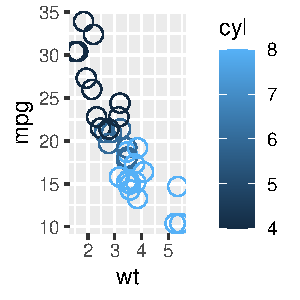
\includegraphics[width=0.5\linewidth]{Figs/unnamed-chunk-13-1} \end{center}
\end{frame}

\begin{frame}{Modifying stat\_smooth (2)}
\phantomsection\label{modifying-stat_smooth-2}
\begin{itemize}
\item
  In this exercise we'll take a look at the standard error ribbons,
  which show the \(95\%\) confidence interval of smoothing models.
\item
  ggplot2 and the Vocab data frame are already loaded for you.
\end{itemize}
\end{frame}

\begin{frame}[fragile]{Modifying stat\_smooth (2)}
\phantomsection\label{modifying-stat_smooth-2-1}
\begin{itemize}
\tightlist
\item
  Vocab has been given an extra column, \(year\_group\), splitting the
  dates into before and after 1995.
\end{itemize}

\AddToHookNext{env/Highlighting/begin}{\tiny}

\begin{Shaded}
\begin{Highlighting}[]
\FunctionTok{library}\NormalTok{(carData)}
\NormalTok{Vocab }\OtherTok{\textless{}{-}}\NormalTok{ Vocab }\SpecialCharTok{\%\textgreater{}\%}
    \FunctionTok{mutate}\NormalTok{(}\AttributeTok{year\_group =} \FunctionTok{as.factor}\NormalTok{(}\FunctionTok{ifelse}\NormalTok{(year }\SpecialCharTok{\textless{}} \DecValTok{1995}\NormalTok{, }\StringTok{"[1974,1995]"}\NormalTok{,}
        \StringTok{"[1995,2016]"}\NormalTok{)))}
\end{Highlighting}
\end{Shaded}
\end{frame}

\begin{frame}[fragile]{Modifying stat\_smooth (2)}
\phantomsection\label{modifying-stat_smooth-2-2}
Using Vocab, plot vocabulary vs.~education, colored by year\_group. Use
geom\_jitter() to add jittered points with transparency 0.25.

\AddToHookNext{env/Highlighting/begin}{\tiny}

\begin{Shaded}
\begin{Highlighting}[]
\CommentTok{\# Plot vocabulary vs. education, colored by year\_group}
\FunctionTok{ggplot}\NormalTok{(Vocab, }\FunctionTok{aes}\NormalTok{(}\AttributeTok{x =}\NormalTok{ education, }\AttributeTok{y =}\NormalTok{ vocabulary, }\AttributeTok{color =}\NormalTok{ year\_group)) }\SpecialCharTok{+}
    \FunctionTok{geom\_jitter}\NormalTok{(}\AttributeTok{alpha =} \FloatTok{0.25}\NormalTok{)}
\end{Highlighting}
\end{Shaded}

\begin{center}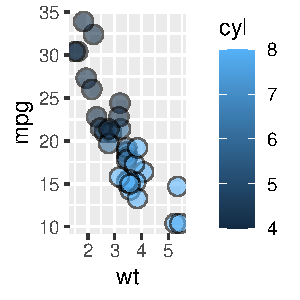
\includegraphics[width=0.5\linewidth]{Figs/unnamed-chunk-15-1} \end{center}
\end{frame}

\begin{frame}[fragile]{Modifying stat\_smooth (2)}
\phantomsection\label{modifying-stat_smooth-2-3}
Add a smooth linear regression stat (with the standard error ribbon).

\AddToHookNext{env/Highlighting/begin}{\tiny}

\begin{Shaded}
\begin{Highlighting}[]
\CommentTok{\# Plot vocabulary vs. education, colored by year\_group}
\FunctionTok{ggplot}\NormalTok{(Vocab, }\FunctionTok{aes}\NormalTok{(}\AttributeTok{x =}\NormalTok{ education, }\AttributeTok{y =}\NormalTok{ vocabulary, }\AttributeTok{color =}\NormalTok{ year\_group)) }\SpecialCharTok{+}
    \FunctionTok{geom\_jitter}\NormalTok{(}\AttributeTok{alpha =} \FloatTok{0.25}\NormalTok{) }\SpecialCharTok{+} \FunctionTok{stat\_smooth}\NormalTok{(}\AttributeTok{method =} \StringTok{"lm"}\NormalTok{)}
\end{Highlighting}
\end{Shaded}

\begin{center}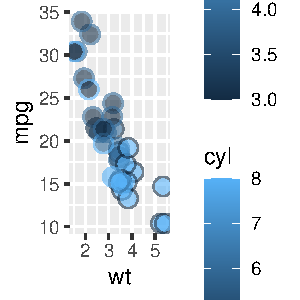
\includegraphics[width=0.5\linewidth]{Figs/unnamed-chunk-16-1} \end{center}
\end{frame}

\begin{frame}[fragile]{Modifying stat\_smooth (2)}
\phantomsection\label{modifying-stat_smooth-2-4}
It's easier to read the plot if the standard error ribbons match the
lines, and the lines have more emphasis.

Update the smooth stat. Map the fill color to \(year\_group\).

\AddToHookNext{env/Highlighting/begin}{\tiny}

\begin{Shaded}
\begin{Highlighting}[]
\CommentTok{\# Amend the plot}
\FunctionTok{ggplot}\NormalTok{(Vocab, }\FunctionTok{aes}\NormalTok{(}\AttributeTok{x =}\NormalTok{ education, }\AttributeTok{y =}\NormalTok{ vocabulary, }\AttributeTok{color =}\NormalTok{ year\_group)) }\SpecialCharTok{+}
    \FunctionTok{geom\_jitter}\NormalTok{(}\AttributeTok{alpha =} \FloatTok{0.25}\NormalTok{) }\SpecialCharTok{+} \FunctionTok{stat\_smooth}\NormalTok{(}\FunctionTok{aes}\NormalTok{(}\AttributeTok{fill =}\NormalTok{ year\_group),}
    \AttributeTok{method =} \StringTok{"lm"}\NormalTok{, }\AttributeTok{size =} \DecValTok{2}\NormalTok{)  }\CommentTok{\# Map the fill color to year\_group, set the line size to 2}
\end{Highlighting}
\end{Shaded}

\begin{center}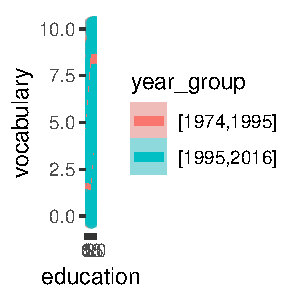
\includegraphics[width=0.5\linewidth]{Figs/unnamed-chunk-17-1} \end{center}

Set the line size to 2.
\end{frame}

\begin{frame}{Quantiles}
\phantomsection\label{quantiles}
Here, we'll continue with the \textbf{Vocab} dataset and use
\(stat\_quantile()\) to apply a quantile regression.
\end{frame}

\begin{frame}{Quantiles}
\phantomsection\label{quantiles-1}
Linear regression predicts the mean response from the explanatory
variables, quantile regression predicts a quantile response (e.g.~the
median) from the explanatory variables. Specific quantiles can be
specified with the quantiles argument.
\end{frame}

\begin{frame}{Quantiles}
\phantomsection\label{quantiles-2}
\begin{itemize}
\item
  Specifying many quantiles and color your models according to year can
  make plots too busy.
\item
  We'll explore ways of dealing with this in the next chapter.
\end{itemize}
\end{frame}

\begin{frame}[fragile]{Quantiles}
\phantomsection\label{quantiles-3}
Update the plot to add a quantile regression stat, at quantiles 0.05,
0.5, and 0.95.

\AddToHookNext{env/Highlighting/begin}{\tiny}

\begin{Shaded}
\begin{Highlighting}[]
\FunctionTok{ggplot}\NormalTok{(Vocab, }\FunctionTok{aes}\NormalTok{(}\AttributeTok{x =}\NormalTok{ education, }\AttributeTok{y =}\NormalTok{ vocabulary)) }\SpecialCharTok{+} \FunctionTok{geom\_jitter}\NormalTok{(}\AttributeTok{alpha =} \FloatTok{0.25}\NormalTok{) }\SpecialCharTok{+}
    \FunctionTok{stat\_quantile}\NormalTok{(}\AttributeTok{quantiles =} \FunctionTok{c}\NormalTok{(}\FloatTok{0.05}\NormalTok{, }\FloatTok{0.5}\NormalTok{, }\FloatTok{0.95}\NormalTok{))  }\CommentTok{\# Add a quantile stat, at 0.05, 0.5, and 0.95}
\end{Highlighting}
\end{Shaded}

\begin{center}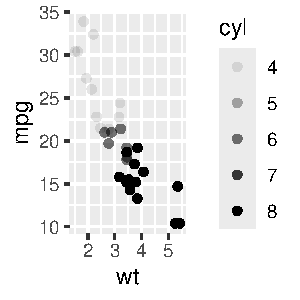
\includegraphics[width=0.5\linewidth]{Figs/unnamed-chunk-18-1} \end{center}
\end{frame}

\begin{frame}[fragile]{Quantiles}
\phantomsection\label{quantiles-4}
Amend the plot to color according to \(year\_group\).

\AddToHookNext{env/Highlighting/begin}{\tiny}

\begin{Shaded}
\begin{Highlighting}[]
\CommentTok{\# Amend the plot to color by year\_group}
\FunctionTok{ggplot}\NormalTok{(Vocab, }\FunctionTok{aes}\NormalTok{(}\AttributeTok{x =}\NormalTok{ education, }\AttributeTok{y =}\NormalTok{ vocabulary, }\AttributeTok{color =}\NormalTok{ year\_group)) }\SpecialCharTok{+}
    \FunctionTok{geom\_jitter}\NormalTok{(}\AttributeTok{alpha =} \FloatTok{0.25}\NormalTok{) }\SpecialCharTok{+} \FunctionTok{stat\_quantile}\NormalTok{(}\AttributeTok{quantiles =} \FunctionTok{c}\NormalTok{(}\FloatTok{0.05}\NormalTok{,}
    \FloatTok{0.5}\NormalTok{, }\FloatTok{0.95}\NormalTok{))}
\end{Highlighting}
\end{Shaded}

\begin{center}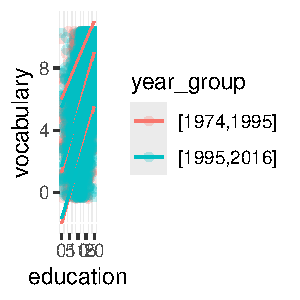
\includegraphics[width=0.5\linewidth]{Figs/unnamed-chunk-19-1} \end{center}
\end{frame}

\begin{frame}{Using \(stat\_sum()\)}
\phantomsection\label{using-stat_sum}
\begin{itemize}
\item
  In the first course, you saw that this is one of the four causes of
  overplotting.
\item
  You'd get a single point at each intersection between the two
  variables.
\end{itemize}
\end{frame}

\begin{frame}{Using \(stat\_sum()\)}
\phantomsection\label{using-stat_sum-1}
\begin{itemize}
\item
  One solution, shown in the step 1, is jittering with transparency.
\item
  Another solution is to use \(stat\_sum()\), which calculates the total
  number of overlapping observations and maps that onto the size
  aesthetic.
\end{itemize}
\end{frame}

\begin{frame}{Using \(stat\_sum()\)}
\phantomsection\label{using-stat_sum-2}
Using \(stat\_sum()\) allows a special variable, prop.., to show the
proportion of values within the dataset.
\end{frame}

\begin{frame}[fragile]{Using \(stat\_sum()\)}
\phantomsection\label{using-stat_sum-3}
Run the code to see how jittering \& transparency solves overplotting.

\AddToHookNext{env/Highlighting/begin}{\tiny}

\begin{Shaded}
\begin{Highlighting}[]
\CommentTok{\# Plot vocabulary vs. education, colored by year\_group}
\FunctionTok{ggplot}\NormalTok{(Vocab, }\FunctionTok{aes}\NormalTok{(}\AttributeTok{x =}\NormalTok{ education, }\AttributeTok{y =}\NormalTok{ vocabulary, }\AttributeTok{color =}\NormalTok{ year\_group)) }\SpecialCharTok{+}
    \FunctionTok{geom\_jitter}\NormalTok{(}\AttributeTok{alpha =} \FloatTok{0.25}\NormalTok{)  }\CommentTok{\# Add jittered points with transparency 0.25}
\end{Highlighting}
\end{Shaded}

\begin{center}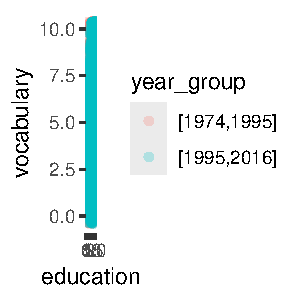
\includegraphics[width=0.5\linewidth]{Figs/unnamed-chunk-20-1} \end{center}
\end{frame}

\begin{frame}[fragile]{Using \(stat\_sum()\)}
\phantomsection\label{using-stat_sum-4}
Replace the jittered points with a sum stat, using stat\_sum().

\AddToHookNext{env/Highlighting/begin}{\tiny}

\begin{Shaded}
\begin{Highlighting}[]
\FunctionTok{ggplot}\NormalTok{(Vocab, }\FunctionTok{aes}\NormalTok{(}\AttributeTok{x =}\NormalTok{ education, }\AttributeTok{y =}\NormalTok{ vocabulary)) }\SpecialCharTok{+} \FunctionTok{stat\_sum}\NormalTok{()}
\end{Highlighting}
\end{Shaded}

\begin{center}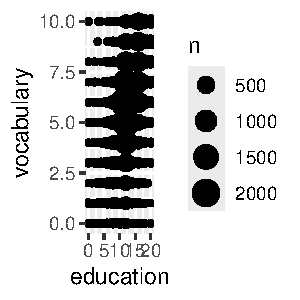
\includegraphics[width=0.5\linewidth]{Figs/unnamed-chunk-21-1} \end{center}
\end{frame}

\begin{frame}[fragile]{Using \(stat\_sum()\)}
\phantomsection\label{using-stat_sum-5}
Modify the size aesthetic with the appropriate scale function.

\AddToHookNext{env/Highlighting/begin}{\tiny}

\begin{Shaded}
\begin{Highlighting}[]
\FunctionTok{ggplot}\NormalTok{(Vocab, }\FunctionTok{aes}\NormalTok{(}\AttributeTok{x =}\NormalTok{ education, }\AttributeTok{y =}\NormalTok{ vocabulary)) }\SpecialCharTok{+} \FunctionTok{stat\_sum}\NormalTok{() }\SpecialCharTok{+}
    \CommentTok{\# Add a size scale, from 1 to 10}
\FunctionTok{scale\_size}\NormalTok{(}\AttributeTok{range =} \FunctionTok{c}\NormalTok{(}\DecValTok{1}\NormalTok{, }\DecValTok{10}\NormalTok{))}
\end{Highlighting}
\end{Shaded}

\begin{center}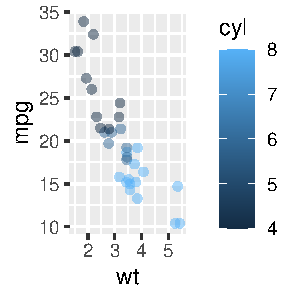
\includegraphics[width=0.5\linewidth]{Figs/unnamed-chunk-22-1} \end{center}

Add a \(scale\_size()\) function to set the range from 1 to 10.
\end{frame}

\begin{frame}[fragile]{Using \(stat\_sum()\)}
\phantomsection\label{using-stat_sum-6}
Inside \(stat\_sum()\) , set \textbf{size} to ..prop.. so circle size
represents the proportion of the whole dataset.

\AddToHookNext{env/Highlighting/begin}{\tiny}

\begin{Shaded}
\begin{Highlighting}[]
\CommentTok{\# Amend the stat to use proportion sizes}
\FunctionTok{ggplot}\NormalTok{(Vocab, }\FunctionTok{aes}\NormalTok{(}\AttributeTok{x =}\NormalTok{ education, }\AttributeTok{y =}\NormalTok{ vocabulary)) }\SpecialCharTok{+} \FunctionTok{stat\_sum}\NormalTok{(}\FunctionTok{aes}\NormalTok{(}\AttributeTok{size =}\NormalTok{ ..prop..))}
\end{Highlighting}
\end{Shaded}

\begin{center}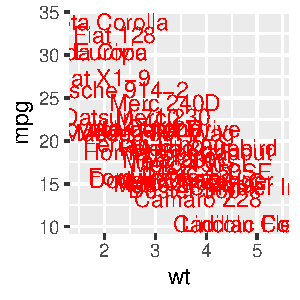
\includegraphics[width=0.5\linewidth]{Figs/unnamed-chunk-23-1} \end{center}
\end{frame}

\begin{frame}[fragile]{Using \(stat\_sum()\)}
\phantomsection\label{using-stat_sum-7}
Update the plot to group by education, so that circle size represents
the proportion of the group.

\AddToHookNext{env/Highlighting/begin}{\tiny}

\begin{Shaded}
\begin{Highlighting}[]
\CommentTok{\# Amend the plot to group by education}
\FunctionTok{ggplot}\NormalTok{(Vocab, }\FunctionTok{aes}\NormalTok{(}\AttributeTok{x =}\NormalTok{ education, }\AttributeTok{y =}\NormalTok{ vocabulary, }\AttributeTok{group =}\NormalTok{ education)) }\SpecialCharTok{+}
    \FunctionTok{stat\_sum}\NormalTok{(}\FunctionTok{aes}\NormalTok{(}\AttributeTok{size =}\NormalTok{ ..prop..))}
\end{Highlighting}
\end{Shaded}

\begin{center}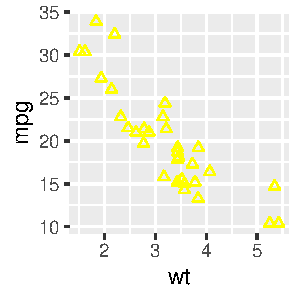
\includegraphics[width=0.5\linewidth]{Figs/unnamed-chunk-24-1} \end{center}
\end{frame}

\begin{frame}{Stats outside geoms}
\phantomsection\label{stats-outside-geoms}
\begin{itemize}
\item
  Preparations In the following exercises, we'll aim to make the plot
  shown in the viewer.
\item
  Here, we'll establish our positions and base layer of the plot.
\item
  Establishing these items as independent objects will allow us to
  recycle them easily in many layers, or plots.
\end{itemize}
\end{frame}

\begin{frame}{Stats outside geoms}
\phantomsection\label{stats-outside-geoms-1}
\(position\_jitter()\) adds jittering (e.g.~for points).

\(position\_dodge()\) dodges geoms, (e.g.~bar, col, boxplot, violin,
errorbar, pointrange).

\(position\_jitterdodge()\) jitters and dodges geoms, (e.g.~points).
\end{frame}

\begin{frame}{Stats outside geoms}
\phantomsection\label{stats-outside-geoms-2}
As before, we'll use \textbf{mtcars}, where \textbf{fcyl} and
\textbf{fam} are proper factor variables of the original cyl and am
variables.
\end{frame}

\begin{frame}[fragile]{Stats outside geoms}
\phantomsection\label{stats-outside-geoms-3}
Using these three functions, define these position objects:

\begin{itemize}
\tightlist
\item
  \(posn\_j:\) will jitter with a width of 0.2.
\end{itemize}

\AddToHookNext{env/Highlighting/begin}{\tiny}

\begin{Shaded}
\begin{Highlighting}[]
\CommentTok{\# Define position objects 1. Jitter with width 0.2}
\NormalTok{posn\_j }\OtherTok{\textless{}{-}} \FunctionTok{position\_jitter}\NormalTok{(}\AttributeTok{width =} \FloatTok{0.2}\NormalTok{)}

\CommentTok{\# 2. Dodge with width 0.1}
\NormalTok{posn\_d }\OtherTok{\textless{}{-}} \FunctionTok{position\_dodge}\NormalTok{(}\AttributeTok{width =} \FloatTok{0.1}\NormalTok{)}

\CommentTok{\# 3. Jitter{-}dodge with jitter.width 0.2 and dodge.width 0.1}
\NormalTok{posn\_jd }\OtherTok{\textless{}{-}} \FunctionTok{position\_jitterdodge}\NormalTok{(}\AttributeTok{jitter.width =} \FloatTok{0.2}\NormalTok{, }\AttributeTok{dodge.width =} \FloatTok{0.1}\NormalTok{)}
\end{Highlighting}
\end{Shaded}
\end{frame}

\begin{frame}[fragile]{Stats outside geoms}
\phantomsection\label{stats-outside-geoms-4}
Using these three functions, define these position objects:

\begin{itemize}
\tightlist
\item
  \(posn\_d:\) will dodge with a width of 0.1.
\end{itemize}

\AddToHookNext{env/Highlighting/begin}{\tiny}

\begin{Shaded}
\begin{Highlighting}[]
\CommentTok{\# Define position objects 1. Jitter with width 0.2}
\NormalTok{posn\_j }\OtherTok{\textless{}{-}} \FunctionTok{position\_jitter}\NormalTok{(}\AttributeTok{width =} \FloatTok{0.2}\NormalTok{)}

\CommentTok{\# 2. Dodge with width 0.1}
\NormalTok{posn\_d }\OtherTok{\textless{}{-}} \FunctionTok{position\_dodge}\NormalTok{(}\AttributeTok{width =} \FloatTok{0.1}\NormalTok{)}

\CommentTok{\# 3. Jitter{-}dodge with jitter.width 0.2 and dodge.width 0.1}
\NormalTok{posn\_jd }\OtherTok{\textless{}{-}} \FunctionTok{position\_jitterdodge}\NormalTok{(}\AttributeTok{jitter.width =} \FloatTok{0.2}\NormalTok{, }\AttributeTok{dodge.width =} \FloatTok{0.1}\NormalTok{)}
\end{Highlighting}
\end{Shaded}
\end{frame}

\begin{frame}[fragile]{Stats outside geoms}
\phantomsection\label{stats-outside-geoms-5}
Using these three functions, define these position objects:

\begin{itemize}
\tightlist
\item
  \(posn\_jd\) will jitter and dodge with a jitter.width of 0.2 and a
  dodge.width of 0.1.
\end{itemize}

\AddToHookNext{env/Highlighting/begin}{\tiny}

\begin{Shaded}
\begin{Highlighting}[]
\CommentTok{\# Define position objects 1. Jitter with width 0.2}
\NormalTok{posn\_j }\OtherTok{\textless{}{-}} \FunctionTok{position\_jitter}\NormalTok{(}\AttributeTok{width =} \FloatTok{0.2}\NormalTok{)}

\CommentTok{\# 2. Dodge with width 0.1}
\NormalTok{posn\_d }\OtherTok{\textless{}{-}} \FunctionTok{position\_dodge}\NormalTok{(}\AttributeTok{width =} \FloatTok{0.1}\NormalTok{)}

\CommentTok{\# 3. Jitter{-}dodge with jitter.width 0.2 and dodge.width 0.1}
\NormalTok{posn\_jd }\OtherTok{\textless{}{-}} \FunctionTok{position\_jitterdodge}\NormalTok{(}\AttributeTok{jitter.width =} \FloatTok{0.2}\NormalTok{, }\AttributeTok{dodge.width =} \FloatTok{0.1}\NormalTok{)}
\end{Highlighting}
\end{Shaded}
\end{frame}

\begin{frame}[fragile]{Stats outside geoms}
\phantomsection\label{stats-outside-geoms-6}
Plot wt vs.~fcyl, colored by fam.

\AddToHookNext{env/Highlighting/begin}{\tiny}

\begin{Shaded}
\begin{Highlighting}[]
\CommentTok{\# Create the plot base: wt vs. fcyl, colored by fam}
\NormalTok{p\_wt\_vs\_fcyl\_by\_fam }\OtherTok{\textless{}{-}} \FunctionTok{ggplot}\NormalTok{(mtcars, }\FunctionTok{aes}\NormalTok{(}\AttributeTok{x =}\NormalTok{ fcyl, }\AttributeTok{y =}\NormalTok{ wt, }\AttributeTok{color =}\NormalTok{ fam))}
\end{Highlighting}
\end{Shaded}

Assign this base layer to \(p\_wt\_vs\_fcyl\_by\_fam\).
\end{frame}

\begin{frame}[fragile]{Stats outside geoms}
\phantomsection\label{stats-outside-geoms-7}
Plot the data using \(geom\_point()\).

\AddToHookNext{env/Highlighting/begin}{\tiny}

\begin{Shaded}
\begin{Highlighting}[]
\CommentTok{\# Add a point layer}
\NormalTok{p\_wt\_vs\_fcyl\_by\_fam }\SpecialCharTok{+} \FunctionTok{geom\_point}\NormalTok{()}
\end{Highlighting}
\end{Shaded}

\begin{center}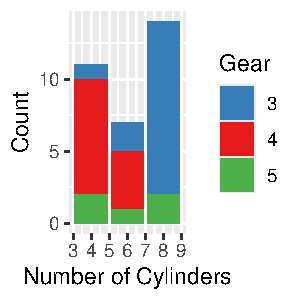
\includegraphics[width=0.5\linewidth]{Figs/unnamed-chunk-29-1} \end{center}
\end{frame}

\begin{frame}{Using position objects}
\phantomsection\label{using-position-objects}
\begin{itemize}
\item
  Now that the position objects have been created, you can apply them to
  the base plot to see their effects.
\item
  You do this by adding a point geom and setting the position argument
  to the position object.
\end{itemize}
\end{frame}

\begin{frame}[fragile]{Using position objects}
\phantomsection\label{using-position-objects-1}
Apply the jitter position, \(posn\_j\), to the base plot.

\AddToHookNext{env/Highlighting/begin}{\tiny}

\begin{Shaded}
\begin{Highlighting}[]
\CommentTok{\# Add jittering only}
\NormalTok{p\_wt\_vs\_fcyl\_by\_fam }\SpecialCharTok{+} \FunctionTok{geom\_point}\NormalTok{(}\AttributeTok{position =}\NormalTok{ posn\_j)}
\end{Highlighting}
\end{Shaded}

\begin{center}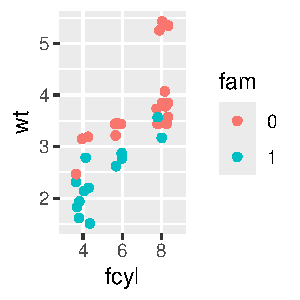
\includegraphics[width=0.5\linewidth]{Figs/unnamed-chunk-30-1} \end{center}
\end{frame}

\begin{frame}[fragile]{Using position objects}
\phantomsection\label{using-position-objects-2}
Apply the dodge position, \(posn\_d\), to the base plot.

\AddToHookNext{env/Highlighting/begin}{\tiny}

\begin{Shaded}
\begin{Highlighting}[]
\CommentTok{\# Add dodging only}
\NormalTok{p\_wt\_vs\_fcyl\_by\_fam }\SpecialCharTok{+} \FunctionTok{geom\_point}\NormalTok{(}\AttributeTok{position =}\NormalTok{ posn\_d)}
\end{Highlighting}
\end{Shaded}

\begin{center}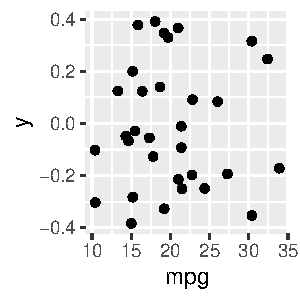
\includegraphics[width=0.5\linewidth]{Figs/unnamed-chunk-31-1} \end{center}

Plotting variations The preparation is done; now let's explore
\(stat\_summary()\).
\end{frame}

\begin{frame}{\(stat\_summary()\)}
\phantomsection\label{stat_summary}
Summary statistics refers to a combination of location (mean or median)
and spread (standard deviation or confidence interval).

These metrics are calculated in \(stat\_summary()\) by passing a
function to the fun.data argument.
\end{frame}

\begin{frame}{\(stat\_summary()\)}
\phantomsection\label{stat_summary-1}
\(mean\_sdl()\), calculates multiples of the standard deviation and
\(mean\_cl\_normal()\) calculates the t-corrected 95\% CI.

Arguments to the data function are passed to stat\_summary()'s fun.args
argument as a list.
\end{frame}

\begin{frame}[fragile]{\(stat\_summary()\)}
\phantomsection\label{stat_summary-2}
Let's start with basic plot

\AddToHookNext{env/Highlighting/begin}{\tiny}

\begin{Shaded}
\begin{Highlighting}[]
\CommentTok{\# Example dataset}
\FunctionTok{data}\NormalTok{(mtcars)}
\CommentTok{\# Define position dodge}
\NormalTok{posn\_d }\OtherTok{\textless{}{-}} \FunctionTok{position\_dodge}\NormalTok{(}\AttributeTok{width =} \FloatTok{0.2}\NormalTok{)}
\CommentTok{\# Base plot}
\NormalTok{p\_wt\_vs\_fcyl\_by\_fam }\OtherTok{\textless{}{-}} \FunctionTok{ggplot}\NormalTok{(mtcars, }\FunctionTok{aes}\NormalTok{(}\AttributeTok{x =} \FunctionTok{factor}\NormalTok{(cyl), }\AttributeTok{y =}\NormalTok{ wt,}
    \AttributeTok{color =} \FunctionTok{factor}\NormalTok{(am))) }\SpecialCharTok{+} \FunctionTok{geom\_point}\NormalTok{(}\AttributeTok{position =}\NormalTok{ posn\_d) }\SpecialCharTok{+} \FunctionTok{labs}\NormalTok{(}\AttributeTok{x =} \StringTok{"Number of Cylinders"}\NormalTok{,}
    \AttributeTok{y =} \StringTok{"Weight"}\NormalTok{, }\AttributeTok{color =} \StringTok{"Transmission (0 = Auto, 1 = Manual)"}\NormalTok{)}
\end{Highlighting}
\end{Shaded}
\end{frame}

\begin{frame}[fragile]{\(stat\_summary()\)}
\phantomsection\label{stat_summary-3}
Add error bars representing the standard deviation.

\AddToHookNext{env/Highlighting/begin}{\tiny}

\begin{Shaded}
\begin{Highlighting}[]
\CommentTok{\# Plot with standard deviation error bars}
\NormalTok{p\_wt\_vs\_fcyl\_by\_fam }\SpecialCharTok{+} \FunctionTok{stat\_summary}\NormalTok{(}\AttributeTok{geom =} \StringTok{"errorbar"}\NormalTok{, }\AttributeTok{position =}\NormalTok{ posn\_d,}
    \AttributeTok{width =} \FloatTok{0.2}\NormalTok{)}
\end{Highlighting}
\end{Shaded}

\begin{center}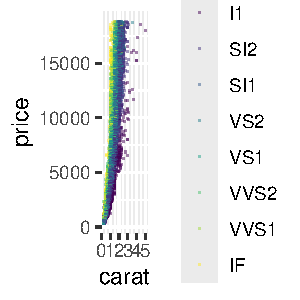
\includegraphics[width=0.5\linewidth]{Figs/unnamed-chunk-33-1} \end{center}
\end{frame}

\begin{frame}[fragile]{\(stat\_summary()\)}
\phantomsection\label{stat_summary-4}
Set the data function to \(mean\_sdl\) (without parentheses).

Draw 1 standard deviation each side of the mean, pass arguments to the
\(mean\_sdl\) function by assigning them to fun.args in the form of a
list.

\AddToHookNext{env/Highlighting/begin}{\tiny}

\begin{Shaded}
\begin{Highlighting}[]
\NormalTok{p\_wt\_vs\_fcyl\_by\_fam }\SpecialCharTok{+} \FunctionTok{stat\_summary}\NormalTok{(}\AttributeTok{fun.data =}\NormalTok{ mean\_sdl, }\AttributeTok{fun.args =} \FunctionTok{list}\NormalTok{(}\AttributeTok{mult =} \DecValTok{1}\NormalTok{),}
    \AttributeTok{position =}\NormalTok{ posn\_d)}
\end{Highlighting}
\end{Shaded}

\begin{center}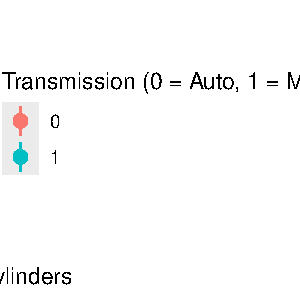
\includegraphics[width=0.5\linewidth]{Figs/unnamed-chunk-34-1} \end{center}

Use \(posn\_d\) to set the position. The default geom for
\(stat\_summary()\) is ``pointrange'' which is already great.
\end{frame}

\begin{frame}[fragile]{\(stat\_summary()\)}
\phantomsection\label{stat_summary-5}
\begin{itemize}
\tightlist
\item
  Update the summary stat to use an ``errorbar'' geom by assigning it to
  the geom argument.
\end{itemize}

\AddToHookNext{env/Highlighting/begin}{\tiny}

\begin{Shaded}
\begin{Highlighting}[]
\NormalTok{p\_wt\_vs\_fcyl\_by\_fam }\SpecialCharTok{+} \FunctionTok{stat\_summary}\NormalTok{(}\AttributeTok{fun.data =}\NormalTok{ mean\_sdl, }\AttributeTok{geom =} \StringTok{"errorbar"}\NormalTok{,}
    \AttributeTok{fun.args =} \FunctionTok{list}\NormalTok{(}\AttributeTok{mult =} \DecValTok{1}\NormalTok{), }\AttributeTok{position =}\NormalTok{ posn\_d)}
\end{Highlighting}
\end{Shaded}

\begin{center}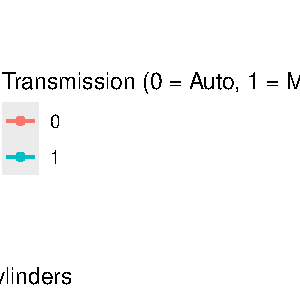
\includegraphics[width=0.5\linewidth]{Figs/unnamed-chunk-35-1} \end{center}

\begin{itemize}
\tightlist
\item
  Update the plot to add a summary stat of 95\% confidence limits.
\end{itemize}
\end{frame}

\begin{frame}[fragile]{\(stat\_summary()\)}
\phantomsection\label{stat_summary-6}
\AddToHookNext{env/Highlighting/begin}{\tiny}

\begin{Shaded}
\begin{Highlighting}[]
\CommentTok{\# Define position dodge}
\NormalTok{posn\_d }\OtherTok{\textless{}{-}} \FunctionTok{position\_dodge}\NormalTok{(}\AttributeTok{width =} \FloatTok{0.2}\NormalTok{)  }
\CommentTok{\# Add summary stat with 95\% confidence limits using mean\_cl\_normal}
\NormalTok{p\_wt\_vs\_fcyl\_by\_fam }\SpecialCharTok{+}
  \FunctionTok{stat\_summary}\NormalTok{(}
    \AttributeTok{fun.data =}\NormalTok{ mean\_cl\_normal,  }\CommentTok{\# Compute 95\% confidence limits}
    \AttributeTok{geom =} \StringTok{"errorbar"}\NormalTok{,          }\CommentTok{\# Use error bars}
    \AttributeTok{position =}\NormalTok{ posn\_d,          }\CommentTok{\# Apply dodge position}
    \AttributeTok{width =} \FloatTok{0.2}                 \CommentTok{\# Set width of error bars}
\NormalTok{  )}
\end{Highlighting}
\end{Shaded}

\begin{center}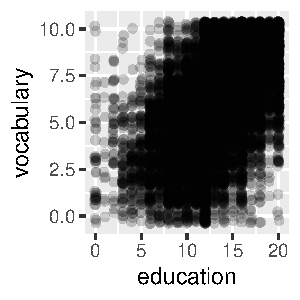
\includegraphics[width=0.5\linewidth]{Figs/unnamed-chunk-36-1} \end{center}

Set the data function to mean\_cl\_normal (without parentheses). Again,
use the dodge position.
\end{frame}

\section{Coordinates}\label{coordinates}

\begin{frame}{Coordinates}
\phantomsection\label{coordinates-1}
The Coordinates layers offer specific and very useful tools for
efficiently and accurately communicating data.
\end{frame}

\begin{frame}{Coordinates}
\phantomsection\label{coordinates-2}
Here we'll look at the various ways of effectively using these layers,
so you can clearly visualize lognormal datasets, variables with units,
and periodic data.
\end{frame}

\begin{frame}{Coordinates}
\phantomsection\label{coordinates-3}
Coordinates Zooming In In the video, you saw different ways of using the
coordinates layer to zoom in.

In this exercise, we'll compare zooming by changing scales and by
changing coordinates.
\end{frame}

\begin{frame}{Coordinates}
\phantomsection\label{coordinates-4}
The big difference is that the scale functions change the underlying
dataset, which affects calculations made by computed geoms (like
histograms or smooth trend lines), whereas coordinate functions make no
changes to the dataset.
\end{frame}

\begin{frame}[fragile]{Coordinates}
\phantomsection\label{coordinates-5}
A scatter plot using mtcars with a LOESS smoothed trend line is
provided. Take a look at this before updating it.

\AddToHookNext{env/Highlighting/begin}{\tiny}

\begin{Shaded}
\begin{Highlighting}[]
\NormalTok{mtcars }\OtherTok{\textless{}{-}}\NormalTok{ mtcars }\SpecialCharTok{\%\textgreater{}\%}
    \FunctionTok{mutate}\NormalTok{(}\AttributeTok{fcyl =} \FunctionTok{as.factor}\NormalTok{(cyl), }\AttributeTok{fam =} \FunctionTok{as.factor}\NormalTok{(am))}
\end{Highlighting}
\end{Shaded}
\end{frame}

\begin{frame}[fragile]{Coordinates}
\phantomsection\label{coordinates-6}
\AddToHookNext{env/Highlighting/begin}{\tiny}

\begin{Shaded}
\begin{Highlighting}[]
\CommentTok{\# Run the code, view the plot, then update it}
\FunctionTok{ggplot}\NormalTok{(mtcars, }\FunctionTok{aes}\NormalTok{(}\AttributeTok{x =}\NormalTok{ wt, }\AttributeTok{y =}\NormalTok{ hp, }\AttributeTok{color =}\NormalTok{ fam)) }\SpecialCharTok{+} \FunctionTok{geom\_point}\NormalTok{() }\SpecialCharTok{+}
    \FunctionTok{geom\_smooth}\NormalTok{()}
\end{Highlighting}
\end{Shaded}

\begin{center}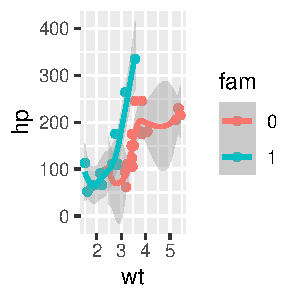
\includegraphics[width=0.5\linewidth]{Figs/unnamed-chunk-38-1} \end{center}
\end{frame}

\begin{frame}[fragile]{Coordinates}
\phantomsection\label{coordinates-7}
Update the plot by adding (+) a continuous x scale with limits from 3 to
6. Spoiler: this will cause a problem!

\AddToHookNext{env/Highlighting/begin}{\tiny}

\begin{Shaded}
\begin{Highlighting}[]
\CommentTok{\# Run the code, view the plot, then update it}
\FunctionTok{ggplot}\NormalTok{(mtcars, }\FunctionTok{aes}\NormalTok{(}\AttributeTok{x =}\NormalTok{ wt, }\AttributeTok{y =}\NormalTok{ hp, }\AttributeTok{color =}\NormalTok{ fam)) }\SpecialCharTok{+} \FunctionTok{geom\_point}\NormalTok{() }\SpecialCharTok{+}
    \FunctionTok{geom\_smooth}\NormalTok{() }\SpecialCharTok{+} \FunctionTok{scale\_x\_continuous}\NormalTok{(}\AttributeTok{limits =} \FunctionTok{c}\NormalTok{(}\DecValTok{3}\NormalTok{, }\DecValTok{6}\NormalTok{))  }\CommentTok{\# Add a continuous x scale with x limits from 3 to 6}
\end{Highlighting}
\end{Shaded}

\begin{center}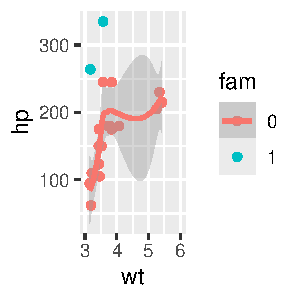
\includegraphics[width=0.5\linewidth]{Figs/unnamed-chunk-39-1} \end{center}
\end{frame}

\begin{frame}[fragile]{Coordinates}
\phantomsection\label{coordinates-8}
Update the plot by adding a Cartesian coordinate system with x limits,
xlim, from 3 to 6.

\AddToHookNext{env/Highlighting/begin}{\tiny}

\begin{Shaded}
\begin{Highlighting}[]
\FunctionTok{ggplot}\NormalTok{(mtcars, }\FunctionTok{aes}\NormalTok{(}\AttributeTok{x =}\NormalTok{ wt, }\AttributeTok{y =}\NormalTok{ hp, }\AttributeTok{color =}\NormalTok{ fam)) }\SpecialCharTok{+} \FunctionTok{geom\_point}\NormalTok{() }\SpecialCharTok{+}
    \FunctionTok{geom\_smooth}\NormalTok{() }\SpecialCharTok{+} \CommentTok{\# Add Cartesian coordinates with x limits from 3 to 6 geom\_smooth()}
    \FunctionTok{geom\_smooth}\NormalTok{() }\SpecialCharTok{+} \CommentTok{\# Add Cartesian coordinates with x limits from 3 to 6 +}
    \FunctionTok{geom\_smooth}\NormalTok{() }\SpecialCharTok{+} \CommentTok{\# Add Cartesian coordinates with x limits from 3 to 6 \#}
    \FunctionTok{geom\_smooth}\NormalTok{() }\SpecialCharTok{+} \CommentTok{\# Add Cartesian coordinates with x limits from 3 to 6 Add}
    \FunctionTok{geom\_smooth}\NormalTok{() }\SpecialCharTok{+} \CommentTok{\# Add Cartesian coordinates with x limits from 3 to 6 Cartesian}
    \FunctionTok{geom\_smooth}\NormalTok{() }\SpecialCharTok{+} \CommentTok{\# Add Cartesian coordinates with x limits from 3 to 6 coordinates}
    \FunctionTok{geom\_smooth}\NormalTok{() }\SpecialCharTok{+} \CommentTok{\# Add Cartesian coordinates with x limits from 3 to 6 with}
    \FunctionTok{geom\_smooth}\NormalTok{() }\SpecialCharTok{+} \CommentTok{\# Add Cartesian coordinates with x limits from 3 to 6 x}
    \FunctionTok{geom\_smooth}\NormalTok{() }\SpecialCharTok{+} \CommentTok{\# Add Cartesian coordinates with x limits from 3 to 6 limits}
    \FunctionTok{geom\_smooth}\NormalTok{() }\SpecialCharTok{+} \CommentTok{\# Add Cartesian coordinates with x limits from 3 to 6 from}
    \FunctionTok{geom\_smooth}\NormalTok{() }\SpecialCharTok{+} \CommentTok{\# Add Cartesian coordinates with x limits from 3 to 6 3}
    \FunctionTok{geom\_smooth}\NormalTok{() }\SpecialCharTok{+} \CommentTok{\# Add Cartesian coordinates with x limits from 3 to 6 to}
    \FunctionTok{geom\_smooth}\NormalTok{() }\SpecialCharTok{+} \CommentTok{\# Add Cartesian coordinates with x limits from 3 to 6 6}
\FunctionTok{coord\_cartesian}\NormalTok{(}\AttributeTok{xlim =} \FunctionTok{c}\NormalTok{(}\DecValTok{3}\NormalTok{, }\DecValTok{6}\NormalTok{))}
\end{Highlighting}
\end{Shaded}

\begin{center}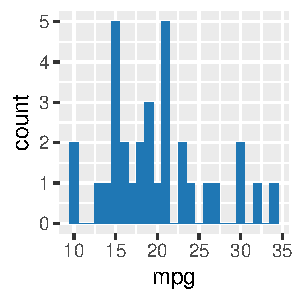
\includegraphics[width=0.5\linewidth]{Figs/unnamed-chunk-40-1} \end{center}
\end{frame}

\begin{frame}{Coordinates}
\phantomsection\label{coordinates-9}
We can set the aspect ratio of a plot with \(coord\_fixed()\), which
uses \(ratio = 1\) as a default.

A \(1:1\) aspect ratio is most appropriate when two continuous variables
are on the same scale, as with the iris dataset.
\end{frame}

\begin{frame}{Coordinates}
\phantomsection\label{coordinates-10}
All variables are measured in centimeters, so it only makes sense that
one unit on the plot should be the same physical distance on each axis.

This gives a more truthful depiction of the relationship between the two
variables since the aspect ratio can change the angle of our smoothing
line.
\end{frame}

\begin{frame}{Coordinates}
\phantomsection\label{coordinates-11}
This would give an erroneous impression of the data. Of course the
underlying linear models don't change, but our perception can be
influenced by the angle drawn.
\end{frame}

\begin{frame}{Coordinates}
\phantomsection\label{coordinates-12}
A plot using the iris dataset, of \textbf{sepal width} vs.~\textbf{sepal
length} colored by species, is shown in the viewer.
\end{frame}

\begin{frame}[fragile]{Aspect ratio I: 1:1 ratios}
\phantomsection\label{aspect-ratio-i-11-ratios}
Add a fixed coordinate layer to force a 1:1 aspect ratio.

\AddToHookNext{env/Highlighting/begin}{\tiny}

\begin{Shaded}
\begin{Highlighting}[]
\FunctionTok{ggplot}\NormalTok{(iris, }\FunctionTok{aes}\NormalTok{(}\AttributeTok{x =}\NormalTok{ Sepal.Length, }\AttributeTok{y =}\NormalTok{ Sepal.Width, }\AttributeTok{color =}\NormalTok{ Species)) }\SpecialCharTok{+}
    \FunctionTok{geom\_jitter}\NormalTok{() }\SpecialCharTok{+} \FunctionTok{geom\_smooth}\NormalTok{(}\AttributeTok{method =} \StringTok{"lm"}\NormalTok{, }\AttributeTok{se =} \ConstantTok{FALSE}\NormalTok{) }\SpecialCharTok{+}
    \FunctionTok{coord\_fixed}\NormalTok{()  }\CommentTok{\# Fix the coordinate ratio}
\end{Highlighting}
\end{Shaded}

\begin{center}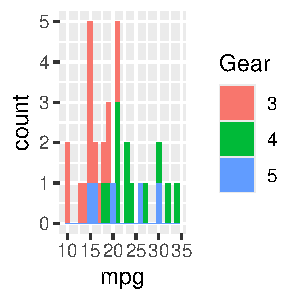
\includegraphics[width=0.5\linewidth]{Figs/unnamed-chunk-41-1} \end{center}
\end{frame}

\begin{frame}{Aspect ratio II}
\phantomsection\label{aspect-ratio-ii}
\begin{itemize}
\item
  setting ratios When values are not on the same scale it can be a bit
  tricky to set an appropriate aspect ratio.
\item
  A classic William Cleveland (inventor of dot plots) example is the
  sunspots data set. We have 3200 observations from 1750 to 2016.
\end{itemize}
\end{frame}

\begin{frame}[fragile]{Aspect ratio II}
\phantomsection\label{aspect-ratio-ii-1}
\begin{itemize}
\tightlist
\item
  \(sun\_plot\) is a plot without any set aspect ratio.
\end{itemize}

\AddToHookNext{env/Highlighting/begin}{\tiny}

\begin{Shaded}
\begin{Highlighting}[]
\FunctionTok{library}\NormalTok{(reshape2)}
\FunctionTok{library}\NormalTok{(zoo)}
\NormalTok{sunspots.m }\OtherTok{\textless{}{-}} \FunctionTok{data.frame}\NormalTok{(}\AttributeTok{year =} \FunctionTok{index}\NormalTok{(sunspot.month), }\AttributeTok{value =} \FunctionTok{melt}\NormalTok{(sunspot.month)}\SpecialCharTok{$}\NormalTok{value)}
\NormalTok{sun\_plot }\OtherTok{\textless{}{-}} \FunctionTok{ggplot}\NormalTok{(sunspots.m, }\FunctionTok{aes}\NormalTok{(}\AttributeTok{x =}\NormalTok{ year, }\AttributeTok{y =}\NormalTok{ value)) }\SpecialCharTok{+} \FunctionTok{geom\_line}\NormalTok{()}
\end{Highlighting}
\end{Shaded}

\begin{itemize}
\tightlist
\item
  It fills up the graphics device.
\end{itemize}
\end{frame}

\begin{frame}[fragile]{Aspect ratio II}
\phantomsection\label{aspect-ratio-ii-2}
\begin{itemize}
\tightlist
\item
  To make aspect ratios clear, we've drawn an orange box that is 75
  units high and 75 years wide.
\end{itemize}

\AddToHookNext{env/Highlighting/begin}{\tiny}

\begin{Shaded}
\begin{Highlighting}[]
\FunctionTok{library}\NormalTok{(reshape2)}
\FunctionTok{library}\NormalTok{(zoo)}
\NormalTok{sunspots.m }\OtherTok{\textless{}{-}} \FunctionTok{data.frame}\NormalTok{(}\AttributeTok{year =} \FunctionTok{index}\NormalTok{(sunspot.month), }\AttributeTok{value =} \FunctionTok{melt}\NormalTok{(sunspot.month)}\SpecialCharTok{$}\NormalTok{value)}
\NormalTok{sun\_plot }\OtherTok{\textless{}{-}} \FunctionTok{ggplot}\NormalTok{(sunspots.m, }\FunctionTok{aes}\NormalTok{(}\AttributeTok{x =}\NormalTok{ year, }\AttributeTok{y =}\NormalTok{ value)) }\SpecialCharTok{+} \FunctionTok{geom\_line}\NormalTok{() }\SpecialCharTok{+}
    \FunctionTok{coord\_fixed}\NormalTok{()}
\end{Highlighting}
\end{Shaded}

\begin{itemize}
\tightlist
\item
  Using a \(1:1\) aspect ratio would make the box square.
\end{itemize}
\end{frame}

\begin{frame}{Aspect ratio II}
\phantomsection\label{aspect-ratio-ii-3}
That aspect ratio would make things harder to see the oscillations: it
is better to force a wider ratio.
\end{frame}

\begin{frame}[fragile]{Aspect ratio II}
\phantomsection\label{aspect-ratio-ii-4}
Fix the coordinates to a 1:1 aspect ratio. The y axis is now unreadably
small. Make it bigger!

\AddToHookNext{env/Highlighting/begin}{\tiny}

\begin{Shaded}
\begin{Highlighting}[]
\CommentTok{\# Fix the aspect ratio to 1:1}
\NormalTok{sun\_plot }\SpecialCharTok{+} \FunctionTok{coord\_fixed}\NormalTok{()}
\end{Highlighting}
\end{Shaded}

\begin{center}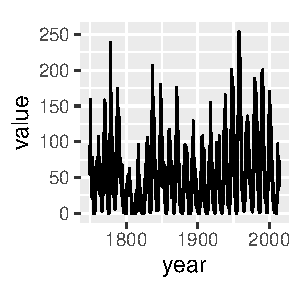
\includegraphics[width=0.5\linewidth]{Figs/unnamed-chunk-44-1} \end{center}
\end{frame}

\begin{frame}[fragile]{Aspect ratio II}
\phantomsection\label{aspect-ratio-ii-5}
\begin{itemize}
\item
  Change the aspect ratio to \(20:1\).
\item
  This is the aspect ratio recommended by Cleveland to help make the
  trend among oscillations easiest to see. \# Fix the aspect ratio to
  1:1
\end{itemize}

\AddToHookNext{env/Highlighting/begin}{\tiny}

\begin{Shaded}
\begin{Highlighting}[]
\CommentTok{\# Change the aspect ratio to 20:1}
\NormalTok{sun\_plot }\SpecialCharTok{+} \FunctionTok{coord\_fixed}\NormalTok{(}\AttributeTok{ratio =} \DecValTok{20}\NormalTok{)}
\end{Highlighting}
\end{Shaded}

\begin{center}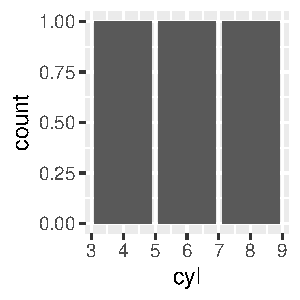
\includegraphics[width=0.5\linewidth]{Figs/unnamed-chunk-45-1} \end{center}
\end{frame}

\begin{frame}{Expand and clip}
\phantomsection\label{expand-and-clip}
The \(coord\_\star()\) layer functions offer two useful arguments that
work well together: expand and clip.
\end{frame}

\begin{frame}{Expand and clip}
\phantomsection\label{expand-and-clip-1}
\textbf{expand} sets a buffer margin around the plot, so data and axes
don't overlap.

Setting expand to 0 draws the axes to the limits of the data.
\end{frame}

\begin{frame}{Expand and clip}
\phantomsection\label{expand-and-clip-2}
clip decides whether plot elements that would lie outside the plot panel
are displayed or ignored (``clipped'').

When done properly this can make a great visual effect! We'll use
theme\_classic() and modify the axis lines in this example.
\end{frame}

\begin{frame}[fragile]{Expand and clip}
\phantomsection\label{expand-and-clip-3}
Add Cartesian coordinates with zero expansion, to remove all buffer
margins on both the x and y axes.

\AddToHookNext{env/Highlighting/begin}{\tiny}

\begin{Shaded}
\begin{Highlighting}[]
\FunctionTok{ggplot}\NormalTok{(mtcars, }\FunctionTok{aes}\NormalTok{(wt, mpg)) }\SpecialCharTok{+} \FunctionTok{geom\_point}\NormalTok{(}\AttributeTok{size =} \DecValTok{2}\NormalTok{) }\SpecialCharTok{+} \FunctionTok{theme\_classic}\NormalTok{() }\SpecialCharTok{+}
    \FunctionTok{coord\_cartesian}\NormalTok{(}\AttributeTok{expand =} \DecValTok{0}\NormalTok{)}
\end{Highlighting}
\end{Shaded}

\begin{center}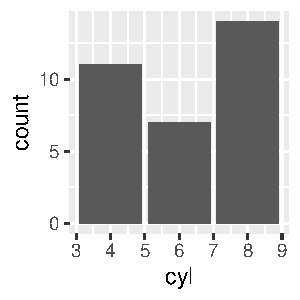
\includegraphics[width=0.5\linewidth]{Figs/unnamed-chunk-46-1} \end{center}

Setting expand to 0 caused points at the edge of the plot panel to be
cut off.
\end{frame}

\begin{frame}[fragile]{Expand and clip}
\phantomsection\label{expand-and-clip-4}
Set the clip argument to ``off'' to prevent this.

Remove the axis lines by setting the axis.line argument to
element\_blank() in the theme() layer function.

\AddToHookNext{env/Highlighting/begin}{\tiny}

\begin{Shaded}
\begin{Highlighting}[]
\FunctionTok{ggplot}\NormalTok{(mtcars, }\FunctionTok{aes}\NormalTok{(wt, mpg)) }\SpecialCharTok{+} \FunctionTok{geom\_point}\NormalTok{(}\AttributeTok{size =} \DecValTok{2}\NormalTok{) }\SpecialCharTok{+} \FunctionTok{coord\_cartesian}\NormalTok{(}\AttributeTok{expand =} \DecValTok{0}\NormalTok{,}
    \AttributeTok{clip =} \StringTok{"off"}\NormalTok{) }\SpecialCharTok{+} \FunctionTok{theme\_classic}\NormalTok{() }\SpecialCharTok{+} \FunctionTok{theme}\NormalTok{(}\AttributeTok{axis.line =} \FunctionTok{element\_blank}\NormalTok{())  }\CommentTok{\# Remove axis lines}
\end{Highlighting}
\end{Shaded}

\begin{center}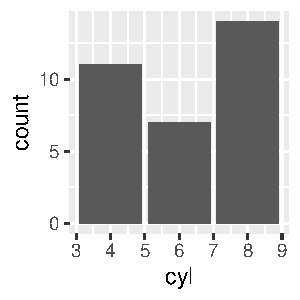
\includegraphics[width=0.5\linewidth]{Figs/unnamed-chunk-47-1} \end{center}
\end{frame}

\begin{frame}{Coordinates vs.~scales}
\phantomsection\label{coordinates-vs.-scales}
Log-transforming scales Using \(scale\_y\_log10()\) and
\(scale\_x\_log10()\) is equivalent to transforming our actual dataset
before getting to ggplot2.
\end{frame}

\begin{frame}{Coordinates vs.~scales}
\phantomsection\label{coordinates-vs.-scales-1}
Using \(coord\_trans()\), setting \(x = "log10"\) and/or \(y = "log10"\)
arguments, transforms the data after statistics have been calculated.
\end{frame}

\begin{frame}{Coordinates vs.~scales}
\phantomsection\label{coordinates-vs.-scales-2}
The plot will look the same as with using \(scale\_y\_log10()\), but the
scales will be different, meaning that we'll see the original values on
our log10 transformed axes.
\end{frame}

\begin{frame}{Coordinates vs.~scales}
\phantomsection\label{coordinates-vs.-scales-3}
This can be useful since log scales can be somewhat unintuitive.

Let's see this in action with positively skewed data - the brain and
body weight of 51 mammals from the msleep dataset.
\end{frame}

\begin{frame}[fragile]{Coordinates vs.~scales}
\phantomsection\label{coordinates-vs.-scales-4}
Using the msleep dataset, plot the raw values of brainwt against bodywt
values as a scatter plot.

\AddToHookNext{env/Highlighting/begin}{\tiny}

\begin{Shaded}
\begin{Highlighting}[]
\CommentTok{\# Produce a scatter plot of brainwt vs. bodywt}
\FunctionTok{ggplot}\NormalTok{(msleep, }\FunctionTok{aes}\NormalTok{(bodywt, brainwt)) }\SpecialCharTok{+} \FunctionTok{geom\_point}\NormalTok{() }\SpecialCharTok{+} \FunctionTok{ggtitle}\NormalTok{(}\StringTok{"Raw Values"}\NormalTok{)}
\end{Highlighting}
\end{Shaded}

\begin{center}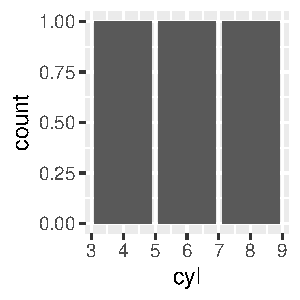
\includegraphics[width=0.5\linewidth]{Figs/unnamed-chunk-48-1} \end{center}
\end{frame}

\begin{frame}[fragile]{Coordinates vs.~scales}
\phantomsection\label{coordinates-vs.-scales-5}
Add the \(scale\_x\_log10()\) and \(scale\_y\_log10()\) layers with
default values to transform the data before plotting.

\AddToHookNext{env/Highlighting/begin}{\tiny}

\begin{Shaded}
\begin{Highlighting}[]
\CommentTok{\# Add scale\_*\_*() functions}
\FunctionTok{ggplot}\NormalTok{(msleep, }\FunctionTok{aes}\NormalTok{(bodywt, brainwt)) }\SpecialCharTok{+} \FunctionTok{geom\_point}\NormalTok{() }\SpecialCharTok{+} \FunctionTok{scale\_x\_log10}\NormalTok{() }\SpecialCharTok{+}
    \FunctionTok{scale\_y\_log10}\NormalTok{() }\SpecialCharTok{+} \FunctionTok{ggtitle}\NormalTok{(}\StringTok{"Scale\_ functions"}\NormalTok{)}
\end{Highlighting}
\end{Shaded}

\begin{center}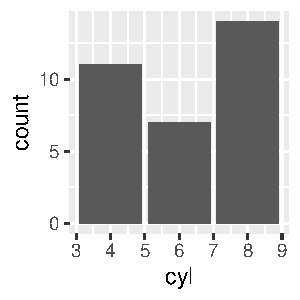
\includegraphics[width=0.5\linewidth]{Figs/unnamed-chunk-49-1} \end{center}
\end{frame}

\begin{frame}[fragile]{Coordinates vs.~scales}
\phantomsection\label{coordinates-vs.-scales-6}
Use coord\_trans() to apply a ``log10'' transformation to both the x and
y scales

\AddToHookNext{env/Highlighting/begin}{\tiny}

\begin{Shaded}
\begin{Highlighting}[]
\CommentTok{\# Perform a log10 coordinate system transformation}
\FunctionTok{ggplot}\NormalTok{(msleep, }\FunctionTok{aes}\NormalTok{(bodywt, brainwt)) }\SpecialCharTok{+} \FunctionTok{geom\_point}\NormalTok{() }\SpecialCharTok{+} \FunctionTok{coord\_trans}\NormalTok{(}\AttributeTok{x =} \StringTok{"log10"}\NormalTok{,}
    \AttributeTok{y =} \StringTok{"log10"}\NormalTok{)}
\end{Highlighting}
\end{Shaded}

\begin{center}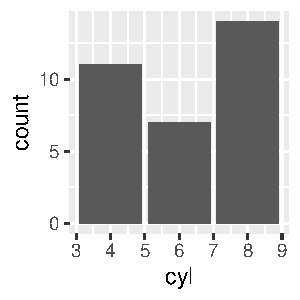
\includegraphics[width=0.5\linewidth]{Figs/unnamed-chunk-50-1} \end{center}
\end{frame}

\begin{frame}{Adding stats to transformed scales}
\phantomsection\label{adding-stats-to-transformed-scales}
In the last exercise, we saw the usefulness of the coord\_trans()
function, but be careful!

Remember that statistics are calculated on the untransformed data.
\end{frame}

\begin{frame}{Adding stats to transformed scales}
\phantomsection\label{adding-stats-to-transformed-scales-1}
A linear model may end up looking not-so-linear after an axis
transformation.

Let's revisit the two plots from the previous exercise and compare their
linear models.
\end{frame}

\begin{frame}[fragile]{Adding stats to transformed scales}
\phantomsection\label{adding-stats-to-transformed-scales-2}
Add log10 transformed scales to the x and y axes.

\AddToHookNext{env/Highlighting/begin}{\tiny}

\begin{Shaded}
\begin{Highlighting}[]
\CommentTok{\# Plot with a scale\_*\_*() function:}
\FunctionTok{ggplot}\NormalTok{(msleep, }\FunctionTok{aes}\NormalTok{(bodywt, brainwt)) }\SpecialCharTok{+}
  \FunctionTok{geom\_point}\NormalTok{() }\SpecialCharTok{+}
  \FunctionTok{geom\_smooth}\NormalTok{(}\AttributeTok{method =} \StringTok{"lm"}\NormalTok{, }\AttributeTok{se =} \ConstantTok{FALSE}\NormalTok{) }\SpecialCharTok{+}
  \FunctionTok{scale\_x\_log10}\NormalTok{() }\SpecialCharTok{+} \CommentTok{\# Add a log10 x scale}
  \FunctionTok{scale\_y\_log10}\NormalTok{() }\SpecialCharTok{+} \CommentTok{\# Add a log10 y scale}
  \FunctionTok{ggtitle}\NormalTok{(}\StringTok{"Scale\_ functions"}\NormalTok{)}
\end{Highlighting}
\end{Shaded}

\begin{center}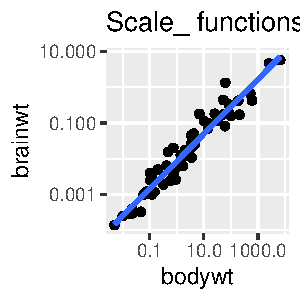
\includegraphics[width=0.5\linewidth]{Figs/unnamed-chunk-51-1} \end{center}

Do you notice the difference between the two plots?
\end{frame}

\begin{frame}[fragile]{Adding stats to transformed scales}
\phantomsection\label{adding-stats-to-transformed-scales-3}
Plot with transformed coordinates

\AddToHookNext{env/Highlighting/begin}{\tiny}

\begin{Shaded}
\begin{Highlighting}[]
\CommentTok{\# Plot with transformed coordinates}
\FunctionTok{ggplot}\NormalTok{(msleep, }\FunctionTok{aes}\NormalTok{(bodywt, brainwt)) }\SpecialCharTok{+}
  \FunctionTok{geom\_point}\NormalTok{() }\SpecialCharTok{+}
  \FunctionTok{geom\_smooth}\NormalTok{(}\AttributeTok{method =} \StringTok{"lm"}\NormalTok{, }\AttributeTok{se =} \ConstantTok{FALSE}\NormalTok{) }\SpecialCharTok{+} \CommentTok{\# Add a log10 coordinate transformation for x and y axes}
  \FunctionTok{coord\_trans}\NormalTok{(}\AttributeTok{x =} \StringTok{"log10"}\NormalTok{, }\AttributeTok{y =} \StringTok{"log10"}\NormalTok{)}
\end{Highlighting}
\end{Shaded}

\begin{center}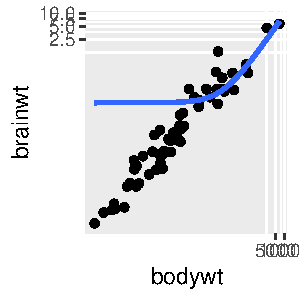
\includegraphics[width=0.5\linewidth]{Figs/unnamed-chunk-52-1} \end{center}
\end{frame}

\begin{frame}{Double and flipped axes}
\phantomsection\label{double-and-flipped-axes}
\begin{itemize}
\item
  Useful double axes Double x and y-axes are a contentious topic in data
  visualization.
\item
  Here, I want to review a great use case where double axes actually do
  add value to a plot.
\end{itemize}
\end{frame}

\begin{frame}[fragile]{Double and flipped axes}
\phantomsection\label{double-and-flipped-axes-1}
Our goal plot is displayed in the viewer.

\AddToHookNext{env/Highlighting/begin}{\tiny}

\begin{Shaded}
\begin{Highlighting}[]
\FunctionTok{library}\NormalTok{(lubridate)}
\NormalTok{airquality }\OtherTok{\textless{}{-}}\NormalTok{ airquality }\SpecialCharTok{\%\textgreater{}\%}
    \FunctionTok{mutate}\NormalTok{(}\AttributeTok{Date =} \FunctionTok{make\_date}\NormalTok{(}\DecValTok{1974}\NormalTok{, Month, Day))}
\end{Highlighting}
\end{Shaded}
\end{frame}

\begin{frame}{Double and flipped axes}
\phantomsection\label{double-and-flipped-axes-2}
The two axes are the raw temperature values on a Fahrenheit scale and
the transformed values on a Celsius scale.

You can imagine a similar scenario for Log-transformed and original
values, miles and kilometers, or pounds and kilograms.
\end{frame}

\begin{frame}{Double and flipped axes}
\phantomsection\label{double-and-flipped-axes-3}
A scale that is unintuitive for many people can be made easier by adding
a transformation as a double axis.
\end{frame}

\begin{frame}[fragile]{Double and flipped axes}
\phantomsection\label{double-and-flipped-axes-4}
Begin with a standard line plot, of Temp described by Date in the
airquality dataset.

\AddToHookNext{env/Highlighting/begin}{\tiny}

\begin{Shaded}
\begin{Highlighting}[]
\CommentTok{\# Using airquality, plot Temp vs. Date}
\FunctionTok{ggplot}\NormalTok{(airquality, }\FunctionTok{aes}\NormalTok{(}\AttributeTok{x =}\NormalTok{ Date, }\AttributeTok{y =}\NormalTok{ Temp)) }\SpecialCharTok{+}
  \FunctionTok{geom\_line}\NormalTok{() }\SpecialCharTok{+} \CommentTok{\# Add a line layer}
  \FunctionTok{labs}\NormalTok{(}\AttributeTok{x =} \StringTok{"Date (1973)"}\NormalTok{, }\AttributeTok{y =} \StringTok{"Fahrenheit"}\NormalTok{)}
\end{Highlighting}
\end{Shaded}

\begin{center}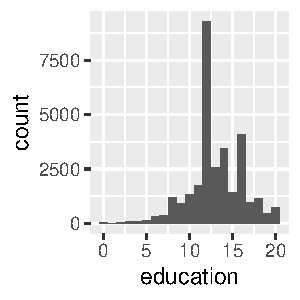
\includegraphics[width=0.5\linewidth]{Figs/unnamed-chunk-54-1} \end{center}
\end{frame}

\begin{frame}[fragile]{Double and flipped axes}
\phantomsection\label{double-and-flipped-axes-5}
Convert y\_breaks from Fahrenheit to Celsius (subtract 32, then multiply
by 5, then divide by 9).

\AddToHookNext{env/Highlighting/begin}{\tiny}

\begin{Shaded}
\begin{Highlighting}[]
\CommentTok{\# Define breaks (Fahrenheit)}
\NormalTok{y\_breaks }\OtherTok{\textless{}{-}} \FunctionTok{c}\NormalTok{(}\DecValTok{59}\NormalTok{, }\DecValTok{68}\NormalTok{, }\DecValTok{77}\NormalTok{, }\DecValTok{86}\NormalTok{, }\DecValTok{95}\NormalTok{, }\DecValTok{104}\NormalTok{)}

\CommentTok{\# Convert y\_breaks from Fahrenheit to Celsius}
\NormalTok{y\_labels }\OtherTok{\textless{}{-}}\NormalTok{ (y\_breaks }\SpecialCharTok{{-}} \DecValTok{32}\NormalTok{) }\SpecialCharTok{*} \DecValTok{5}\SpecialCharTok{/}\DecValTok{9}
\end{Highlighting}
\end{Shaded}
\end{frame}

\begin{frame}[fragile]{Double and flipped axes}
\phantomsection\label{double-and-flipped-axes-6}
Define the secondary y-axis using sec\_axis(). Use the identity
transformation. Set the breaks and labels to the defined objects
y\_breaks and y\_labels, respectively.

\AddToHookNext{env/Highlighting/begin}{\tiny}

\begin{Shaded}
\begin{Highlighting}[]
\CommentTok{\# Create a secondary x{-}axis}
\NormalTok{secondary\_y\_axis }\OtherTok{\textless{}{-}} \FunctionTok{sec\_axis}\NormalTok{(}
  \CommentTok{\# Use identity transformation}
  \AttributeTok{trans =}\NormalTok{ identity,}
  \AttributeTok{name =} \StringTok{"Celsius"}\NormalTok{,}
  \CommentTok{\# Define breaks and labels as above}
  \AttributeTok{breaks =}\NormalTok{ y\_breaks,}
  \AttributeTok{labels =}\NormalTok{ y\_labels}
\NormalTok{)}

\CommentTok{\# Examine the object}
\NormalTok{secondary\_y\_axis}
\end{Highlighting}
\end{Shaded}

\begin{verbatim}
<ggproto object: Class AxisSecondary, gg>
    axis: NULL
    break_info: function
    breaks: 59 68 77 86 95 104
    create_scale: function
    detail: 1000
    empty: function
    guide: waiver
    init: function
    labels: 15 20 25 30 35 40
    make_title: function
    mono_test: function
    name: Celsius
    trans: function
    transform_range: function
    super:  <ggproto object: Class AxisSecondary, gg>
\end{verbatim}
\end{frame}

\begin{frame}[fragile]{Double and flipped axes}
\phantomsection\label{double-and-flipped-axes-7}
Add your secondary y-axis to the sec.axis argument of
\(scale\_y\_continuous()\).

\AddToHookNext{env/Highlighting/begin}{\tiny}

\begin{Shaded}
\begin{Highlighting}[]
\CommentTok{\# From previous step}
\NormalTok{y\_breaks }\OtherTok{\textless{}{-}} \FunctionTok{c}\NormalTok{(}\DecValTok{59}\NormalTok{, }\DecValTok{68}\NormalTok{, }\DecValTok{77}\NormalTok{, }\DecValTok{86}\NormalTok{, }\DecValTok{95}\NormalTok{, }\DecValTok{104}\NormalTok{)}
\NormalTok{y\_labels }\OtherTok{\textless{}{-}}\NormalTok{ (y\_breaks }\SpecialCharTok{{-}} \DecValTok{32}\NormalTok{) }\SpecialCharTok{*} \DecValTok{5}\SpecialCharTok{/}\DecValTok{9}
\NormalTok{secondary\_y\_axis }\OtherTok{\textless{}{-}} \FunctionTok{sec\_axis}\NormalTok{(}\AttributeTok{trans =}\NormalTok{ identity, }\AttributeTok{name =} \StringTok{"Celsius"}\NormalTok{,}
    \AttributeTok{breaks =}\NormalTok{ y\_breaks, }\AttributeTok{labels =}\NormalTok{ y\_labels)}
\end{Highlighting}
\end{Shaded}
\end{frame}

\begin{frame}[fragile]{Update the plot}
\phantomsection\label{update-the-plot}
\AddToHookNext{env/Highlighting/begin}{\tiny}

\begin{Shaded}
\begin{Highlighting}[]
\CommentTok{\# Update the plot}
\FunctionTok{ggplot}\NormalTok{(airquality, }\FunctionTok{aes}\NormalTok{(}\AttributeTok{x =}\NormalTok{ Date, }\AttributeTok{y =}\NormalTok{ Temp)) }\SpecialCharTok{+}
  \FunctionTok{geom\_line}\NormalTok{() }\SpecialCharTok{+}
  \FunctionTok{scale\_y\_continuous}\NormalTok{(}\AttributeTok{sec.axis =}\NormalTok{ secondary\_y\_axis) }\SpecialCharTok{+} \CommentTok{\# Add the secondary y{-}axis }
  \FunctionTok{labs}\NormalTok{(}\AttributeTok{x =} \StringTok{"Date (1973)"}\NormalTok{, }\AttributeTok{y =} \StringTok{"Fahrenheit"}\NormalTok{)}
\end{Highlighting}
\end{Shaded}

\begin{center}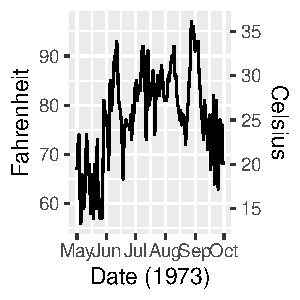
\includegraphics[width=0.5\linewidth]{Figs/unnamed-chunk-58-1} \end{center}
\end{frame}

\begin{frame}{Flipping axes I}
\phantomsection\label{flipping-axes-i}
Flipping axes means to reverse the variables mapped onto the x and y
aesthetics.

We can just change the mappings in \(aes()\), but we can also use the
\(coord\_flip()\) layer function.

There are two reasons to use this function:
\end{frame}

\begin{frame}{Flipping axes I}
\phantomsection\label{flipping-axes-i-1}
We want a vertical geom to be horizontal, or We've completed a long
series of plotting functions and want to flip it without having to
rewrite all our commands.
\end{frame}

\begin{frame}[fragile]{Flipping axes I}
\phantomsection\label{flipping-axes-i-2}
Create a side-by-side (``dodged'') bar chart of fcyl, filled according
to fam.

\AddToHookNext{env/Highlighting/begin}{\tiny}

\begin{Shaded}
\begin{Highlighting}[]
\CommentTok{\# Plot fcyl bars, filled by fam}
\FunctionTok{ggplot}\NormalTok{(mtcars, }\FunctionTok{aes}\NormalTok{(fcyl, }\AttributeTok{fill =}\NormalTok{ fam)) }\SpecialCharTok{+} \CommentTok{\# Place bars side by side}
  \FunctionTok{geom\_bar}\NormalTok{(}\AttributeTok{position =} \StringTok{"dodge"}\NormalTok{)}
\end{Highlighting}
\end{Shaded}

\begin{center}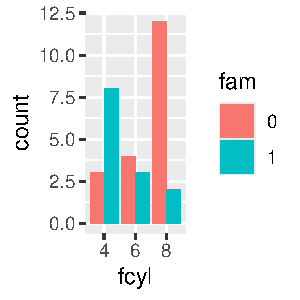
\includegraphics[width=0.5\linewidth]{Figs/unnamed-chunk-59-1} \end{center}
\end{frame}

\begin{frame}[fragile]{Flipping axes I}
\phantomsection\label{flipping-axes-i-3}
To get horizontal bars, add a \(coord\_flip()\) function.

\AddToHookNext{env/Highlighting/begin}{\tiny}

\begin{Shaded}
\begin{Highlighting}[]
\FunctionTok{ggplot}\NormalTok{(mtcars, }\FunctionTok{aes}\NormalTok{(fcyl, }\AttributeTok{fill =}\NormalTok{ fam)) }\SpecialCharTok{+}
  \FunctionTok{geom\_bar}\NormalTok{(}\AttributeTok{position =} \StringTok{"dodge"}\NormalTok{) }\SpecialCharTok{+} \CommentTok{\# Flip the x and y coordinates}
  \FunctionTok{coord\_flip}\NormalTok{()}
\end{Highlighting}
\end{Shaded}

\begin{center}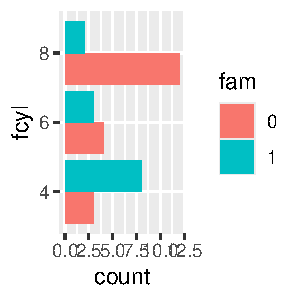
\includegraphics[width=0.5\linewidth]{Figs/unnamed-chunk-60-1} \end{center}
\end{frame}

\begin{frame}[fragile]{Flipping axes I}
\phantomsection\label{flipping-axes-i-4}
Partially overlapping bars are popular with ``infoviz'' in magazines.

Update the position argument to use \(position\_dodge()\) with a width
of 0.5.

\AddToHookNext{env/Highlighting/begin}{\tiny}

\begin{Shaded}
\begin{Highlighting}[]
\FunctionTok{ggplot}\NormalTok{(mtcars, }\FunctionTok{aes}\NormalTok{(fcyl, }\AttributeTok{fill =}\NormalTok{ fam)) }\SpecialCharTok{+}  \CommentTok{\# Set a dodge width of 0.5 for partially overlapping bars}
  \FunctionTok{geom\_bar}\NormalTok{(}\AttributeTok{position =} \FunctionTok{position\_dodge}\NormalTok{(}\FloatTok{0.5}\NormalTok{)) }\SpecialCharTok{+}
  \FunctionTok{coord\_flip}\NormalTok{()}
\end{Highlighting}
\end{Shaded}

\begin{center}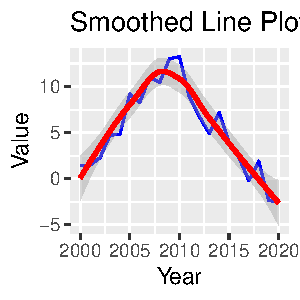
\includegraphics[width=0.5\linewidth]{Figs/unnamed-chunk-61-1} \end{center}
\end{frame}

\begin{frame}{Flipping axes II}
\phantomsection\label{flipping-axes-ii}
In this exercise, we'll continue to use the \(coord\_flip()\) layer
function to reverse the variables mapped onto the x and y aesthetics.
\end{frame}

\begin{frame}[fragile]{Flipping axes II}
\phantomsection\label{flipping-axes-ii-1}
Within the \textbf{mtcars} dataset, \textbf{car} is the name of the car
and \textbf{wt} is its weight.

\AddToHookNext{env/Highlighting/begin}{\tiny}

\begin{Shaded}
\begin{Highlighting}[]
\CommentTok{\# Add car names as a column}
\NormalTok{mtcars }\OtherTok{\textless{}{-}}\NormalTok{ mtcars }\SpecialCharTok{\%\textgreater{}\%}
    \FunctionTok{mutate}\NormalTok{(}\AttributeTok{car =} \FunctionTok{rownames}\NormalTok{(mtcars), }\AttributeTok{fam =} \FunctionTok{as.factor}\NormalTok{(am), }\AttributeTok{fcyl =} \FunctionTok{as.factor}\NormalTok{(cyl),}
        \AttributeTok{fvs =} \FunctionTok{as.factor}\NormalTok{(vs))}
\end{Highlighting}
\end{Shaded}
\end{frame}

\begin{frame}[fragile]{Flipping axes II}
\phantomsection\label{flipping-axes-ii-2}
Create a scatter plot of wt versus car using the mtcars dataset.

\AddToHookNext{env/Highlighting/begin}{\tiny}

\begin{Shaded}
\begin{Highlighting}[]
\CommentTok{\# Plot of wt vs. car}
\FunctionTok{ggplot}\NormalTok{(mtcars, }\FunctionTok{aes}\NormalTok{(car, wt)) }\SpecialCharTok{+} \FunctionTok{geom\_point}\NormalTok{() }\SpecialCharTok{+} \FunctionTok{labs}\NormalTok{(}\AttributeTok{x =} \StringTok{"car"}\NormalTok{,}
    \AttributeTok{y =} \StringTok{"weight"}\NormalTok{)}
\end{Highlighting}
\end{Shaded}

\begin{center}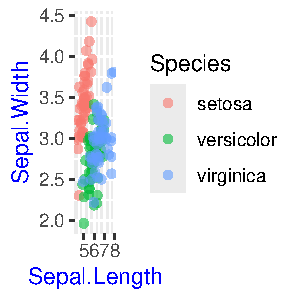
\includegraphics[width=0.5\linewidth]{Figs/unnamed-chunk-63-1} \end{center}
\end{frame}

\begin{frame}{Flipping axes II}
\phantomsection\label{flipping-axes-ii-3}
We'll flip the axes in the next step.

It would be easier to read if car was mapped to the y axis.
\end{frame}

\begin{frame}[fragile]{Flipping axes II}
\phantomsection\label{flipping-axes-ii-4}
Flip the coordinates. Notice that the labels also get flipped!

\AddToHookNext{env/Highlighting/begin}{\tiny}

\begin{Shaded}
\begin{Highlighting}[]
\CommentTok{\# Flip the axes to set car to the y axis}
\FunctionTok{ggplot}\NormalTok{(mtcars, }\FunctionTok{aes}\NormalTok{(car, wt)) }\SpecialCharTok{+} \FunctionTok{geom\_point}\NormalTok{() }\SpecialCharTok{+} \FunctionTok{labs}\NormalTok{(}\AttributeTok{x =} \StringTok{"car"}\NormalTok{,}
    \AttributeTok{y =} \StringTok{"weight"}\NormalTok{) }\SpecialCharTok{+} \FunctionTok{coord\_flip}\NormalTok{()}
\end{Highlighting}
\end{Shaded}

\begin{center}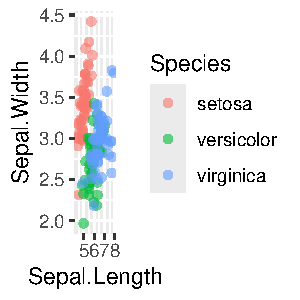
\includegraphics[width=0.5\linewidth]{Figs/unnamed-chunk-64-1} \end{center}
\end{frame}

\begin{frame}{Polar coordinates}
\phantomsection\label{polar-coordinates}
\textbf{Pie charts}

The \(coord\_polar()\) function converts a planar x-y Cartesian plot to
polar coordinates.

This can be useful if you are producing pie charts.
\end{frame}

\begin{frame}{Polar coordinates}
\phantomsection\label{polar-coordinates-1}
We can imagine two forms for pie charts - the typical filled circle, or
a colored ring.
\end{frame}

\begin{frame}{Polar coordinates}
\phantomsection\label{polar-coordinates-2}
Typical pie charts omit all of the non-data ink, which we saw in the
themes previously.

Pie charts are not really better than stacked bar charts, but we'll come
back to this point in the next chapter.
\end{frame}

\begin{frame}[fragile]{Polar coordinates}
\phantomsection\label{polar-coordinates-3}
A bar plot using mtcars of the number of cylinders (as a factor), fcyl,
is shown below.

\AddToHookNext{env/Highlighting/begin}{\tiny}

\begin{Shaded}
\begin{Highlighting}[]
\CommentTok{\# Run the code, view the plot, then update it}
\FunctionTok{ggplot}\NormalTok{(mtcars, }\FunctionTok{aes}\NormalTok{(}\AttributeTok{x =} \DecValTok{1}\NormalTok{, }\AttributeTok{fill =}\NormalTok{ fcyl)) }\SpecialCharTok{+} \FunctionTok{geom\_bar}\NormalTok{()}
\end{Highlighting}
\end{Shaded}

\begin{center}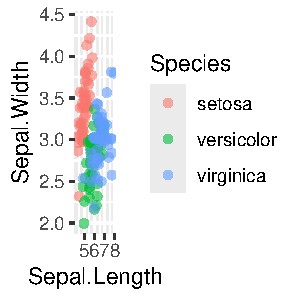
\includegraphics[width=0.5\linewidth]{Figs/unnamed-chunk-65-1} \end{center}

Run the code to see the stacked bar plot
\end{frame}

\begin{frame}[fragile]{Polar coordinates}
\phantomsection\label{polar-coordinates-4}
Add a polar coordinate system, mapping the angle to the y variable by
setting theta to ``y''.

\AddToHookNext{env/Highlighting/begin}{\tiny}

\begin{Shaded}
\begin{Highlighting}[]
\CommentTok{\# Run the code, view the plot, then update it}
\FunctionTok{ggplot}\NormalTok{(mtcars, }\FunctionTok{aes}\NormalTok{(}\AttributeTok{x =} \DecValTok{1}\NormalTok{, }\AttributeTok{fill =}\NormalTok{ fcyl)) }\SpecialCharTok{+} \FunctionTok{geom\_bar}\NormalTok{() }\SpecialCharTok{+} \FunctionTok{coord\_polar}\NormalTok{(}\AttributeTok{theta =} \StringTok{"y"}\NormalTok{)  }\CommentTok{\# Add a polar coordinate system}
\end{Highlighting}
\end{Shaded}

\begin{center}\includegraphics[width=0.5\linewidth]{Figs/unnamed-chunk-66-1} \end{center}
\end{frame}

\begin{frame}[fragile]{Polar coordinates}
\phantomsection\label{polar-coordinates-5}
Reduce the width of the bars to 0.1.

Make it a ring plot by adding a continuous x scale with limits from 0.5
to 1.5.

\AddToHookNext{env/Highlighting/begin}{\tiny}

\begin{Shaded}
\begin{Highlighting}[]
\FunctionTok{ggplot}\NormalTok{(mtcars, }\FunctionTok{aes}\NormalTok{(}\AttributeTok{x =} \DecValTok{1}\NormalTok{, }\AttributeTok{fill =}\NormalTok{ fcyl)) }\SpecialCharTok{+} \FunctionTok{geom\_bar}\NormalTok{(}\AttributeTok{width =} \FloatTok{0.1}\NormalTok{) }\SpecialCharTok{+}
    \FunctionTok{coord\_polar}\NormalTok{(}\AttributeTok{theta =} \StringTok{"y"}\NormalTok{) }\SpecialCharTok{+} \FunctionTok{scale\_x\_continuous}\NormalTok{(}\AttributeTok{limits =} \FunctionTok{c}\NormalTok{(}\FloatTok{0.5}\NormalTok{,}
    \FloatTok{1.5}\NormalTok{))  }\CommentTok{\# Add a continuous x scale from 0.5 to 1.5}
\end{Highlighting}
\end{Shaded}

\begin{center}\includegraphics[width=0.5\linewidth]{Figs/unnamed-chunk-67-1} \end{center}

Add a continuous x scale from 0.5 to 1.5
\end{frame}

\begin{frame}{Wind rose plots}
\phantomsection\label{wind-rose-plots}
\begin{itemize}
\item
  Polar coordinate plots are well-suited to scales like compass
  direction or time of day.
\item
  A popular example is the ``wind rose''.
\end{itemize}
\end{frame}

\begin{frame}[fragile]{Wind rose plots}
\phantomsection\label{wind-rose-plots-1}
The \textbf{mydata} dataset is taken from the openair package and
contains hourly measurements for windspeed (ws) and direction (wd) from
London in 2003.

\AddToHookNext{env/Highlighting/begin}{\tiny}

\begin{Shaded}
\begin{Highlighting}[]
\FunctionTok{library}\NormalTok{(openair)}
\CommentTok{\# Load wind data}
\FunctionTok{data}\NormalTok{(mydata)}

\CommentTok{\# Remove NA values}
\NormalTok{mydata }\OtherTok{\textless{}{-}} \FunctionTok{na.omit}\NormalTok{(mydata)}

\CommentTok{\# Bin wind speed into categories for better visualization}
\NormalTok{mydata }\OtherTok{\textless{}{-}}\NormalTok{ mydata }\SpecialCharTok{\%\textgreater{}\%}
    \FunctionTok{mutate}\NormalTok{(}\AttributeTok{ws\_bin =} \FunctionTok{cut}\NormalTok{(ws, }\AttributeTok{breaks =} \FunctionTok{seq}\NormalTok{(}\DecValTok{0}\NormalTok{, }\FunctionTok{max}\NormalTok{(ws, }\AttributeTok{na.rm =} \ConstantTok{TRUE}\NormalTok{),}
        \AttributeTok{by =} \DecValTok{1}\NormalTok{), }\AttributeTok{include.lowest =} \ConstantTok{TRUE}\NormalTok{))}
\CommentTok{\# Ensure wind direction (wd) is categorical}
\NormalTok{mydata}\SpecialCharTok{$}\NormalTok{wd }\OtherTok{\textless{}{-}} \FunctionTok{factor}\NormalTok{(mydata}\SpecialCharTok{$}\NormalTok{wd)}
\FunctionTok{head}\NormalTok{(mydata)}
\end{Highlighting}
\end{Shaded}

\begin{verbatim}
# A tibble: 6 x 11
  date                   ws wd      nox   no2    o3  pm10   so2    co  pm25
  <dttm>              <dbl> <fct> <int> <int> <int> <int> <dbl> <dbl> <int>
1 1998-05-01 07:00:00  3.6  350      81    37    13    24  2.90  0.81    16
2 1998-05-01 08:00:00  3.6  350     107    43    12    23  3.13  0.91    16
3 1998-05-01 09:00:00  3.6  340     127    34    11    21  3.1   1.18    15
4 1998-05-01 10:00:00  3    350     122    50    10    23  3.24  1.48    17
5 1998-05-01 11:00:00  3.6  350     115    37    12    25  3.24  1.16    18
6 1998-05-01 12:00:00  3.96 360     114    47    11    27  2.90  1.16    21
# i 1 more variable: ws_bin <fct>
\end{verbatim}

Both variables are factors.
\end{frame}

\begin{frame}[fragile]{Wind rose plots}
\phantomsection\label{wind-rose-plots-2}
Make a classic bar plot mapping \textbf{wd} onto the \textbf{x}
aesthetic and \textbf{ws} onto fill.

\AddToHookNext{env/Highlighting/begin}{\tiny}

\begin{Shaded}
\begin{Highlighting}[]
\CommentTok{\# Create a polar bar plot}
\FunctionTok{ggplot}\NormalTok{(mydata, }\FunctionTok{aes}\NormalTok{(}\AttributeTok{x =}\NormalTok{ wd, }\AttributeTok{fill =}\NormalTok{ ws\_bin)) }\SpecialCharTok{+} \FunctionTok{geom\_bar}\NormalTok{(}\AttributeTok{width =} \DecValTok{1}\NormalTok{)}
\end{Highlighting}
\end{Shaded}

\begin{center}\includegraphics[width=0.5\linewidth]{Figs/unnamed-chunk-69-1} \end{center}

Use a \(geom\_bar()\) layer, since we want to aggregate over all date
values, and set the width argument to 1, to eliminate any spaces between
the bars.
\end{frame}

\begin{frame}[fragile]{Wind rose plots}
\phantomsection\label{wind-rose-plots-3}
Convert the Cartesian coordinate space into a polar coordinate space
with \(coord\_polar()\).

\AddToHookNext{env/Highlighting/begin}{\tiny}

\begin{Shaded}
\begin{Highlighting}[]
\CommentTok{\# Convert to polar coordinates:}
\FunctionTok{ggplot}\NormalTok{(mydata, }\FunctionTok{aes}\NormalTok{(}\AttributeTok{x =}\NormalTok{ wd, }\AttributeTok{fill =}\NormalTok{ ws)) }\SpecialCharTok{+} 
  \FunctionTok{geom\_bar}\NormalTok{(}\AttributeTok{width =} \DecValTok{1}\NormalTok{) }\SpecialCharTok{+}  \CommentTok{\# Use bars with no spacing}
  \FunctionTok{coord\_polar}\NormalTok{()}
\end{Highlighting}
\end{Shaded}

\begin{center}\includegraphics[width=0.5\linewidth]{Figs/unnamed-chunk-70-1} \end{center}
\end{frame}

\begin{frame}[fragile]{Wind rose plots}
\phantomsection\label{wind-rose-plots-4}
Set the start argument to \(-\pi/16\) to position North at the top of
the plot.

\AddToHookNext{env/Highlighting/begin}{\tiny}

\begin{Shaded}
\begin{Highlighting}[]
\CommentTok{\# Create a polar bar plot}
\FunctionTok{ggplot}\NormalTok{(mydata, }\FunctionTok{aes}\NormalTok{(}\AttributeTok{x =}\NormalTok{ wd, }\AttributeTok{fill =}\NormalTok{ ws\_bin)) }\SpecialCharTok{+} 
  \FunctionTok{geom\_bar}\NormalTok{(}\AttributeTok{width =} \DecValTok{1}\NormalTok{) }\SpecialCharTok{+}  \CommentTok{\# Use bars with no spacing}
  \FunctionTok{coord\_polar}\NormalTok{(}\AttributeTok{start =} \SpecialCharTok{{-}}\NormalTok{pi}\SpecialCharTok{/}\DecValTok{16}\NormalTok{) }\SpecialCharTok{+}  \CommentTok{\# Convert to polar coordinates, with North at top}
  \FunctionTok{labs}\NormalTok{(}\AttributeTok{x =} \StringTok{"Wind Direction"}\NormalTok{, }\AttributeTok{y =} \StringTok{"Frequency"}\NormalTok{, }\AttributeTok{fill =} \StringTok{"Wind Speed"}\NormalTok{) }\SpecialCharTok{+}
  \FunctionTok{theme\_minimal}\NormalTok{() }\SpecialCharTok{+}
  \FunctionTok{theme}\NormalTok{(}\AttributeTok{axis.text.y =} \FunctionTok{element\_blank}\NormalTok{(),  }\CommentTok{\# Remove y{-}axis text for cleaner look}
        \AttributeTok{panel.grid =} \FunctionTok{element\_blank}\NormalTok{())   }\CommentTok{\# Remove grid for minimal appearance}
\end{Highlighting}
\end{Shaded}

\begin{center}\includegraphics[width=0.5\linewidth]{Figs/unnamed-chunk-71-1} \end{center}
\end{frame}

\section{Facets}\label{facets}

\begin{frame}{Facets}
\phantomsection\label{facets-1}
Facets let you split plots into multiple panes, each displaying subsets
of the dataset.

Here you'll learn how to wrap facets and arrange them in a grid, as well
as providing custom labeling.
\end{frame}

\begin{frame}[fragile]{Facet layer basics}
\phantomsection\label{facet-layer-basics}
Faceting splits the data up into groups, according to a categorical
variable, then plots each group in its own panel.

For splitting the data by one or two categorical variables,
\texttt{facet\_grid()} is best.
\end{frame}

\begin{frame}[fragile]{Facet layer basics}
\phantomsection\label{facet-layer-basics-1}
Given categorical variables \textbf{A} and \textbf{B}, the code pattern
is:

\AddToHookNext{env/Highlighting/begin}{\tiny}

\begin{Shaded}
\begin{Highlighting}[]
\NormalTok{plot }\SpecialCharTok{+} \FunctionTok{facet\_grid}\NormalTok{(}\AttributeTok{rows =} \FunctionTok{vars}\NormalTok{(A), }\AttributeTok{cols =} \FunctionTok{vars}\NormalTok{(B))}
\end{Highlighting}
\end{Shaded}

\begin{verbatim}
NULL
\end{verbatim}

This draws a panel for each pairwise combination of the values of A and
B.
\end{frame}

\begin{frame}{Facet layer basics}
\phantomsection\label{facet-layer-basics-2}
Here, we'll use the mtcars dataset to practice.

Although cyl and am are not encoded as factor variables in the dataset,
ggplot2 will coerce variables to factors when used in facets.
\end{frame}

\begin{frame}[fragile]{Facet layer basics}
\phantomsection\label{facet-layer-basics-3}
Facet the plot in a grid, with each am value in its own row.

\AddToHookNext{env/Highlighting/begin}{\tiny}

\begin{Shaded}
\begin{Highlighting}[]
\CommentTok{\# Facet rows by am}
\FunctionTok{ggplot}\NormalTok{(mtcars, }\FunctionTok{aes}\NormalTok{(wt, mpg)) }\SpecialCharTok{+} \FunctionTok{geom\_point}\NormalTok{() }\SpecialCharTok{+} \FunctionTok{facet\_grid}\NormalTok{(}\AttributeTok{rows =} \FunctionTok{vars}\NormalTok{(am))}
\end{Highlighting}
\end{Shaded}

\begin{center}\includegraphics[width=0.5\linewidth]{Figs/unnamed-chunk-73-1} \end{center}
\end{frame}

\begin{frame}[fragile]{Facet layer basics}
\phantomsection\label{facet-layer-basics-4}
Facet the plot in a grid, with each cyl value in its own column.

\AddToHookNext{env/Highlighting/begin}{\tiny}

\begin{Shaded}
\begin{Highlighting}[]
\CommentTok{\# Facet columns by cyl}
\FunctionTok{ggplot}\NormalTok{(mtcars, }\FunctionTok{aes}\NormalTok{(wt, mpg)) }\SpecialCharTok{+} \FunctionTok{geom\_point}\NormalTok{() }\SpecialCharTok{+} \FunctionTok{facet\_grid}\NormalTok{(}\AttributeTok{cols =} \FunctionTok{vars}\NormalTok{(cyl))}
\end{Highlighting}
\end{Shaded}

\begin{center}\includegraphics[width=0.5\linewidth]{Figs/unnamed-chunk-74-1} \end{center}
\end{frame}

\begin{frame}[fragile]{Facet layer basics}
\phantomsection\label{facet-layer-basics-5}
Facet the plot in a grid, with each am value in its own row and each cyl
value in its own column.

\AddToHookNext{env/Highlighting/begin}{\tiny}

\begin{Shaded}
\begin{Highlighting}[]
\CommentTok{\# Facet rows by am and columns by cyl}
\FunctionTok{ggplot}\NormalTok{(mtcars, }\FunctionTok{aes}\NormalTok{(wt, mpg)) }\SpecialCharTok{+} \FunctionTok{geom\_point}\NormalTok{() }\SpecialCharTok{+} \FunctionTok{facet\_grid}\NormalTok{(}\AttributeTok{rows =} \FunctionTok{vars}\NormalTok{(am),}
    \AttributeTok{cols =} \FunctionTok{vars}\NormalTok{(cyl))}
\end{Highlighting}
\end{Shaded}

\begin{center}\includegraphics[width=0.5\linewidth]{Figs/unnamed-chunk-75-1} \end{center}
\end{frame}

\begin{frame}{Many Variables}
\phantomsection\label{many-variables}
In addition to aesthetics, facets are another way of encoding factor
(i.e., categorical) variables.

They can be used to reduce the complexity of plots with many variables.
\end{frame}

\begin{frame}{Many Variables}
\phantomsection\label{many-variables-1}
Our goal is to create a plot containing 7 variables.
\end{frame}

\begin{frame}{Many Variables}
\phantomsection\label{many-variables-2}
Two variables are mapped onto the color aesthetic, using hue and
lightness.
\end{frame}

\begin{frame}{Many Variables}
\phantomsection\label{many-variables-3}
To achieve this, we combined fcyl and fam into a single interaction
variable, \(fcyl\_fam\).

This allows us to take advantage of Color Brewer's Paired color palette.
\end{frame}

\begin{frame}[fragile]{Mapping Multiple Variables}
\phantomsection\label{mapping-multiple-variables}
Map \(fcyl\_fam\) onto the a color aesthetic.

\AddToHookNext{env/Highlighting/begin}{\tiny}

\begin{Shaded}
\begin{Highlighting}[]
\FunctionTok{library}\NormalTok{(dplyr)}
\CommentTok{\# Create interaction variable}
\NormalTok{mtcars }\OtherTok{\textless{}{-}}\NormalTok{ mtcars }\SpecialCharTok{\%\textgreater{}\%}
    \FunctionTok{mutate}\NormalTok{(}\AttributeTok{fcyl\_fam =} \FunctionTok{interaction}\NormalTok{(cyl, am, }\AttributeTok{sep =} \StringTok{":"}\NormalTok{))}
\end{Highlighting}
\end{Shaded}
\end{frame}

\begin{frame}[fragile]{Mapping Multiple Variables}
\phantomsection\label{mapping-multiple-variables-1}
Add a \(scale\_color\_brewer()\) layer and set ``Paired'' as the
palette.

\AddToHookNext{env/Highlighting/begin}{\tiny}

\begin{Shaded}
\begin{Highlighting}[]
\CommentTok{\# Color the points by fcyl\_fam}
\FunctionTok{ggplot}\NormalTok{(mtcars, }\FunctionTok{aes}\NormalTok{(}\AttributeTok{x =}\NormalTok{ wt, }\AttributeTok{y =}\NormalTok{ mpg, }\AttributeTok{color =}\NormalTok{ fcyl\_fam)) }\SpecialCharTok{+} \FunctionTok{geom\_point}\NormalTok{() }\SpecialCharTok{+}
    \FunctionTok{scale\_color\_brewer}\NormalTok{(}\AttributeTok{palette =} \StringTok{"Paired"}\NormalTok{)}
\end{Highlighting}
\end{Shaded}

\begin{center}\includegraphics[width=0.5\linewidth]{Figs/unnamed-chunk-77-1} \end{center}
\end{frame}

\begin{frame}[fragile]{Mapping Multiple Variables}
\phantomsection\label{mapping-multiple-variables-2}
Map \textbf{disp}, the displacement volume from each cylinder, onto the
\textbf{size} aesthetic.

Add a \(facet\_grid(\)) layer, faceting the plot according to gear on
rows and vs on columns.

\AddToHookNext{env/Highlighting/begin}{\tiny}

\begin{Shaded}
\begin{Highlighting}[]
\CommentTok{\# Map disp (engine displacement) to size}
\FunctionTok{ggplot}\NormalTok{(mtcars, }\FunctionTok{aes}\NormalTok{(}\AttributeTok{x =}\NormalTok{ wt, }\AttributeTok{y =}\NormalTok{ mpg, }\AttributeTok{color =}\NormalTok{ fcyl\_fam, }\AttributeTok{size =}\NormalTok{ disp)) }\SpecialCharTok{+}
    \FunctionTok{geom\_point}\NormalTok{() }\SpecialCharTok{+} \FunctionTok{scale\_color\_brewer}\NormalTok{(}\AttributeTok{palette =} \StringTok{"Paired"}\NormalTok{) }\SpecialCharTok{+} \FunctionTok{facet\_grid}\NormalTok{(}\AttributeTok{rows =} \FunctionTok{vars}\NormalTok{(gear),}
    \AttributeTok{cols =} \FunctionTok{vars}\NormalTok{(vs))}
\end{Highlighting}
\end{Shaded}

\begin{center}\includegraphics[width=0.5\linewidth]{Figs/unnamed-chunk-78-1} \end{center}
\end{frame}

\begin{frame}[fragile]{Formula Notation}
\phantomsection\label{formula-notation}
Instead of \(vars()\), we can use formula notation to specify facets.

\begin{longtable}[]{@{}ll@{}}
\toprule\noalign{}
Modern notation & Formula notation \\
\midrule\noalign{}
\endhead
\texttt{facet\_grid(rows\ =\ vars(A))} &
\texttt{facet\_grid(A\ \textasciitilde{}\ .)} \\
\texttt{facet\_grid(cols\ =\ vars(B))} &
\texttt{facet\_grid(.\ \textasciitilde{}\ B)} \\
\texttt{facet\_grid(rows\ =\ vars(A),\ cols\ =\ vars(B))} &
\texttt{facet\_grid(A\ \textasciitilde{}\ B)} \\
\bottomrule\noalign{}
\end{longtable}
\end{frame}

\begin{frame}[fragile]{Using Formula Notation}
\phantomsection\label{using-formula-notation}
\AddToHookNext{env/Highlighting/begin}{\tiny}

\begin{Shaded}
\begin{Highlighting}[]
\FunctionTok{ggplot}\NormalTok{(mtcars, }\FunctionTok{aes}\NormalTok{(wt, mpg)) }\SpecialCharTok{+} \FunctionTok{geom\_point}\NormalTok{() }\SpecialCharTok{+} \FunctionTok{facet\_grid}\NormalTok{(am }\SpecialCharTok{\textasciitilde{}}
\NormalTok{    .)}
\end{Highlighting}
\end{Shaded}

\begin{center}\includegraphics[width=0.5\linewidth]{Figs/unnamed-chunk-79-1} \end{center}
\end{frame}

\begin{frame}[fragile]{Using Formula Notation}
\phantomsection\label{using-formula-notation-1}
\AddToHookNext{env/Highlighting/begin}{\tiny}

\begin{Shaded}
\begin{Highlighting}[]
\FunctionTok{ggplot}\NormalTok{(mtcars, }\FunctionTok{aes}\NormalTok{(wt, mpg)) }\SpecialCharTok{+} \FunctionTok{geom\_point}\NormalTok{() }\SpecialCharTok{+} \FunctionTok{facet\_grid}\NormalTok{(. }\SpecialCharTok{\textasciitilde{}}
\NormalTok{    cyl)}
\end{Highlighting}
\end{Shaded}

\begin{center}\includegraphics[width=0.5\linewidth]{Figs/unnamed-chunk-80-1} \end{center}
\end{frame}

\begin{frame}[fragile]{Using Formula Notation}
\phantomsection\label{using-formula-notation-2}
\AddToHookNext{env/Highlighting/begin}{\tiny}

\begin{Shaded}
\begin{Highlighting}[]
\FunctionTok{ggplot}\NormalTok{(mtcars, }\FunctionTok{aes}\NormalTok{(wt, mpg)) }\SpecialCharTok{+} \FunctionTok{geom\_point}\NormalTok{() }\SpecialCharTok{+} \FunctionTok{facet\_grid}\NormalTok{(am }\SpecialCharTok{\textasciitilde{}}
\NormalTok{    cyl)}
\end{Highlighting}
\end{Shaded}

\begin{center}\includegraphics[width=0.5\linewidth]{Figs/unnamed-chunk-81-1} \end{center}
\end{frame}

\begin{frame}{Facet labels and order}
\phantomsection\label{facet-labels-and-order}
If your factor levels are not clear, your facet labels may be confusing.

You can assign proper labels in your original data before plotting (see
next exercise), or you can use the labeller argument in the facet layer.
\end{frame}

\begin{frame}{Facet labels and order}
\phantomsection\label{facet-labels-and-order-1}
The default value is

\textbf{label\_value:} Default, displays only the value
\end{frame}

\begin{frame}{Facet labels and order}
\phantomsection\label{facet-labels-and-order-2}
Common alternatives are:

\begin{itemize}
\item
  label\_both: Displays both the value and the variable name
\item
  label\_context: Displays only the values or both the values and
  variables depending on whether multiple factors are faceted
\end{itemize}
\end{frame}

\begin{frame}[fragile]{Facet labels and order}
\phantomsection\label{facet-labels-and-order-3}
Add a \(facet\_grid()\) layer and facet cols according to the cyl using
vars(). There is no labeling.

\AddToHookNext{env/Highlighting/begin}{\tiny}

\begin{Shaded}
\begin{Highlighting}[]
\CommentTok{\# Plot wt by mpg}
\FunctionTok{ggplot}\NormalTok{(mtcars, }\FunctionTok{aes}\NormalTok{(wt, mpg)) }\SpecialCharTok{+} \FunctionTok{geom\_point}\NormalTok{() }\SpecialCharTok{+} \FunctionTok{facet\_grid}\NormalTok{(}\AttributeTok{cols =} \FunctionTok{vars}\NormalTok{(cyl))  }\CommentTok{\# The default is label\_value}
\end{Highlighting}
\end{Shaded}

\begin{center}\includegraphics[width=0.5\linewidth]{Figs/unnamed-chunk-82-1} \end{center}
\end{frame}

\begin{frame}[fragile]{Facet labels and order}
\phantomsection\label{facet-labels-and-order-4}
Apply \(label\_both\) to the labeller argument and check the output.

\AddToHookNext{env/Highlighting/begin}{\tiny}

\begin{Shaded}
\begin{Highlighting}[]
\CommentTok{\# Plot wt by mpg}
\FunctionTok{ggplot}\NormalTok{(mtcars, }\FunctionTok{aes}\NormalTok{(wt, mpg)) }\SpecialCharTok{+} \FunctionTok{geom\_point}\NormalTok{() }\SpecialCharTok{+} \FunctionTok{facet\_grid}\NormalTok{(}\AttributeTok{cols =} \FunctionTok{vars}\NormalTok{(cyl),}
    \AttributeTok{labeller =}\NormalTok{ label\_both)  }\CommentTok{\# Displaying both the values and the variables}
\end{Highlighting}
\end{Shaded}

\begin{center}\includegraphics[width=0.5\linewidth]{Figs/unnamed-chunk-83-1} \end{center}
\end{frame}

\begin{frame}[fragile]{Facet labels and order}
\phantomsection\label{facet-labels-and-order-5}
Apply \(label\_context\) to the labeller argument and check the output.

\AddToHookNext{env/Highlighting/begin}{\tiny}

\begin{Shaded}
\begin{Highlighting}[]
\CommentTok{\# Plot wt by mpg}
\FunctionTok{ggplot}\NormalTok{(mtcars, }\FunctionTok{aes}\NormalTok{(wt, mpg)) }\SpecialCharTok{+} \FunctionTok{geom\_point}\NormalTok{() }\SpecialCharTok{+} \FunctionTok{facet\_grid}\NormalTok{(}\AttributeTok{cols =} \FunctionTok{vars}\NormalTok{(cyl),}
    \AttributeTok{labeller =}\NormalTok{ label\_context)  }\CommentTok{\# Label context}
\end{Highlighting}
\end{Shaded}

\begin{center}\includegraphics[width=0.5\linewidth]{Figs/unnamed-chunk-84-1} \end{center}
\end{frame}

\begin{frame}[fragile]{Facet labels and order}
\phantomsection\label{facet-labels-and-order-6}
In addition to \(label\_context\), let's facet by one more variable: vs.

\AddToHookNext{env/Highlighting/begin}{\tiny}

\begin{Shaded}
\begin{Highlighting}[]
\CommentTok{\# Plot wt by mpg}
\FunctionTok{ggplot}\NormalTok{(mtcars, }\FunctionTok{aes}\NormalTok{(wt, mpg)) }\SpecialCharTok{+} \FunctionTok{geom\_point}\NormalTok{() }\SpecialCharTok{+} \FunctionTok{facet\_grid}\NormalTok{(}\AttributeTok{cols =} \FunctionTok{vars}\NormalTok{(vs,}
\NormalTok{    cyl), }\AttributeTok{labeller =}\NormalTok{ label\_context)  }\CommentTok{\# Two variables}
\end{Highlighting}
\end{Shaded}

\begin{center}\includegraphics[width=0.5\linewidth]{Figs/unnamed-chunk-85-1} \end{center}
\end{frame}

\begin{frame}{Setting order}
\phantomsection\label{setting-order}
If you want to change the order of your facets, it's best to properly
define your factor variables before plotting.

Let's see this in action with the mtcars transmission variable am. In
this case, \(0 = “automatic”\) and \(1 = “manual”\).
\end{frame}

\begin{frame}{Setting order}
\phantomsection\label{setting-order-1}
Here, we'll make am a factor variable and relabel the numbers to proper
names.

The default order is alphabetical.

To rearrange them we'll call \(fct\_rev()\) from the forcats package to
reverse the order.
\end{frame}

\begin{frame}[fragile]{Setting order}
\phantomsection\label{setting-order-2}
Explicitly label the 0 and 1 values of the am column as ``automatic''
and ``manual'', respectively.

\AddToHookNext{env/Highlighting/begin}{\tiny}

\begin{Shaded}
\begin{Highlighting}[]
\CommentTok{\# Make factor, set proper labels explictly}
\NormalTok{mtcars}\SpecialCharTok{$}\NormalTok{fam }\OtherTok{\textless{}{-}} \FunctionTok{factor}\NormalTok{(mtcars}\SpecialCharTok{$}\NormalTok{am, }\AttributeTok{labels =} \FunctionTok{c}\NormalTok{(}\StringTok{\textasciigrave{}}\AttributeTok{0}\StringTok{\textasciigrave{}} \OtherTok{=} \StringTok{"automatic"}\NormalTok{,}
    \StringTok{\textasciigrave{}}\AttributeTok{1}\StringTok{\textasciigrave{}} \OtherTok{=} \StringTok{"manual"}\NormalTok{))}
\CommentTok{\# Default order is alphabetical}
\FunctionTok{ggplot}\NormalTok{(mtcars, }\FunctionTok{aes}\NormalTok{(wt, mpg)) }\SpecialCharTok{+} \FunctionTok{geom\_point}\NormalTok{() }\SpecialCharTok{+} \FunctionTok{facet\_grid}\NormalTok{(}\AttributeTok{cols =} \FunctionTok{vars}\NormalTok{(fam))}
\end{Highlighting}
\end{Shaded}

\begin{center}\includegraphics[width=0.5\linewidth]{Figs/unnamed-chunk-86-1} \end{center}
\end{frame}

\begin{frame}[fragile]{Setting order}
\phantomsection\label{setting-order-3}
Define a specific order using separate levels and labels arguments.
Recall that 1 is ``manual'' and 0 is ``automatic''.

\AddToHookNext{env/Highlighting/begin}{\tiny}

\begin{Shaded}
\begin{Highlighting}[]
\CommentTok{\# Make factor, set proper labels explictly, and manually}
\CommentTok{\# set the label order}
\NormalTok{mtcars}\SpecialCharTok{$}\NormalTok{fam }\OtherTok{\textless{}{-}} \FunctionTok{factor}\NormalTok{(mtcars}\SpecialCharTok{$}\NormalTok{am, }\AttributeTok{levels =} \FunctionTok{c}\NormalTok{(}\DecValTok{1}\NormalTok{, }\DecValTok{0}\NormalTok{), }\AttributeTok{labels =} \FunctionTok{c}\NormalTok{(}\StringTok{"manual"}\NormalTok{,}
    \StringTok{"automatic"}\NormalTok{))}

\CommentTok{\# View again}
\FunctionTok{ggplot}\NormalTok{(mtcars, }\FunctionTok{aes}\NormalTok{(wt, mpg)) }\SpecialCharTok{+} \FunctionTok{geom\_point}\NormalTok{() }\SpecialCharTok{+} \FunctionTok{facet\_grid}\NormalTok{(}\AttributeTok{cols =} \FunctionTok{vars}\NormalTok{(fam))}
\end{Highlighting}
\end{Shaded}

\begin{center}\includegraphics[width=0.5\linewidth]{Figs/unnamed-chunk-87-1} \end{center}
\end{frame}

\begin{frame}{Variable plotting spaces I: continuous variables}
\phantomsection\label{variable-plotting-spaces-i-continuous-variables}
By default every facet of a plot has the same axes.

If the data ranges vary wildly between facets, it can be clearer if each
facet has its own scale.
\end{frame}

\begin{frame}{Variable plotting spaces I: continuous variables}
\phantomsection\label{variable-plotting-spaces-i-continuous-variables-1}
This is achieved with the scales argument to facet\_grid().
\end{frame}

\begin{frame}{Variable plotting spaces I: continuous variables}
\phantomsection\label{variable-plotting-spaces-i-continuous-variables-2}
\begin{itemize}
\tightlist
\item
  ``fixed'' (default): axes are shared between facets.
\item
  free: each facet has its own axes.
\item
  \(free\_x\): each facet has its own x-axis, but the y-axis is shared.
\item
  \(free\_y\): each facet has its own y-axis, but the x-axis is shared.
\end{itemize}
\end{frame}

\begin{frame}{Variable plotting spaces I: continuous variables}
\phantomsection\label{variable-plotting-spaces-i-continuous-variables-3}
When faceting by columns, \(free\_y\) has no effect, but we can adjust
the x-axis.

In contrast, when faceting by rows, \(free\_x\) has no effect, but we
can adjust the y-axis.
\end{frame}

\begin{frame}[fragile]{Variable plotting spaces I: continuous variables}
\phantomsection\label{variable-plotting-spaces-i-continuous-variables-4}
Update the plot to facet columns by cyl.

\AddToHookNext{env/Highlighting/begin}{\tiny}

\begin{Shaded}
\begin{Highlighting}[]
\FunctionTok{ggplot}\NormalTok{(mtcars, }\FunctionTok{aes}\NormalTok{(wt, mpg)) }\SpecialCharTok{+} \FunctionTok{geom\_point}\NormalTok{() }\SpecialCharTok{+} \FunctionTok{facet\_grid}\NormalTok{(}\AttributeTok{cols =} \FunctionTok{vars}\NormalTok{(cyl))  }\CommentTok{\# Facet columns by cyl }
\end{Highlighting}
\end{Shaded}

\begin{center}\includegraphics[width=0.5\linewidth]{Figs/unnamed-chunk-88-1} \end{center}
\end{frame}

\begin{frame}[fragile]{Variable plotting spaces I: continuous variables}
\phantomsection\label{variable-plotting-spaces-i-continuous-variables-5}
Update the faceting to free the x-axis scales.

\AddToHookNext{env/Highlighting/begin}{\tiny}

\begin{Shaded}
\begin{Highlighting}[]
\FunctionTok{ggplot}\NormalTok{(mtcars, }\FunctionTok{aes}\NormalTok{(wt, mpg)) }\SpecialCharTok{+} \FunctionTok{geom\_point}\NormalTok{() }\SpecialCharTok{+} \FunctionTok{facet\_grid}\NormalTok{(}\AttributeTok{cols =} \FunctionTok{vars}\NormalTok{(cyl),}
    \AttributeTok{scales =} \StringTok{"free\_x"}\NormalTok{)  }\CommentTok{\# Update the faceting to free the x{-}axis scales}
\end{Highlighting}
\end{Shaded}

\begin{center}\includegraphics[width=0.5\linewidth]{Figs/unnamed-chunk-89-1} \end{center}
\end{frame}

\begin{frame}[fragile]{Variable plotting spaces I: continuous variables}
\phantomsection\label{variable-plotting-spaces-i-continuous-variables-6}
Facet rows by cyl (rather than columns).

\AddToHookNext{env/Highlighting/begin}{\tiny}

\begin{Shaded}
\begin{Highlighting}[]
\FunctionTok{ggplot}\NormalTok{(mtcars, }\FunctionTok{aes}\NormalTok{(wt, mpg)) }\SpecialCharTok{+} \FunctionTok{geom\_point}\NormalTok{() }\SpecialCharTok{+} \FunctionTok{facet\_grid}\NormalTok{(}\AttributeTok{rows =} \FunctionTok{vars}\NormalTok{(cyl),}
    \AttributeTok{scales =} \StringTok{"free\_y"}\NormalTok{)  }\CommentTok{\# Update the faceting to free the y{-}axis scales}
\end{Highlighting}
\end{Shaded}

\begin{center}\includegraphics[width=0.5\linewidth]{Figs/unnamed-chunk-90-1} \end{center}

Free the y-axis scales (instead of x).
\end{frame}

\begin{frame}{Variable plotting spaces II: categorical variables}
\phantomsection\label{variable-plotting-spaces-ii-categorical-variables}
When you have a categorical variable with many levels which are not all
present in each sub-group of another variable, it's usually desirable to
drop the unused levels.
\end{frame}

\begin{frame}{Variable plotting spaces II: categorical variables}
\phantomsection\label{variable-plotting-spaces-ii-categorical-variables-1}
\begin{itemize}
\item
  By default, each facet of a plot is the same size.
\item
  This behavior can be changed with the spaces argument, which works in
  the same way as scales: \(free\_x\) allows different sized facets on
  the x-axis, \(free\_y\), allows different sized facets on the y-axis,
  ``free'' allows different sizes in both directions.
\end{itemize}
\end{frame}

\begin{frame}[fragile]{Variable plotting spaces II: categorical
variables}
\phantomsection\label{variable-plotting-spaces-ii-categorical-variables-2}
\begin{itemize}
\tightlist
\item
  Facet the plot by rows according to gear using \(vars()\).
\end{itemize}

\AddToHookNext{env/Highlighting/begin}{\tiny}

\begin{Shaded}
\begin{Highlighting}[]
\FunctionTok{ggplot}\NormalTok{(mtcars, }\FunctionTok{aes}\NormalTok{(}\AttributeTok{x =}\NormalTok{ mpg, }\AttributeTok{y =}\NormalTok{ car, }\AttributeTok{color =}\NormalTok{ fam)) }\SpecialCharTok{+} \FunctionTok{geom\_point}\NormalTok{() }\SpecialCharTok{+}
    \FunctionTok{facet\_grid}\NormalTok{(}\AttributeTok{rows =} \FunctionTok{vars}\NormalTok{(gear))  }\CommentTok{\# Facet rows by gear}
\end{Highlighting}
\end{Shaded}

\begin{center}\includegraphics[width=0.5\linewidth]{Figs/unnamed-chunk-91-1} \end{center}

\begin{itemize}
\tightlist
\item
  Notice that every car is listed in every facet, resulting in many
  lines without data.
\end{itemize}
\end{frame}

\begin{frame}[fragile]{Variable plotting spaces II: categorical
variables}
\phantomsection\label{variable-plotting-spaces-ii-categorical-variables-3}
To remove blank lines, set the scales and space arguments in
\(facet\_grid()\) to \(free\_y\).

\AddToHookNext{env/Highlighting/begin}{\tiny}

\begin{Shaded}
\begin{Highlighting}[]
\FunctionTok{ggplot}\NormalTok{(mtcars, }\FunctionTok{aes}\NormalTok{(}\AttributeTok{x =}\NormalTok{ mpg, }\AttributeTok{y =}\NormalTok{ car, }\AttributeTok{color =}\NormalTok{ fam)) }\SpecialCharTok{+} \FunctionTok{geom\_point}\NormalTok{() }\SpecialCharTok{+}
    \CommentTok{\# Free the y scales and space}
\FunctionTok{facet\_grid}\NormalTok{(}\AttributeTok{rows =} \FunctionTok{vars}\NormalTok{(gear), }\AttributeTok{scales =} \StringTok{"free\_y"}\NormalTok{, }\AttributeTok{space =} \StringTok{"free\_y"}\NormalTok{)}
\end{Highlighting}
\end{Shaded}

\begin{center}\includegraphics[width=0.5\linewidth]{Figs/unnamed-chunk-92-1} \end{center}
\end{frame}

\begin{frame}{Wrapping for many levels}
\phantomsection\label{wrapping-for-many-levels}
\begin{itemize}
\item
  \(facet\_grid()\) is fantastic for categorical variables with a small
  number of levels.
\item
  Although it is possible to facet variables with many levels, the
  resulting plot will be very wide or very tall, which can make it
  difficult to view.
\end{itemize}
\end{frame}

\begin{frame}{Wrapping for many levels}
\phantomsection\label{wrapping-for-many-levels-1}
\begin{itemize}
\item
  The solution is to use facet\_wrap() which separates levels along one
  axis but wraps all the subsets across a given number of rows or
  columns.
\item
  For this plot, we'll use the Vocab dataset that we've already seen.
  The base layer is provided.
\end{itemize}
\end{frame}

\begin{frame}[fragile]{Wrapping for many levels}
\phantomsection\label{wrapping-for-many-levels-2}
Since we have many years, it doesn't make sense to use
\(facet\_grid()\), so let's try \(facet\_wrap()\) instead.

\begin{Shaded}
\begin{Highlighting}[]
\FunctionTok{ggplot}\NormalTok{(Vocab, }\FunctionTok{aes}\NormalTok{(}\AttributeTok{x =}\NormalTok{ education, }\AttributeTok{y =}\NormalTok{ vocabulary)) }\SpecialCharTok{+} \FunctionTok{stat\_smooth}\NormalTok{(}\AttributeTok{method =} \StringTok{"lm"}\NormalTok{,}
    \AttributeTok{se =} \ConstantTok{FALSE}\NormalTok{) }\SpecialCharTok{+} \FunctionTok{facet\_wrap}\NormalTok{(}\FunctionTok{vars}\NormalTok{(year))  }\CommentTok{\# Create facets, wrapping by year, using vars()}
\end{Highlighting}
\end{Shaded}

\begin{center}\includegraphics[width=0.5\linewidth]{Figs/unnamed-chunk-93-1} \end{center}
\end{frame}

\begin{frame}[fragile]{Wrapping for many levels}
\phantomsection\label{wrapping-for-many-levels-3}
Add a \(facet\_wrap()\) layer and specify:

\AddToHookNext{env/Highlighting/begin}{\tiny}

\begin{Shaded}
\begin{Highlighting}[]
\FunctionTok{ggplot}\NormalTok{(Vocab, }\FunctionTok{aes}\NormalTok{(}\AttributeTok{x =}\NormalTok{ education, }\AttributeTok{y =}\NormalTok{ vocabulary)) }\SpecialCharTok{+} \FunctionTok{stat\_smooth}\NormalTok{(}\AttributeTok{method =} \StringTok{"lm"}\NormalTok{,}
    \AttributeTok{se =} \ConstantTok{FALSE}\NormalTok{) }\SpecialCharTok{+} \FunctionTok{facet\_wrap}\NormalTok{(}\SpecialCharTok{\textasciitilde{}}\NormalTok{year)  }\CommentTok{\# Create facets, wrapping by year, using a formula}
\end{Highlighting}
\end{Shaded}

\begin{center}\includegraphics[width=0.5\linewidth]{Figs/unnamed-chunk-94-1} \end{center}
\end{frame}

\begin{frame}{Wrapping for many levels}
\phantomsection\label{wrapping-for-many-levels-4}
The year variable with an argument using the \(vars()\) function,

Add a \(facet\_wrap()\) layer and specify the year variable with a
formula notation \((\sim)\).
\end{frame}

\begin{frame}[fragile]{Wrapping for many levels}
\phantomsection\label{wrapping-for-many-levels-5}
Add a \(facet\_wrap()\) layer and specify:

\AddToHookNext{env/Highlighting/begin}{\tiny}

\begin{Shaded}
\begin{Highlighting}[]
\FunctionTok{ggplot}\NormalTok{(Vocab, }\FunctionTok{aes}\NormalTok{(}\AttributeTok{x =}\NormalTok{ education, }\AttributeTok{y =}\NormalTok{ vocabulary)) }\SpecialCharTok{+} \FunctionTok{stat\_smooth}\NormalTok{(}\AttributeTok{method =} \StringTok{"lm"}\NormalTok{,}
    \AttributeTok{se =} \ConstantTok{FALSE}\NormalTok{) }\SpecialCharTok{+} \FunctionTok{facet\_wrap}\NormalTok{(}\FunctionTok{vars}\NormalTok{(year))  }\CommentTok{\# Create facets, wrapping by year, using vars()}
\end{Highlighting}
\end{Shaded}

\begin{center}\includegraphics[width=0.5\linewidth]{Figs/unnamed-chunk-95-1} \end{center}
\end{frame}

\begin{frame}[fragile]{Wrapping for many levels}
\phantomsection\label{wrapping-for-many-levels-6}
Add a \(facet\_wrap()\) layer and specify:

\AddToHookNext{env/Highlighting/begin}{\tiny}

\begin{Shaded}
\begin{Highlighting}[]
\FunctionTok{ggplot}\NormalTok{(Vocab, }\FunctionTok{aes}\NormalTok{(}\AttributeTok{x =}\NormalTok{ education, }\AttributeTok{y =}\NormalTok{ vocabulary)) }\SpecialCharTok{+} \FunctionTok{stat\_smooth}\NormalTok{(}\AttributeTok{method =} \StringTok{"lm"}\NormalTok{,}
    \AttributeTok{se =} \ConstantTok{FALSE}\NormalTok{) }\SpecialCharTok{+} \FunctionTok{facet\_wrap}\NormalTok{(}\SpecialCharTok{\textasciitilde{}}\NormalTok{year)  }\CommentTok{\# Create facets, wrapping by year, using a formula}
\end{Highlighting}
\end{Shaded}

\begin{center}\includegraphics[width=0.5\linewidth]{Figs/unnamed-chunk-96-1} \end{center}
\end{frame}

\begin{frame}[fragile]{Wrapping for many levels}
\phantomsection\label{wrapping-for-many-levels-7}
Formula notation as before, and ncol set to 11.

\AddToHookNext{env/Highlighting/begin}{\tiny}

\begin{Shaded}
\begin{Highlighting}[]
\FunctionTok{ggplot}\NormalTok{(Vocab, }\FunctionTok{aes}\NormalTok{(}\AttributeTok{x =}\NormalTok{ education, }\AttributeTok{y =}\NormalTok{ vocabulary)) }\SpecialCharTok{+} \FunctionTok{stat\_smooth}\NormalTok{(}\AttributeTok{method =} \StringTok{"lm"}\NormalTok{,}
    \AttributeTok{se =} \ConstantTok{FALSE}\NormalTok{) }\SpecialCharTok{+} \FunctionTok{facet\_wrap}\NormalTok{(}\SpecialCharTok{\textasciitilde{}}\NormalTok{year, }\AttributeTok{ncol =} \DecValTok{11}\NormalTok{)  }\CommentTok{\# Update the facet layout, using 11 columns}
\end{Highlighting}
\end{Shaded}

\begin{center}\includegraphics[width=0.5\linewidth]{Figs/unnamed-chunk-97-1} \end{center}
\end{frame}

\begin{frame}{Margin plots}
\phantomsection\label{margin-plots}
Facets are great for seeing subsets in a variable, but sometimes you
want to see both those subsets and all values in a variable.

Here, the margins argument to \(facet\_grid()\) is your friend.
\end{frame}

\begin{frame}{Margin plots}
\phantomsection\label{margin-plots-1}
FALSE (default): no margins.

TRUE: add margins to every variable being faceted by.
\end{frame}

\begin{frame}{Margin plots}
\phantomsection\label{margin-plots-2}
c(``variable1'', ``variable2''): only add margins to the variables
listed.
\end{frame}

\begin{frame}{Margin plots}
\phantomsection\label{margin-plots-3}
To make it easier to follow the facets, we've created two factor
variables with proper labels --- fam for the transmission type, and fvs
for the engine type, respectively.
\end{frame}

\begin{frame}[fragile]{Margin plots}
\phantomsection\label{margin-plots-4}
Zoom the graphics window to better view your plots.

\AddToHookNext{env/Highlighting/begin}{\tiny}

\begin{Shaded}
\begin{Highlighting}[]
\FunctionTok{ggplot}\NormalTok{(mtcars, }\FunctionTok{aes}\NormalTok{(}\AttributeTok{x =}\NormalTok{ wt, }\AttributeTok{y =}\NormalTok{ mpg)) }\SpecialCharTok{+} \FunctionTok{geom\_point}\NormalTok{() }\SpecialCharTok{+} \FunctionTok{facet\_grid}\NormalTok{(}\AttributeTok{rows =} \FunctionTok{vars}\NormalTok{(fvs,}
\NormalTok{    fam), }\AttributeTok{cols =} \FunctionTok{vars}\NormalTok{(gear))  }\CommentTok{\# Facet rows by fvs and fam, and cols by gear}
\end{Highlighting}
\end{Shaded}

\begin{center}\includegraphics[width=0.5\linewidth]{Figs/unnamed-chunk-98-1} \end{center}

Update the plot to facet the rows by fvs and fam, and columns by gear.

\AddToHookNext{env/Highlighting/begin}{\tiny}

\begin{Shaded}
\begin{Highlighting}[]
\FunctionTok{ggplot}\NormalTok{(mtcars, }\FunctionTok{aes}\NormalTok{(}\AttributeTok{x =}\NormalTok{ wt, }\AttributeTok{y =}\NormalTok{ mpg)) }\SpecialCharTok{+} \FunctionTok{geom\_point}\NormalTok{() }\SpecialCharTok{+} \FunctionTok{facet\_grid}\NormalTok{(}\AttributeTok{rows =} \FunctionTok{vars}\NormalTok{(fvs,}
\NormalTok{    fam), }\AttributeTok{cols =} \FunctionTok{vars}\NormalTok{(gear), }\AttributeTok{margins =} \ConstantTok{TRUE}\NormalTok{)}
\end{Highlighting}
\end{Shaded}

\begin{center}\includegraphics[width=0.5\linewidth]{Figs/unnamed-chunk-99-1} \end{center}

Add all possible margins to the plot.

\AddToHookNext{env/Highlighting/begin}{\tiny}

\begin{Shaded}
\begin{Highlighting}[]
\FunctionTok{ggplot}\NormalTok{(mtcars, }\FunctionTok{aes}\NormalTok{(}\AttributeTok{x =}\NormalTok{ wt, }\AttributeTok{y =}\NormalTok{ mpg)) }\SpecialCharTok{+} \FunctionTok{geom\_point}\NormalTok{() }\SpecialCharTok{+} \FunctionTok{facet\_grid}\NormalTok{(}\AttributeTok{rows =} \FunctionTok{vars}\NormalTok{(fvs,}
\NormalTok{    fam), }\AttributeTok{cols =} \FunctionTok{vars}\NormalTok{(gear), }\AttributeTok{margins =} \StringTok{"fam"}\NormalTok{)  }\CommentTok{\# Update the facets to only show margins on fam}
\end{Highlighting}
\end{Shaded}

\begin{center}\includegraphics[width=0.5\linewidth]{Figs/unnamed-chunk-100-1} \end{center}

Update the facets to only show margins on ``fam''.

\AddToHookNext{env/Highlighting/begin}{\tiny}

\begin{Shaded}
\begin{Highlighting}[]
\FunctionTok{ggplot}\NormalTok{(mtcars, }\FunctionTok{aes}\NormalTok{(}\AttributeTok{x =}\NormalTok{ wt, }\AttributeTok{y =}\NormalTok{ mpg)) }\SpecialCharTok{+} \FunctionTok{geom\_point}\NormalTok{() }\SpecialCharTok{+} \FunctionTok{facet\_grid}\NormalTok{(}\AttributeTok{rows =} \FunctionTok{vars}\NormalTok{(fvs,}
\NormalTok{    fam), }\AttributeTok{cols =} \FunctionTok{vars}\NormalTok{(gear), }\AttributeTok{margins =} \FunctionTok{c}\NormalTok{(}\StringTok{"gear"}\NormalTok{, }\StringTok{"fvs"}\NormalTok{))  }\CommentTok{\# Update the facets to only show margins on gear and fvs}
\end{Highlighting}
\end{Shaded}

\begin{center}\includegraphics[width=0.5\linewidth]{Figs/unnamed-chunk-101-1} \end{center}

Update the facets to only show margins on ``gear'' and ``fvs''.
\end{frame}

\section{Best Practices}\label{best-practices}

\begin{frame}{Best Practices}
\phantomsection\label{best-practices-1}
\begin{itemize}
\item
  Now that you have the technical skills to make great visualizations,
  it's important that you make them as meaningful as possible.
\item
  In this part, you'll review three plot types that are commonly
  discouraged in the data viz community: heat maps, pie charts, and
  dynamite plots.
\item
  You'll learn the pitfalls with these plots and how to avoid making
  these mistakes yourself.
\end{itemize}
\end{frame}

\begin{frame}{Bar plots: dynamite plots}
\phantomsection\label{bar-plots-dynamite-plots}
\begin{itemize}
\item
  We saw many reasons why ``dynamite plots'' (bar plots with error bars)
  are not well suited for their intended purpose of depicting
  distributions.
\item
  If you really want error bars on bar plots, you can of course get
  them, but you'll need to set the positions manually.
\item
  A point geom will typically serve you much better.
\end{itemize}
\end{frame}

\begin{frame}{Bar plots: dynamite plots}
\phantomsection\label{bar-plots-dynamite-plots-1}
Nonetheless, you should know how to handle these kinds of plots, so
let's give it a try.
\end{frame}

\begin{frame}[fragile]{Bar plots: dynamite plots}
\phantomsection\label{bar-plots-dynamite-plots-2}
Using mtcars,, plot wt versus fcyl.

\AddToHookNext{env/Highlighting/begin}{\tiny}

\begin{Shaded}
\begin{Highlighting}[]
\CommentTok{\# Plot wt vs. fcyl}
\FunctionTok{ggplot}\NormalTok{(mtcars, }\FunctionTok{aes}\NormalTok{(}\AttributeTok{x =}\NormalTok{ fcyl, }\AttributeTok{y =}\NormalTok{ wt))}
\end{Highlighting}
\end{Shaded}

\begin{center}\includegraphics[width=0.5\linewidth]{Figs/unnamed-chunk-102-1} \end{center}
\end{frame}

\begin{frame}[fragile]{Bar plots: dynamite plots}
\phantomsection\label{bar-plots-dynamite-plots-3}
Add a bar summary stat, aggregating the wts by their mean, filling the
bars in a skyblue color.

\AddToHookNext{env/Highlighting/begin}{\tiny}

\begin{Shaded}
\begin{Highlighting}[]
\CommentTok{\# Plot wt vs. fcyl}
\FunctionTok{ggplot}\NormalTok{(mtcars, }\FunctionTok{aes}\NormalTok{(}\AttributeTok{x =}\NormalTok{ fcyl, }\AttributeTok{y =}\NormalTok{ wt)) }\SpecialCharTok{+} \FunctionTok{stat\_summary}\NormalTok{(}\AttributeTok{fun =}\NormalTok{ mean,}
    \AttributeTok{geom =} \StringTok{"bar"}\NormalTok{, }\AttributeTok{fill =} \StringTok{"skyblue"}\NormalTok{) }\SpecialCharTok{+} \FunctionTok{stat\_summary}\NormalTok{(}\AttributeTok{fun.data =}\NormalTok{ mean\_sdl,}
    \AttributeTok{fun.args =} \FunctionTok{list}\NormalTok{(}\AttributeTok{mult =} \DecValTok{1}\NormalTok{), }\AttributeTok{geom =} \StringTok{"errorbar"}\NormalTok{, }\AttributeTok{width =} \FloatTok{0.1}\NormalTok{)}
\end{Highlighting}
\end{Shaded}

\begin{center}\includegraphics[width=0.5\linewidth]{Figs/unnamed-chunk-103-1} \end{center}
\end{frame}

\begin{frame}[fragile]{Bar plots: dynamite plots}
\phantomsection\label{bar-plots-dynamite-plots-4}
Add an errorbar summary stat, aggregating the wts by mean\_sdl.

\AddToHookNext{env/Highlighting/begin}{\tiny}

\begin{Shaded}
\begin{Highlighting}[]
\CommentTok{\# Plot wt vs. fcyl}
\FunctionTok{ggplot}\NormalTok{(mtcars, }\FunctionTok{aes}\NormalTok{(}\AttributeTok{x =}\NormalTok{ fcyl, }\AttributeTok{y =}\NormalTok{ wt)) }\SpecialCharTok{+} \FunctionTok{stat\_summary}\NormalTok{(}\AttributeTok{fun =}\NormalTok{ mean,}
    \AttributeTok{geom =} \StringTok{"bar"}\NormalTok{, }\AttributeTok{fill =} \StringTok{"skyblue"}\NormalTok{) }\SpecialCharTok{+} \FunctionTok{stat\_summary}\NormalTok{(}\AttributeTok{fun.data =}\NormalTok{ mean\_sdl,}
    \AttributeTok{fun.args =} \FunctionTok{list}\NormalTok{(}\AttributeTok{mult =} \DecValTok{1}\NormalTok{), }\AttributeTok{geom =} \StringTok{"errorbar"}\NormalTok{, }\AttributeTok{width =} \FloatTok{0.1}\NormalTok{)}
\end{Highlighting}
\end{Shaded}

\begin{center}\includegraphics[width=0.5\linewidth]{Figs/unnamed-chunk-104-1} \end{center}
\end{frame}

\begin{frame}{Bar plots: position dodging}
\phantomsection\label{bar-plots-position-dodging}
In the previous exercise we used the mtcars dataset to draw a dynamite
plot about the weight of the cars per cylinder type.

In this exercise we will add a distinction between transmission type,
fam, for the dynamite plots and explore position dodging (where bars are
side-by-side).
\end{frame}

\begin{frame}[fragile]{Bar plots: position dodging}
\phantomsection\label{bar-plots-position-dodging-1}
Add two more aesthetics so the bars are colored and filled by fam.

\AddToHookNext{env/Highlighting/begin}{\tiny}

\begin{Shaded}
\begin{Highlighting}[]
\CommentTok{\# Update the aesthetics to color and fill by fam}
\FunctionTok{ggplot}\NormalTok{(mtcars, }\FunctionTok{aes}\NormalTok{(}\AttributeTok{x =}\NormalTok{ fcyl, }\AttributeTok{y =}\NormalTok{ wt, }\AttributeTok{color =}\NormalTok{ fam, }\AttributeTok{fill =}\NormalTok{ fam)) }\SpecialCharTok{+}
    \FunctionTok{stat\_summary}\NormalTok{(}\AttributeTok{fun =}\NormalTok{ mean, }\AttributeTok{geom =} \StringTok{"bar"}\NormalTok{) }\SpecialCharTok{+} \FunctionTok{stat\_summary}\NormalTok{(}\AttributeTok{fun.data =}\NormalTok{ mean\_sdl,}
    \AttributeTok{fun.args =} \FunctionTok{list}\NormalTok{(}\AttributeTok{mult =} \DecValTok{1}\NormalTok{), }\AttributeTok{geom =} \StringTok{"errorbar"}\NormalTok{, }\AttributeTok{width =} \FloatTok{0.1}\NormalTok{)}
\end{Highlighting}
\end{Shaded}

\begin{center}\includegraphics[width=0.5\linewidth]{Figs/unnamed-chunk-105-1} \end{center}
\end{frame}

\begin{frame}[fragile]{Bar plots: position dodging}
\phantomsection\label{bar-plots-position-dodging-2}
The stacked bars are tricky to interpret. Make them transparent and
side-by-side. Make the bar summary statistic transparent by setting
alpha to 0.5.

\AddToHookNext{env/Highlighting/begin}{\tiny}

\begin{Shaded}
\begin{Highlighting}[]
\CommentTok{\# For each summary stat, set the position to dodge}
\FunctionTok{ggplot}\NormalTok{(mtcars, }\FunctionTok{aes}\NormalTok{(}\AttributeTok{x =}\NormalTok{ fcyl, }\AttributeTok{y =}\NormalTok{ wt, }\AttributeTok{color =}\NormalTok{ fam, }\AttributeTok{fill =}\NormalTok{ fam)) }\SpecialCharTok{+}
    \FunctionTok{stat\_summary}\NormalTok{(}\AttributeTok{fun =}\NormalTok{ mean, }\AttributeTok{geom =} \StringTok{"bar"}\NormalTok{, }\AttributeTok{position =} \StringTok{"dodge"}\NormalTok{,}
        \AttributeTok{alpha =} \FloatTok{0.5}\NormalTok{)}
\end{Highlighting}
\end{Shaded}

\begin{center}\includegraphics[width=0.5\linewidth]{Figs/unnamed-chunk-106-1} \end{center}
\end{frame}

\begin{frame}[fragile]{Bar plots: position dodging}
\phantomsection\label{bar-plots-position-dodging-3}
For each of the summary statistics, set the bars' position to ``dodge''.
The error bars are incorrectly positioned. Use a position object.

\AddToHookNext{env/Highlighting/begin}{\tiny}

\begin{Shaded}
\begin{Highlighting}[]
\CommentTok{\# For each summary stat, update the position to posn\_d}
\FunctionTok{ggplot}\NormalTok{(mtcars, }\FunctionTok{aes}\NormalTok{(}\AttributeTok{x =}\NormalTok{ fcyl, }\AttributeTok{y =}\NormalTok{ wt, }\AttributeTok{color =}\NormalTok{ fam, }\AttributeTok{fill =}\NormalTok{ fam)) }\SpecialCharTok{+}
    \FunctionTok{stat\_summary}\NormalTok{(}\AttributeTok{fun =}\NormalTok{ mean, }\AttributeTok{geom =} \StringTok{"bar"}\NormalTok{, }\AttributeTok{position =}\NormalTok{ posn\_d,}
        \AttributeTok{alpha =} \FloatTok{0.5}\NormalTok{) }\SpecialCharTok{+} \FunctionTok{stat\_summary}\NormalTok{(}\AttributeTok{fun.data =}\NormalTok{ mean\_sdl, }\AttributeTok{fun.args =} \FunctionTok{list}\NormalTok{(}\AttributeTok{mult =} \DecValTok{1}\NormalTok{),}
    \AttributeTok{geom =} \StringTok{"errorbar"}\NormalTok{, }\AttributeTok{position =}\NormalTok{ posn\_d, }\AttributeTok{width =} \FloatTok{0.1}\NormalTok{)}
\end{Highlighting}
\end{Shaded}

\begin{center}\includegraphics[width=0.5\linewidth]{Figs/unnamed-chunk-107-1} \end{center}
\end{frame}

\begin{frame}{Bar plots: Using aggregated data}
\phantomsection\label{bar-plots-using-aggregated-data}
If it is appropriate to use bar plots, then it nice to give an
impression of the number of values in each group.
\end{frame}

\begin{frame}{Bar plots: Using aggregated data}
\phantomsection\label{bar-plots-using-aggregated-data-1}
\begin{itemize}
\item
  \(stat\_summary()\) doesn't keep track of the count.
\item
  \(stat\_sum()\) does (that's the whole point), but it's difficult to
  access.
\item
  It's more straightforward to calculate exactly what we want to plot
  ourselves.
\end{itemize}
\end{frame}

\begin{frame}{Bar plots: Using aggregated data}
\phantomsection\label{bar-plots-using-aggregated-data-2}
Here, we've created a summary data frame called \(mtcars\_by\_cyl\)
which contains the average \((mean\_wt)\), standard deviations
\((sd\_wt)\) and count \((n\_wt)\) of car weights, for each cylinder
group, cyl.
\end{frame}

\begin{frame}{Bar plots: Using aggregated data}
\phantomsection\label{bar-plots-using-aggregated-data-3}
It also contains the proportion (prop) of each cylinder represented in
the entire dataset.

Use the console to familiarize yourself with the \(mtcars\_by\_cyl\)
data frame.
\end{frame}

\begin{frame}[fragile]{Bar plots: Using aggregated data}
\phantomsection\label{bar-plots-using-aggregated-data-4}
Draw a bar plot with \(geom\_bar()\).

\AddToHookNext{env/Highlighting/begin}{\tiny}

\begin{Shaded}
\begin{Highlighting}[]
\NormalTok{mtcars\_by\_cyl }\OtherTok{\textless{}{-}}\NormalTok{ mtcars }\SpecialCharTok{\%\textgreater{}\%}
    \FunctionTok{group\_by}\NormalTok{(cyl) }\SpecialCharTok{\%\textgreater{}\%}
    \FunctionTok{summarize}\NormalTok{(}\AttributeTok{mean\_wt =} \FunctionTok{mean}\NormalTok{(wt), }\AttributeTok{sd\_wt =} \FunctionTok{sd}\NormalTok{(wt), }\AttributeTok{n\_wt =} \FunctionTok{n}\NormalTok{()) }\SpecialCharTok{\%\textgreater{}\%}
    \FunctionTok{mutate}\NormalTok{(}\AttributeTok{prop =}\NormalTok{ n\_wt}\SpecialCharTok{/}\FunctionTok{sum}\NormalTok{(n\_wt))}
\end{Highlighting}
\end{Shaded}
\end{frame}

\begin{frame}[fragile]{Bar plots: Using aggregated data}
\phantomsection\label{bar-plots-using-aggregated-data-5}
Using \(mtcars\_by\_cyl\), plot \(mean\_wt\) versus cyl.

\AddToHookNext{env/Highlighting/begin}{\tiny}

\begin{Shaded}
\begin{Highlighting}[]
\CommentTok{\# Using mtcars\_cyl, plot mean\_wt vs. cyl}
\FunctionTok{ggplot}\NormalTok{(mtcars\_by\_cyl, }\FunctionTok{aes}\NormalTok{(}\AttributeTok{x =}\NormalTok{ cyl, }\AttributeTok{y =}\NormalTok{ mean\_wt)) }\SpecialCharTok{+} \FunctionTok{geom\_bar}\NormalTok{(}\AttributeTok{stat =} \StringTok{"identity"}\NormalTok{,}
    \AttributeTok{fill =} \StringTok{"skyblue"}\NormalTok{)  }\CommentTok{\# Add a bar layer with identity stat, filled skyblue}
\end{Highlighting}
\end{Shaded}

\begin{center}\includegraphics[width=0.5\linewidth]{Figs/unnamed-chunk-109-1} \end{center}
\end{frame}

\begin{frame}[fragile]{Bar plots: Using aggregated data}
\phantomsection\label{bar-plots-using-aggregated-data-6}
Add a bar layer, with stat set to ``identity'' an fill-color
``skyblue''. Draw the same plot with \(geom\_col()\)

\AddToHookNext{env/Highlighting/begin}{\tiny}

\begin{Shaded}
\begin{Highlighting}[]
\FunctionTok{ggplot}\NormalTok{(mtcars\_by\_cyl, }\FunctionTok{aes}\NormalTok{(}\AttributeTok{x =}\NormalTok{ cyl, }\AttributeTok{y =}\NormalTok{ mean\_wt)) }\SpecialCharTok{+} \FunctionTok{geom\_col}\NormalTok{(}\AttributeTok{fill =} \StringTok{"skyblue"}\NormalTok{)  }\CommentTok{\# Swap geom\_bar() for geom\_col()}
\end{Highlighting}
\end{Shaded}

\begin{center}\includegraphics[width=0.5\linewidth]{Figs/unnamed-chunk-110-1} \end{center}
\end{frame}

\begin{frame}[fragile]{Bar plots: Using aggregated data}
\phantomsection\label{bar-plots-using-aggregated-data-7}
\AddToHookNext{env/Highlighting/begin}{\tiny}

\begin{Shaded}
\begin{Highlighting}[]
\FunctionTok{ggplot}\NormalTok{(mtcars\_by\_cyl, }\FunctionTok{aes}\NormalTok{(}\AttributeTok{x =}\NormalTok{ cyl, }\AttributeTok{y =}\NormalTok{ mean\_wt)) }\SpecialCharTok{+} \FunctionTok{geom\_col}\NormalTok{(}\FunctionTok{aes}\NormalTok{(}\AttributeTok{width =}\NormalTok{ prop),}
    \AttributeTok{fill =} \StringTok{"skyblue"}\NormalTok{)  }\CommentTok{\# Set the width aesthetic to prop}
\end{Highlighting}
\end{Shaded}

\begin{center}\includegraphics[width=0.5\linewidth]{Figs/unnamed-chunk-111-1} \end{center}
\end{frame}

\begin{frame}[fragile]{Bar plots: Using aggregated data}
\phantomsection\label{bar-plots-using-aggregated-data-8}
Replace \(geom\_bar()\) with \(geom\_col()\).

\AddToHookNext{env/Highlighting/begin}{\tiny}

\begin{Shaded}
\begin{Highlighting}[]
\FunctionTok{ggplot}\NormalTok{(mtcars\_by\_cyl, }\FunctionTok{aes}\NormalTok{(}\AttributeTok{x =}\NormalTok{ cyl, }\AttributeTok{y =}\NormalTok{ mean\_wt)) }\SpecialCharTok{+}
  \FunctionTok{geom\_col}\NormalTok{(}\FunctionTok{aes}\NormalTok{(}\AttributeTok{width =}\NormalTok{ prop), }\AttributeTok{fill =} \StringTok{"skyblue"}\NormalTok{) }\SpecialCharTok{+}
  \CommentTok{\# Add an errorbar layer}
  \FunctionTok{geom\_errorbar}\NormalTok{(}
    \FunctionTok{aes}\NormalTok{(}\AttributeTok{ymin =}\NormalTok{ mean\_wt }\SpecialCharTok{{-}}\NormalTok{ sd\_wt, }\AttributeTok{ymax =}\NormalTok{ mean\_wt }\SpecialCharTok{+}\NormalTok{ sd\_wt),}
    \CommentTok{\# with width 0.1}
    \AttributeTok{width =} \FloatTok{0.1}
\NormalTok{  )}
\end{Highlighting}
\end{Shaded}

\begin{center}\includegraphics[width=0.5\linewidth]{Figs/unnamed-chunk-112-1} \end{center}
\end{frame}

\begin{frame}{Heatmaps use case scenario}
\phantomsection\label{heatmaps-use-case-scenario}
\begin{itemize}
\item
  Since heat maps encode color on a continuous scale, they are difficult
  to accurately decode, a topic we discussed in the first lecture.
\item
  Hence, heat maps are most useful if you have a small number of boxes
  and/or a clear pattern that allows you to overcome decoding
  difficulties.
\end{itemize}
\end{frame}

\begin{frame}{Heatmaps use case scenario}
\phantomsection\label{heatmaps-use-case-scenario-1}
\begin{itemize}
\item
  To produce them, map two categorical variables onto the x and y
  aesthetics, along with a continuous variable onto fill.
\item
  The \(geom\_tile()\) layer adds the boxes.
\end{itemize}
\end{frame}

\begin{frame}{Heatmaps use case scenario}
\phantomsection\label{heatmaps-use-case-scenario-2}
\begin{itemize}
\item
  We'll produce the heat map we saw in the video (in the viewer) with
  the built-in barley dataset.
\item
  The barley dataset is in the lattice package and has already been
  loaded for you. Use \(str()\) to explore the structure.
\end{itemize}
\end{frame}

\begin{frame}{Heatmaps use case scenario}
\phantomsection\label{heatmaps-use-case-scenario-3}
\begin{itemize}
\item
  Using barley, plot variety versus year, filled by yield.
\item
  Add a \(geom\_tile()\) layer.
\end{itemize}
\end{frame}

\begin{frame}{Heatmaps use case scenario}
\phantomsection\label{heatmaps-use-case-scenario-4}
\begin{itemize}
\item
  Add a \(facet\_wrap()\) function with facets as vars(site) and
  \(ncol = 1\).
\item
  Strip names will be above the panels, not to the side (as with
  \(facet\_grid()\)).
\end{itemize}
\end{frame}

\begin{frame}{Heatmaps use case scenario}
\phantomsection\label{heatmaps-use-case-scenario-5}
\begin{itemize}
\item
  Give the heat maps a 2-color palette using
  \(scale\_fill\_gradient()\).
\item
  Set low and high to ``white'' and ``red'', respectively.
\end{itemize}
\end{frame}

\begin{frame}[fragile]{Heatmaps use case scenario}
\phantomsection\label{heatmaps-use-case-scenario-6}
\begin{itemize}
\tightlist
\item
  A color palette of 9 reds, made with \(brewer.pal()\), is provided as
  \(red\_brewer\_palette\).
\end{itemize}

\AddToHookNext{env/Highlighting/begin}{\tiny}

\begin{Shaded}
\begin{Highlighting}[]
\FunctionTok{library}\NormalTok{(lattice)  }\CommentTok{\# Contains the \textquotesingle{}barley\textquotesingle{} dataset}
\CommentTok{\# Load the dataset explicitly}
\FunctionTok{data}\NormalTok{(}\StringTok{"barley"}\NormalTok{, }\AttributeTok{package =} \StringTok{"lattice"}\NormalTok{)}
\FunctionTok{ggplot}\NormalTok{(barley, }\FunctionTok{aes}\NormalTok{(}\AttributeTok{x =}\NormalTok{ year, }\AttributeTok{y =}\NormalTok{ variety, }\AttributeTok{fill =}\NormalTok{ yield)) }\SpecialCharTok{+} \FunctionTok{geom\_tile}\NormalTok{() }\SpecialCharTok{+}
    \FunctionTok{facet\_wrap}\NormalTok{(}\AttributeTok{facets =} \FunctionTok{vars}\NormalTok{(site), }\AttributeTok{ncol =} \DecValTok{1}\NormalTok{) }\SpecialCharTok{+} \FunctionTok{scale\_fill\_gradient}\NormalTok{(}\AttributeTok{low =} \StringTok{"white"}\NormalTok{,}
    \AttributeTok{high =} \StringTok{"red"}\NormalTok{)}
\end{Highlighting}
\end{Shaded}

\begin{center}\includegraphics[width=0.5\linewidth]{Figs/unnamed-chunk-113-1} \end{center}
\end{frame}

\begin{frame}[fragile]{Heatmaps use case scenario}
\phantomsection\label{heatmaps-use-case-scenario-7}
\begin{itemize}
\tightlist
\item
  Update the fill scale to use an \(n-color\) gradient with
  \(scale\_fill\_gradientn()\) (note the n).
\end{itemize}

\AddToHookNext{env/Highlighting/begin}{\tiny}

\begin{Shaded}
\begin{Highlighting}[]
\FunctionTok{library}\NormalTok{(lattice)}
\FunctionTok{library}\NormalTok{(RColorBrewer)}

\CommentTok{\# Using barley, plot variety vs. year, filled by yield}
\FunctionTok{ggplot}\NormalTok{(barley, }\FunctionTok{aes}\NormalTok{(}\AttributeTok{x =}\NormalTok{ year, }\AttributeTok{y =}\NormalTok{ variety, }\AttributeTok{fill =}\NormalTok{ yield)) }\SpecialCharTok{+} \FunctionTok{geom\_tile}\NormalTok{()  }\CommentTok{\# Add a tile geom}
\end{Highlighting}
\end{Shaded}

\begin{center}\includegraphics[width=0.5\linewidth]{Figs/unnamed-chunk-114-1} \end{center}
\end{frame}

\begin{frame}[fragile]{Heatmaps use case scenario}
\phantomsection\label{heatmaps-use-case-scenario-8}
\begin{itemize}
\tightlist
\item
  Set the scale colors to the red brewer palette.
\end{itemize}

\AddToHookNext{env/Highlighting/begin}{\tiny}

\begin{Shaded}
\begin{Highlighting}[]
\CommentTok{\# A palette of 9 reds}
\NormalTok{red\_brewer\_palette }\OtherTok{\textless{}{-}} \FunctionTok{brewer.pal}\NormalTok{(}\DecValTok{9}\NormalTok{, }\StringTok{"Reds"}\NormalTok{)}

\CommentTok{\# Update the plot}
\FunctionTok{ggplot}\NormalTok{(barley, }\FunctionTok{aes}\NormalTok{(}\AttributeTok{x =}\NormalTok{ year, }\AttributeTok{y =}\NormalTok{ variety, }\AttributeTok{fill =}\NormalTok{ yield)) }\SpecialCharTok{+} \FunctionTok{geom\_tile}\NormalTok{() }\SpecialCharTok{+}
    \FunctionTok{facet\_wrap}\NormalTok{(}\AttributeTok{facets =} \FunctionTok{vars}\NormalTok{(site), }\AttributeTok{ncol =} \DecValTok{1}\NormalTok{) }\SpecialCharTok{+} \FunctionTok{scale\_fill\_gradientn}\NormalTok{(}\AttributeTok{colors =}\NormalTok{ red\_brewer\_palette)  }\CommentTok{\# Update scale to use n{-}colors from red\_brewer\_palette}
\end{Highlighting}
\end{Shaded}

\begin{center}\includegraphics[width=0.5\linewidth]{Figs/unnamed-chunk-115-1} \end{center}
\end{frame}

\begin{frame}{Useful heat maps}
\phantomsection\label{useful-heat-maps}
\begin{itemize}
\item
  Heat maps are often a poor data viz solution because they typically
  don't convey useful information.
\item
  We saw a nice alternative in the last exercise.
\end{itemize}
\end{frame}

\begin{frame}{Useful heat maps}
\phantomsection\label{useful-heat-maps-1}
\begin{itemize}
\item
  But sometimes they are really good.
\item
  Which of the following scenarios is not one of those times?
\end{itemize}
\end{frame}

\begin{frame}{Useful heat maps}
\phantomsection\label{useful-heat-maps-2}
\begin{itemize}
\item
  When data has been sorted, e.g.~according to a clustering algorithm,
  and we can see clear trends.
\item
  When there are few groups with large differences.
\end{itemize}
\end{frame}

\begin{frame}{Useful heat maps}
\phantomsection\label{useful-heat-maps-3}
\begin{itemize}
\item
  When we have a large data set and we want to impress our colleagues
  with how complex our work is!
\item
  When using explanatory plots to communicate a clear message to a
  non-scientific audience.
\end{itemize}
\end{frame}

\begin{frame}{Heat map alternatives}
\phantomsection\label{heat-map-alternatives}
\begin{itemize}
\item
  There are several alternatives to heat maps.
\item
  The best choice really depends on the data and the story you want to
  tell with this data.
\item
  If there is a time component, the most obvious choice is a line plot.
\end{itemize}
\end{frame}

\begin{frame}[fragile]{Useful heat maps}
\phantomsection\label{useful-heat-maps-4}
\begin{itemize}
\tightlist
\item
  Using barley, plot yield versus year, colored and grouped by variety.
\end{itemize}

\AddToHookNext{env/Highlighting/begin}{\tiny}

\begin{Shaded}
\begin{Highlighting}[]
\FunctionTok{library}\NormalTok{(lattice)}
\FunctionTok{library}\NormalTok{(RColorBrewer)}

\CommentTok{\# Using barley, plot variety vs. year, filled by yield}
\FunctionTok{ggplot}\NormalTok{(barley, }\FunctionTok{aes}\NormalTok{(}\AttributeTok{x =}\NormalTok{ year, }\AttributeTok{y =}\NormalTok{ variety, }\AttributeTok{fill =}\NormalTok{ yield)) }\SpecialCharTok{+} \FunctionTok{geom\_tile}\NormalTok{()  }\CommentTok{\# Add a tile geom}
\end{Highlighting}
\end{Shaded}

\begin{center}\includegraphics[width=0.5\linewidth]{Figs/unnamed-chunk-116-1} \end{center}
\end{frame}

\begin{frame}[fragile]{Useful heat maps}
\phantomsection\label{useful-heat-maps-5}
Add a line layer. Facet, wrapping by site, with 1 row. Display only
means and ribbons for spread.

\AddToHookNext{env/Highlighting/begin}{\tiny}

\begin{Shaded}
\begin{Highlighting}[]
\CommentTok{\# Previously defined}
\FunctionTok{ggplot}\NormalTok{(barley, }\FunctionTok{aes}\NormalTok{(}\AttributeTok{x =}\NormalTok{ year, }\AttributeTok{y =}\NormalTok{ variety, }\AttributeTok{fill =}\NormalTok{ yield)) }\SpecialCharTok{+} \FunctionTok{geom\_tile}\NormalTok{() }\SpecialCharTok{+}
    \FunctionTok{facet\_wrap}\NormalTok{(}\AttributeTok{facets =} \FunctionTok{vars}\NormalTok{(site), }\AttributeTok{ncol =} \DecValTok{1}\NormalTok{) }\SpecialCharTok{+} \FunctionTok{scale\_fill\_gradient}\NormalTok{(}\AttributeTok{low =} \StringTok{"white"}\NormalTok{,}
    \AttributeTok{high =} \StringTok{"red"}\NormalTok{)}
\end{Highlighting}
\end{Shaded}

\begin{center}\includegraphics[width=0.5\linewidth]{Figs/unnamed-chunk-117-1} \end{center}
\end{frame}

\begin{frame}[fragile]{Useful heat maps}
\phantomsection\label{useful-heat-maps-6}
Map site onto color, group and fill. Add a \(stat\_summary()\) layer.
set \(fun = mean\), and \(geom = "line"\).

\AddToHookNext{env/Highlighting/begin}{\tiny}

\begin{Shaded}
\begin{Highlighting}[]
\CommentTok{\# A palette of 9 reds}
\NormalTok{red\_brewer\_palette }\OtherTok{\textless{}{-}} \FunctionTok{brewer.pal}\NormalTok{(}\DecValTok{9}\NormalTok{, }\StringTok{"Reds"}\NormalTok{)}
\CommentTok{\# Update the plot}
\FunctionTok{ggplot}\NormalTok{(barley, }\FunctionTok{aes}\NormalTok{(}\AttributeTok{x =}\NormalTok{ year, }\AttributeTok{y =}\NormalTok{ variety, }\AttributeTok{fill =}\NormalTok{ yield)) }\SpecialCharTok{+} \FunctionTok{geom\_tile}\NormalTok{() }\SpecialCharTok{+}
    \FunctionTok{facet\_wrap}\NormalTok{(}\AttributeTok{facets =} \FunctionTok{vars}\NormalTok{(site), }\AttributeTok{ncol =} \DecValTok{1}\NormalTok{) }\SpecialCharTok{+} \FunctionTok{scale\_fill\_gradientn}\NormalTok{(}\AttributeTok{colors =}\NormalTok{ red\_brewer\_palette)}
\end{Highlighting}
\end{Shaded}

\begin{center}\includegraphics[width=0.5\linewidth]{Figs/unnamed-chunk-118-1} \end{center}
\end{frame}

\begin{frame}{When good data makes bad plots}
\phantomsection\label{when-good-data-makes-bad-plots}
\textbf{Suppression of the origin}

Suppression of the origin refers to not showing 0 on a continuous scale.
When is it inappropriate to suppress the origin?
\end{frame}

\begin{frame}{When good data makes bad plots}
\phantomsection\label{when-good-data-makes-bad-plots-1}
\begin{itemize}
\item
  When the scale has a natural zero, like height or distance.
\item
  When the scale doesn't have a natural zero, like temperature (in C or
  F).
\item
  When there is a large amount of whitespace between the origin and the
  actual data.
\item
  When it does not obscure the shape of the data.
\end{itemize}
\end{frame}

\begin{frame}{Color blindness}
\phantomsection\label{color-blindness}
Red-Green color blindness is surprisingly prevalent, which means that
part of your audience will not be able to ready your plot if you are
relying on color aesthetics.
\end{frame}

\begin{frame}{Color blindness}
\phantomsection\label{color-blindness-1}
Why would it be appropriate to use red and green in a plot?

\begin{itemize}
\item
  When red and green are the actual colors in the sample
  (e.g.~fluorescence in biological assays).
\item
  When red means stop/bad and green means go/good.
\item
  Because red and green are complimentary colors and look great
  together.
\item
  When red and green have different intensities (e.g.~light red and dark
  green).
\end{itemize}
\end{frame}

\begin{frame}{Typical problems}
\phantomsection\label{typical-problems}
\begin{itemize}
\item
  When you first encounter a data visualization, either from yourself or
  a colleague, you always want to critically ask if it's obscuring the
  data in any way.
\item
  Let's take a look at the steps we could take to produce and improve
  the plot in the view.
\end{itemize}
\end{frame}

\begin{frame}{Typical problems}
\phantomsection\label{typical-problems-1}
\begin{itemize}
\item
  The data comes from an experiment where the effect of two different
  types of vitamin C sources, orange juice or ascorbic acid, were tested
  on the growth of the odontoblasts (cells responsible for tooth growth)
  in 60 guinea pigs.
\item
  The data is stored in the TG data frame, which contains three
  variables: dose, len, and supp.
\end{itemize}
\end{frame}

\begin{frame}[fragile]{Typical problems}
\phantomsection\label{typical-problems-2}
\begin{itemize}
\tightlist
\item
  The first plot contains purposely illegible labels. It's a common
  problem that can occur when resizing plots. There is also too much
  non-data ink.
\end{itemize}

\AddToHookNext{env/Highlighting/begin}{\tiny}

\begin{Shaded}
\begin{Highlighting}[]
\FunctionTok{library}\NormalTok{(datasets)}
\NormalTok{TG }\OtherTok{\textless{}{-}}\NormalTok{ ToothGrowth}

\CommentTok{\# Initial plot}
\NormalTok{growth\_by\_dose }\OtherTok{\textless{}{-}} \FunctionTok{ggplot}\NormalTok{(TG, }\FunctionTok{aes}\NormalTok{(dose, len, }\AttributeTok{color =}\NormalTok{ supp)) }\SpecialCharTok{+}
    \FunctionTok{stat\_summary}\NormalTok{(}\AttributeTok{fun.data =}\NormalTok{ mean\_sdl, }\AttributeTok{fun.args =} \FunctionTok{list}\NormalTok{(}\AttributeTok{mult =} \DecValTok{1}\NormalTok{),}
        \AttributeTok{position =} \FunctionTok{position\_dodge}\NormalTok{(}\FloatTok{0.1}\NormalTok{)) }\SpecialCharTok{+} \FunctionTok{theme\_classic}\NormalTok{()}

\CommentTok{\# View plot}
\NormalTok{growth\_by\_dose}
\end{Highlighting}
\end{Shaded}

\begin{center}\includegraphics[width=0.5\linewidth]{Figs/unnamed-chunk-119-1} \end{center}
\end{frame}

\begin{frame}[fragile]{Typical problems}
\phantomsection\label{typical-problems-3}
Change \(theme\_gray(3)\) to \(theme\_classic()\).

\AddToHookNext{env/Highlighting/begin}{\tiny}

\begin{Shaded}
\begin{Highlighting}[]
\CommentTok{\# Change type}
\NormalTok{TG}\SpecialCharTok{$}\NormalTok{dose }\OtherTok{\textless{}{-}} \FunctionTok{as.numeric}\NormalTok{(}\FunctionTok{as.character}\NormalTok{(TG}\SpecialCharTok{$}\NormalTok{dose))}

\CommentTok{\# Plot}
\NormalTok{growth\_by\_dose }\OtherTok{\textless{}{-}} \FunctionTok{ggplot}\NormalTok{(TG, }\FunctionTok{aes}\NormalTok{(dose, len, }\AttributeTok{color =}\NormalTok{ supp)) }\SpecialCharTok{+}
    \FunctionTok{stat\_summary}\NormalTok{(}\AttributeTok{fun.data =}\NormalTok{ mean\_sdl, }\AttributeTok{fun.args =} \FunctionTok{list}\NormalTok{(}\AttributeTok{mult =} \DecValTok{1}\NormalTok{),}
        \AttributeTok{position =} \FunctionTok{position\_dodge}\NormalTok{(}\FloatTok{0.2}\NormalTok{)) }\SpecialCharTok{+} \FunctionTok{theme\_classic}\NormalTok{()}

\CommentTok{\# View plot}
\NormalTok{growth\_by\_dose}
\end{Highlighting}
\end{Shaded}

\begin{center}\includegraphics[width=0.5\linewidth]{Figs/unnamed-chunk-120-1} \end{center}
\end{frame}

\begin{frame}[fragile]{Typical problems}
\phantomsection\label{typical-problems-4}
Our previous plot still has a major problem, dose is stored as a factor
variable. That's why the spacing is off between the levels.

\AddToHookNext{env/Highlighting/begin}{\tiny}

\begin{Shaded}
\begin{Highlighting}[]
\CommentTok{\# Change type}
\NormalTok{TG}\SpecialCharTok{$}\NormalTok{dose }\OtherTok{\textless{}{-}} \FunctionTok{as.numeric}\NormalTok{(}\FunctionTok{as.character}\NormalTok{(TG}\SpecialCharTok{$}\NormalTok{dose))}
\CommentTok{\# Plot}
\NormalTok{growth\_by\_dose }\OtherTok{\textless{}{-}} \FunctionTok{ggplot}\NormalTok{(TG, }\FunctionTok{aes}\NormalTok{(dose, len, }\AttributeTok{color =}\NormalTok{ supp)) }\SpecialCharTok{+}
    \FunctionTok{stat\_summary}\NormalTok{(}\AttributeTok{fun.data =}\NormalTok{ mean\_sdl, }\AttributeTok{fun.args =} \FunctionTok{list}\NormalTok{(}\AttributeTok{mult =} \DecValTok{1}\NormalTok{),}
        \AttributeTok{position =} \FunctionTok{position\_dodge}\NormalTok{(}\FloatTok{0.2}\NormalTok{)) }\SpecialCharTok{+} \FunctionTok{stat\_summary}\NormalTok{(}\AttributeTok{fun =}\NormalTok{ mean,}
    \AttributeTok{geom =} \StringTok{"line"}\NormalTok{, }\AttributeTok{position =} \FunctionTok{position\_dodge}\NormalTok{(}\FloatTok{0.1}\NormalTok{)) }\SpecialCharTok{+} \FunctionTok{theme\_classic}\NormalTok{()}

\CommentTok{\# View plot}
\NormalTok{growth\_by\_dose}
\end{Highlighting}
\end{Shaded}

\begin{center}\includegraphics[width=0.5\linewidth]{Figs/unnamed-chunk-121-1} \end{center}
\end{frame}

\begin{frame}{Typical problems}
\phantomsection\label{typical-problems-5}
\begin{itemize}
\item
  Use \(as.character()\) wrapped in \(as.numeric()\) to convert the
  factor variable to real (continuous) numbers.
\item
  Use the appropriate geometry for the data:
\end{itemize}
\end{frame}

\begin{frame}{Typical problems}
\phantomsection\label{typical-problems-6}
\begin{itemize}
\item
  In the new \(stat\_summary()\) function, set fun to to calculate the
  mean and the geom to a ``line'' to connect the points at their mean
  values.
\item
  Make sure the labels are informative:
\end{itemize}
\end{frame}

\begin{frame}[fragile]{Typical problems}
\phantomsection\label{typical-problems-7}
Add the units ``(mg/day)'' and ``(mean, standard deviation)'' to the x
and y labels, respectively.

\AddToHookNext{env/Highlighting/begin}{\tiny}

\begin{Shaded}
\begin{Highlighting}[]
\FunctionTok{library}\NormalTok{(datasets)}
\NormalTok{TG }\OtherTok{\textless{}{-}}\NormalTok{ ToothGrowth}

\CommentTok{\# Initial plot}
\NormalTok{growth\_by\_dose }\OtherTok{\textless{}{-}} \FunctionTok{ggplot}\NormalTok{(TG, }\FunctionTok{aes}\NormalTok{(dose, len, }\AttributeTok{color =}\NormalTok{ supp)) }\SpecialCharTok{+}
    \FunctionTok{stat\_summary}\NormalTok{(}\AttributeTok{fun.data =}\NormalTok{ mean\_sdl, }\AttributeTok{fun.args =} \FunctionTok{list}\NormalTok{(}\AttributeTok{mult =} \DecValTok{1}\NormalTok{),}
        \AttributeTok{position =} \FunctionTok{position\_dodge}\NormalTok{(}\FloatTok{0.1}\NormalTok{)) }\SpecialCharTok{+} \FunctionTok{theme\_classic}\NormalTok{()}

\CommentTok{\# View plot}
\NormalTok{growth\_by\_dose}
\end{Highlighting}
\end{Shaded}

\begin{center}\includegraphics[width=0.5\linewidth]{Figs/unnamed-chunk-122-1} \end{center}
\end{frame}

\begin{frame}[fragile]{Typical problems}
\phantomsection\label{typical-problems-8}
Use the ``Set1'' palette.

\AddToHookNext{env/Highlighting/begin}{\tiny}

\begin{Shaded}
\begin{Highlighting}[]
\FunctionTok{library}\NormalTok{(datasets)}
\NormalTok{TG }\OtherTok{\textless{}{-}}\NormalTok{ ToothGrowth}

\CommentTok{\# Initial plot}
\NormalTok{growth\_by\_dose }\OtherTok{\textless{}{-}} \FunctionTok{ggplot}\NormalTok{(TG, }\FunctionTok{aes}\NormalTok{(dose, len, }\AttributeTok{color =}\NormalTok{ supp)) }\SpecialCharTok{+}
    \FunctionTok{stat\_summary}\NormalTok{(}\AttributeTok{fun.data =}\NormalTok{ mean\_sdl, }\AttributeTok{fun.args =} \FunctionTok{list}\NormalTok{(}\AttributeTok{mult =} \DecValTok{1}\NormalTok{),}
        \AttributeTok{position =} \FunctionTok{position\_dodge}\NormalTok{(}\FloatTok{0.1}\NormalTok{)) }\SpecialCharTok{+} \FunctionTok{theme\_classic}\NormalTok{()}

\CommentTok{\# View plot}
\NormalTok{growth\_by\_dose}
\end{Highlighting}
\end{Shaded}

\begin{center}\includegraphics[width=0.5\linewidth]{Figs/unnamed-chunk-123-1} \end{center}
\end{frame}

\begin{frame}[fragile]{Typical problems}
\phantomsection\label{typical-problems-9}
Set the legend labels to ``Orange juice'' and ``Ascorbic acid''.

\AddToHookNext{env/Highlighting/begin}{\tiny}

\begin{Shaded}
\begin{Highlighting}[]
\CommentTok{\# Change type}
\NormalTok{TG}\SpecialCharTok{$}\NormalTok{dose }\OtherTok{\textless{}{-}} \FunctionTok{as.numeric}\NormalTok{(}\FunctionTok{as.character}\NormalTok{(TG}\SpecialCharTok{$}\NormalTok{dose))}

\CommentTok{\# Plot}
\NormalTok{growth\_by\_dose }\OtherTok{\textless{}{-}} \FunctionTok{ggplot}\NormalTok{(TG, }\FunctionTok{aes}\NormalTok{(dose, len, }\AttributeTok{color =}\NormalTok{ supp)) }\SpecialCharTok{+}
    \FunctionTok{stat\_summary}\NormalTok{(}\AttributeTok{fun.data =}\NormalTok{ mean\_sdl, }\AttributeTok{fun.args =} \FunctionTok{list}\NormalTok{(}\AttributeTok{mult =} \DecValTok{1}\NormalTok{),}
        \AttributeTok{position =} \FunctionTok{position\_dodge}\NormalTok{(}\FloatTok{0.2}\NormalTok{)) }\SpecialCharTok{+} \FunctionTok{stat\_summary}\NormalTok{(}\AttributeTok{fun =}\NormalTok{ mean,}
    \AttributeTok{geom =} \StringTok{"line"}\NormalTok{, }\AttributeTok{position =} \FunctionTok{position\_dodge}\NormalTok{(}\FloatTok{0.1}\NormalTok{)) }\SpecialCharTok{+} \FunctionTok{theme\_classic}\NormalTok{()}

\CommentTok{\# View plot}
\NormalTok{growth\_by\_dose}
\end{Highlighting}
\end{Shaded}

\begin{center}\includegraphics[width=0.5\linewidth]{Figs/unnamed-chunk-124-1} \end{center}
\end{frame}

\begin{frame}[fragile]{Typical problems}
\phantomsection\label{typical-problems-10}
\AddToHookNext{env/Highlighting/begin}{\tiny}

\begin{Shaded}
\begin{Highlighting}[]
\CommentTok{\# Change type}
\NormalTok{TG}\SpecialCharTok{$}\NormalTok{dose }\OtherTok{\textless{}{-}} \FunctionTok{as.numeric}\NormalTok{(}\FunctionTok{as.character}\NormalTok{(TG}\SpecialCharTok{$}\NormalTok{dose))}

\CommentTok{\# Plot}
\NormalTok{growth\_by\_dose }\OtherTok{\textless{}{-}} \FunctionTok{ggplot}\NormalTok{(TG, }\FunctionTok{aes}\NormalTok{(dose, len, }\AttributeTok{color =}\NormalTok{ supp)) }\SpecialCharTok{+}
    \FunctionTok{stat\_summary}\NormalTok{(}\AttributeTok{fun.data =}\NormalTok{ mean\_sdl, }\AttributeTok{fun.args =} \FunctionTok{list}\NormalTok{(}\AttributeTok{mult =} \DecValTok{1}\NormalTok{),}
        \AttributeTok{position =} \FunctionTok{position\_dodge}\NormalTok{(}\FloatTok{0.2}\NormalTok{)) }\SpecialCharTok{+} \FunctionTok{stat\_summary}\NormalTok{(}\AttributeTok{fun =}\NormalTok{ mean,}
    \AttributeTok{geom =} \StringTok{"line"}\NormalTok{, }\AttributeTok{position =} \FunctionTok{position\_dodge}\NormalTok{(}\FloatTok{0.1}\NormalTok{)) }\SpecialCharTok{+} \FunctionTok{theme\_classic}\NormalTok{() }\SpecialCharTok{+}
    \CommentTok{\# Adjust labels and colors:}
\FunctionTok{labs}\NormalTok{(}\AttributeTok{x =} \StringTok{"Dose (mg/day)"}\NormalTok{, }\AttributeTok{y =} \StringTok{"Odontoblasts length (mean, standard deviation)"}\NormalTok{,}
    \AttributeTok{color =} \StringTok{"Supplement"}\NormalTok{) }\SpecialCharTok{+} \FunctionTok{scale\_color\_brewer}\NormalTok{(}\AttributeTok{palette =} \StringTok{"Set1"}\NormalTok{,}
    \AttributeTok{labels =} \FunctionTok{c}\NormalTok{(}\StringTok{"Orange juice"}\NormalTok{, }\StringTok{"Ascorbic acid"}\NormalTok{)) }\SpecialCharTok{+} \FunctionTok{scale\_y\_continuous}\NormalTok{(}\AttributeTok{limits =} \FunctionTok{c}\NormalTok{(}\DecValTok{0}\NormalTok{,}
    \DecValTok{35}\NormalTok{), }\AttributeTok{breaks =} \FunctionTok{seq}\NormalTok{(}\DecValTok{0}\NormalTok{, }\DecValTok{35}\NormalTok{, }\DecValTok{5}\NormalTok{), }\AttributeTok{expand =} \FunctionTok{c}\NormalTok{(}\DecValTok{0}\NormalTok{, }\DecValTok{0}\NormalTok{))}

\CommentTok{\# View plot}
\NormalTok{growth\_by\_dose}
\end{Highlighting}
\end{Shaded}

\begin{center}\includegraphics[width=0.5\linewidth]{Figs/unnamed-chunk-125-1} \end{center}
\end{frame}

\end{document}
